\batchmode
\documentclass[a4paper]{book}
\usepackage{makeidx}
\usepackage{natbib}
\usepackage{graphicx}
\usepackage{multicol}
\usepackage{float}
\usepackage{listings}
\usepackage{color}
\usepackage{ifthen}
\usepackage[table]{xcolor}
\usepackage{textcomp}
\usepackage{alltt}
\usepackage[utf8]{inputenc}
\usepackage{mathptmx}
\usepackage[scaled=.90]{helvet}
\usepackage{courier}
\usepackage{sectsty}
\usepackage[titles]{tocloft}
\usepackage{doxygen}
\lstset{language=C++,inputencoding=utf8,basicstyle=\footnotesize,breaklines=true,breakatwhitespace=true,tabsize=8,numbers=left }
\makeindex
\setcounter{tocdepth}{3}
\renewcommand{\footrulewidth}{0.4pt}
\renewcommand{\familydefault}{\sfdefault}
\hfuzz=15pt
\setlength{\emergencystretch}{15pt}
\hbadness=750
\tolerance=750
\begin{document}
\begin{titlepage}
\vspace*{7cm}
\begin{center}
{\Large time\-\_\-server }\\
\vspace*{1cm}
{\large \-Generated by Doxygen 1.7.6.1}\\
\vspace*{0.5cm}
{\small Thu Feb 7 2013 13:12:14}\\
\end{center}
\end{titlepage}
\clearemptydoublepage
\pagenumbering{roman}
\tableofcontents
\clearemptydoublepage
\pagenumbering{arabic}
\chapter{\-Main \-Page}
\label{index}

{\bfseries arm} is a \-R\-O\-S package for controlling a \-Manus \-A\-R\-M. \-The package consists of one control node and two teleop nodes. \-You must have a \-Manus \-A\-R\-M properly connected and configured in order for this package to be of any use. \-You must have both a teleop node and the control node running in order to move the \-A\-R\-M. \-There is a node for keyboard teleop and a node for neuron dish activity teleop.\section{\-Code A\-P\-I}\label{index_codeapi}

\begin{DoxyItemize}
\item \-Start the \-A\-R\-M control node by creating an \doxyref{\-Arm\-Control}{p.}{classArmControl} object.
\item \-Start the dish teleop node by creating a \doxyref{\-Teleop\-Arm\-Dish}{p.}{classTeleopArmDish} object.
\item \-Start the keyboard teleop node by creating a \doxyref{\-Teleop\-Arm\-Key}{p.}{classTeleopArmKey} object.
\end{DoxyItemize}


\begin{DoxyItemize}
\item \-To get an instance of the \-A\-R\-M\-: \doxyref{\-Manus\-Arm\-::instance}{p.}{classManusArm_a70516aaf8fa75276f7bb7bcd1912671c}
\item \-To init the \-A\-R\-M\-: \doxyref{\-Manus\-Arm\-::init}{p.}{classManusArm_aeb2e212f64c683e45a6f5bb90afb1a70}
\item \-To move the \-A\-R\-M\-: \doxyref{\-Manus\-Arm\-::move\-Cartesian}{p.}{classManusArm_a66cd2a077fbcdc00d19c76677c900380} and \doxyref{\-Manus\-Arm\-::move\-Constant}{p.}{classManusArm_ab76c4573bfc84e4ce5fe2ad36a8b2522}
\item \-To check if cartesian movement is finished\-: \doxyref{\-Manus\-Arm\-::is\-Move\-Complete}{p.}{classManusArm_a1cff3017b09dfaace5f2c9ca4844d21e}
\item \-To end cartesian movement early\-: \doxyref{\-Manus\-Arm\-::set\-Move\-Complete}{p.}{classManusArm_a4369585e90bd37e57dab71c0e7771d8a}
\item \-To fold/unfold\-: \doxyref{\-Manus\-Arm\-::fold}{p.}{classManusArm_a379092d8f07c767962911d2a410d9d63} and \doxyref{\-Manus\-Arm\-::unfold}{p.}{classManusArm_a29b633fe436ba500058634b8e0a029e5}
\item \-To get joint positions\-: \doxyref{\-Manus\-Arm\-::get\-Print\-State}{p.}{classManusArm_ac6fa919efbacf860202362c1b3611f48} and \doxyref{\-Manus\-Arm\-::get\-Csv\-State}{p.}{classManusArm_a7584b3f88ddc538a8308d7bb7ff1fb89}
\end{DoxyItemize}\section{\-R\-O\-S A\-P\-I}\label{index_rosapi}
\-List of nodes\-:
\begin{DoxyItemize}
\item {\bfseries arm\-\_\-control} 
\item {\bfseries teleop\-\_\-arm\-\_\-dish} 
\item {\bfseries teleop\-\_\-arm\-\_\-key} 
\end{DoxyItemize}



\subsection{arm\-\_\-control}\label{index_arm_control}
arm\-\_\-control controls the \-A\-R\-M. \-It receives movement commands from teleop nodes and moves the arm hardware appropriately.\subsubsection{\-Usage}\label{index_Usage}
\begin{DoxyVerb}
$ rosrun arm arm_control
\end{DoxyVerb}
\subsubsection{\-R\-O\-S topics}\label{index_topics}
\-Subscribes to\-:
\begin{DoxyItemize}
\item {\bfseries \char`\"{}cartesian\-\_\-moves\char`\"{}}\-: [arm/cartesian\-\_\-moves] cartesian movement commands
\item {\bfseries \char`\"{}constant\-\_\-moves\char`\"{}}\-: [arm/constant\-\_\-move] constant movement commands
\item {\bfseries \char`\"{}constant\-\_\-move\-\_\-times\char`\"{}}\-: [arm/constant\-\_\-move\-\_\-time] constant movement by time commands
\end{DoxyItemize}

\-Publishes to\-:
\begin{DoxyItemize}
\item {\bfseries \-N/\-A} 
\end{DoxyItemize}\subsubsection{\-R\-O\-S parameters}\label{index_parameters}
\-Reads the following parameters from the parameter server


\begin{DoxyItemize}
\item {\bfseries \-N/\-A} 
\end{DoxyItemize}

\-Sets the following parameters on the parameter server


\begin{DoxyItemize}
\item {\bfseries \-N/\-A} 
\end{DoxyItemize}\subsubsection{\-R\-O\-S services}\label{index_services}

\begin{DoxyItemize}
\item {\bfseries \char`\"{}time\-\_\-service\char`\"{}}\-: [time\-\_\-server/time\-\_\-srv] polls system time to keep the node in sync
\end{DoxyItemize}



\subsection{teleop\-\_\-arm\-\_\-dish}\label{index_teleop_arm_dish}
teleop\-\_\-arm\-\_\-dish creates movement commands for the arm based on \-C\-A\-T (center of activity trajectory) data received from the \-C\-A\-T creator node.\subsubsection{\-Usage}\label{index_Usage}
\begin{DoxyVerb}
$ rosrun arm teleop_arm_dish
\end{DoxyVerb}
\subsubsection{\-R\-O\-S topics}\label{index_topics}
\-Subscribes to\-:
\begin{DoxyItemize}
\item {\bfseries \char`\"{}cats\char`\"{}}\-: [burst\-\_\-calc/cat] center of activity trajectories
\end{DoxyItemize}

\-Publishes to\-:
\begin{DoxyItemize}
\item {\bfseries \char`\"{}cartesian\-\_\-moves\char`\"{}}\-: [arm/cartesian\-\_\-moves] cartesian movement commands
\item {\bfseries \char`\"{}constant\-\_\-move\-\_\-times\char`\"{}}\-: [arm/constant\-\_\-move\-\_\-time] constant movement by time commands
\end{DoxyItemize}\subsubsection{\-R\-O\-S parameters}\label{index_parameters}
\-Reads the following parameters from the parameter server


\begin{DoxyItemize}
\item {\bfseries arm\-\_\-speed} 
\item {\bfseries arm\-\_\-safe\-\_\-range} 
\item {\bfseries max\-\_\-range\-\_\-from\-\_\-midpoint} 
\end{DoxyItemize}

\-Sets the following parameters on the parameter server


\begin{DoxyItemize}
\item {\bfseries \-N/\-A} 
\end{DoxyItemize}\subsubsection{\-R\-O\-S services}\label{index_services}

\begin{DoxyItemize}
\item {\bfseries \char`\"{}time\-\_\-service\char`\"{}}\-: [time\-\_\-server/time\-\_\-srv] polls system time to keep the node in sync
\end{DoxyItemize}



\subsection{teleop\-\_\-arm\-\_\-key}\label{index_teleop_arm_key}
teleop\-\_\-arm\-\_\-key creates movement commands for the arm based on keyboard input.\subsubsection{\-Usage}\label{index_Usage}
\begin{DoxyVerb}
$ rosrun arm teleop_arm_key
\end{DoxyVerb}
\subsubsection{\-R\-O\-S topics}\label{index_topics}
\-Subscribes to\-:
\begin{DoxyItemize}
\item {\bfseries \-N/\-A} 
\end{DoxyItemize}

\-Publishes to\-:
\begin{DoxyItemize}
\item {\bfseries \char`\"{}constant\-\_\-moves\char`\"{}}\-: [arm/constant\-\_\-move] constant movement commands
\end{DoxyItemize}\subsubsection{\-R\-O\-S parameters}\label{index_parameters}
\-Reads the following parameters from the parameter server


\begin{DoxyItemize}
\item {\bfseries \-N/\-A} 
\end{DoxyItemize}

\-Sets the following parameters on the parameter server


\begin{DoxyItemize}
\item {\bfseries \-N/\-A} 
\end{DoxyItemize}\subsubsection{\-R\-O\-S services}\label{index_services}

\begin{DoxyItemize}
\item {\bfseries \-N/\-A} 
\end{DoxyItemize}\section{\-Command-\/line tools}\label{index_commandline}
\-There are several launch files available to simplify running all of the nodes. \-Each launch file has a corresponding parameter file. \-They are as follows\-:


\begin{DoxyItemize}
\item brian\-\_\-csv.\-launch
\item brian\-\_\-sim.\-launch
\item csv.\-launch
\item volt\-\_\-only\-\_\-brian\-\_\-csv.\-launch
\item volt\-\_\-only\-\_\-brian\-\_\-sim.\-launch
\item volt\-\_\-only\-\_\-csv.\-launch
\end{DoxyItemize}\subsection{\-Usage}\label{index_Usage}
\begin{DoxyVerb}
$ roslaunch [package] [file]
\end{DoxyVerb}


\begin{DoxyParagraph}{\-Example}

\end{DoxyParagraph}
\begin{DoxyVerb}
$ roslaunch arm csv.launch
\end{DoxyVerb}
 
\chapter{\-Namespace \-Index}
\section{\-Namespace \-List}
\-Here is a list of all namespaces with brief descriptions\-:\begin{DoxyCompactList}
\item\contentsline{section}{{\bf burst\-\_\-calc} }{\pageref{namespaceburst__calc}}{}
\item\contentsline{section}{{\bf burst\-\_\-calc\-::msg} }{\pageref{namespaceburst__calc_1_1msg}}{}
\item\contentsline{section}{{\bf burst\-\_\-calc\-::msg\-::\-\_\-burst} }{\pageref{namespaceburst__calc_1_1msg_1_1__burst}}{}
\item\contentsline{section}{{\bf burst\-\_\-calc\-::msg\-::\-\_\-ca} }{\pageref{namespaceburst__calc_1_1msg_1_1__ca}}{}
\item\contentsline{section}{{\bf burst\-\_\-calc\-::msg\-::\-\_\-cat} }{\pageref{namespaceburst__calc_1_1msg_1_1__cat}}{}
\item\contentsline{section}{{\bf burst\-\_\-calc\-::msg\-::\-\_\-ranges} }{\pageref{namespaceburst__calc_1_1msg_1_1__ranges}}{}
\item\contentsline{section}{{\bf ros} }{\pageref{namespaceros}}{}
\item\contentsline{section}{{\bf ros\-::message\-\_\-operations} }{\pageref{namespaceros_1_1message__operations}}{}
\item\contentsline{section}{{\bf ros\-::message\-\_\-traits} }{\pageref{namespaceros_1_1message__traits}}{}
\item\contentsline{section}{{\bf ros\-::serialization} }{\pageref{namespaceros_1_1serialization}}{}
\end{DoxyCompactList}

\chapter{\-Class \-Index}
\section{\-Class \-List}
\-Here are the classes, structs, unions and interfaces with brief descriptions\-:\begin{DoxyCompactList}
\item\contentsline{section}{{\bf \-Arm\-Control} \\*\-Node for controlling the \-A\-R\-M }{\pageref{classArmControl}}{}
\item\contentsline{section}{{\bf \-Arm\-Exception} }{\pageref{classArmException}}{}
\item\contentsline{section}{{\bf arm\-State} \\*\-Stores \-A\-R\-M state }{\pageref{structarmState}}{}
\item\contentsline{section}{{\bf arm.\-msg.\-\_\-cartesian\-\_\-move.\-cartesian\-\_\-move} }{\pageref{classarm_1_1msg_1_1__cartesian__move_1_1cartesian__move}}{}
\item\contentsline{section}{{\bf arm\-::cartesian\-\_\-move\-\_\-$<$ Container\-Allocator $>$} }{\pageref{structarm_1_1cartesian__move__}}{}
\item\contentsline{section}{{\bf arm.\-msg.\-\_\-cartesian\-\_\-moves.\-cartesian\-\_\-moves} }{\pageref{classarm_1_1msg_1_1__cartesian__moves_1_1cartesian__moves}}{}
\item\contentsline{section}{{\bf arm\-::cartesian\-\_\-moves\-\_\-$<$ Container\-Allocator $>$} }{\pageref{structarm_1_1cartesian__moves__}}{}
\item\contentsline{section}{{\bf \-Cartesian\-Move} \\*\-Struct for holding \-Cartesian movement data }{\pageref{structCartesianMove}}{}
\item\contentsline{section}{{\bf arm.\-msg.\-\_\-constant\-\_\-move.\-constant\-\_\-move} }{\pageref{classarm_1_1msg_1_1__constant__move_1_1constant__move}}{}
\item\contentsline{section}{{\bf arm\-::constant\-\_\-move\-\_\-$<$ Container\-Allocator $>$} }{\pageref{structarm_1_1constant__move__}}{}
\item\contentsline{section}{{\bf arm.\-msg.\-\_\-constant\-\_\-move\-\_\-time.\-constant\-\_\-move\-\_\-time} }{\pageref{classarm_1_1msg_1_1__constant__move__time_1_1constant__move__time}}{}
\item\contentsline{section}{{\bf arm\-::constant\-\_\-move\-\_\-time\-\_\-$<$ Container\-Allocator $>$} }{\pageref{structarm_1_1constant__move__time__}}{}
\item\contentsline{section}{{\bf \-Constant\-Move} \\*\-Struct for holding constant movement data }{\pageref{structConstantMove}}{}
\item\contentsline{section}{{\bf ros\-::message\-\_\-traits\-::\-Data\-Type$<$ \-::arm\-::cartesian\-\_\-move\-\_\-$<$ Container\-Allocator $>$ $>$} }{\pageref{structros_1_1message__traits_1_1DataType_3_01_1_1arm_1_1cartesian__move___3_01ContainerAllocator_01_4_01_4}}{}
\item\contentsline{section}{{\bf ros\-::message\-\_\-traits\-::\-Data\-Type$<$ \-::arm\-::cartesian\-\_\-moves\-\_\-$<$ Container\-Allocator $>$ $>$} }{\pageref{structros_1_1message__traits_1_1DataType_3_01_1_1arm_1_1cartesian__moves___3_01ContainerAllocator_01_4_01_4}}{}
\item\contentsline{section}{{\bf ros\-::message\-\_\-traits\-::\-Data\-Type$<$ \-::arm\-::constant\-\_\-move\-\_\-$<$ Container\-Allocator $>$ $>$} }{\pageref{structros_1_1message__traits_1_1DataType_3_01_1_1arm_1_1constant__move___3_01ContainerAllocator_01_4_01_4}}{}
\item\contentsline{section}{{\bf ros\-::message\-\_\-traits\-::\-Data\-Type$<$ \-::arm\-::constant\-\_\-move\-\_\-time\-\_\-$<$ Container\-Allocator $>$ $>$} }{\pageref{structros_1_1message__traits_1_1DataType_3_01_1_1arm_1_1constant__move__time___3_01ContainerAllocator_01_4_01_4}}{}
\item\contentsline{section}{{\bf ros\-::message\-\_\-traits\-::\-Definition$<$ \-::arm\-::cartesian\-\_\-move\-\_\-$<$ Container\-Allocator $>$ $>$} }{\pageref{structros_1_1message__traits_1_1Definition_3_01_1_1arm_1_1cartesian__move___3_01ContainerAllocator_01_4_01_4}}{}
\item\contentsline{section}{{\bf ros\-::message\-\_\-traits\-::\-Definition$<$ \-::arm\-::cartesian\-\_\-moves\-\_\-$<$ Container\-Allocator $>$ $>$} }{\pageref{structros_1_1message__traits_1_1Definition_3_01_1_1arm_1_1cartesian__moves___3_01ContainerAllocator_01_4_01_4}}{}
\item\contentsline{section}{{\bf ros\-::message\-\_\-traits\-::\-Definition$<$ \-::arm\-::constant\-\_\-move\-\_\-$<$ Container\-Allocator $>$ $>$} }{\pageref{structros_1_1message__traits_1_1Definition_3_01_1_1arm_1_1constant__move___3_01ContainerAllocator_01_4_01_4}}{}
\item\contentsline{section}{{\bf ros\-::message\-\_\-traits\-::\-Definition$<$ \-::arm\-::constant\-\_\-move\-\_\-time\-\_\-$<$ Container\-Allocator $>$ $>$} }{\pageref{structros_1_1message__traits_1_1Definition_3_01_1_1arm_1_1constant__move__time___3_01ContainerAllocator_01_4_01_4}}{}
\item\contentsline{section}{{\bf ros\-::message\-\_\-traits\-::\-Has\-Header$<$ \-::arm\-::cartesian\-\_\-move\-\_\-$<$ Container\-Allocator $>$ $>$} }{\pageref{structros_1_1message__traits_1_1HasHeader_3_01_1_1arm_1_1cartesian__move___3_01ContainerAllocator_01_4_01_4}}{}
\item\contentsline{section}{{\bf ros\-::message\-\_\-traits\-::\-Has\-Header$<$ \-::arm\-::cartesian\-\_\-moves\-\_\-$<$ Container\-Allocator $>$ $>$} }{\pageref{structros_1_1message__traits_1_1HasHeader_3_01_1_1arm_1_1cartesian__moves___3_01ContainerAllocator_01_4_01_4}}{}
\item\contentsline{section}{{\bf ros\-::message\-\_\-traits\-::\-Has\-Header$<$ \-::arm\-::constant\-\_\-move\-\_\-$<$ Container\-Allocator $>$ $>$} }{\pageref{structros_1_1message__traits_1_1HasHeader_3_01_1_1arm_1_1constant__move___3_01ContainerAllocator_01_4_01_4}}{}
\item\contentsline{section}{{\bf ros\-::message\-\_\-traits\-::\-Has\-Header$<$ \-::arm\-::constant\-\_\-move\-\_\-time\-\_\-$<$ Container\-Allocator $>$ $>$} }{\pageref{structros_1_1message__traits_1_1HasHeader_3_01_1_1arm_1_1constant__move__time___3_01ContainerAllocator_01_4_01_4}}{}
\item\contentsline{section}{{\bf ros\-::message\-\_\-traits\-::\-Has\-Header$<$ const \-::arm\-::cartesian\-\_\-move\-\_\-$<$ Container\-Allocator $>$ $>$} }{\pageref{structros_1_1message__traits_1_1HasHeader_3_01const_01_1_1arm_1_1cartesian__move___3_01ContainerAllocator_01_4_01_4}}{}
\item\contentsline{section}{{\bf ros\-::message\-\_\-traits\-::\-Has\-Header$<$ const \-::arm\-::cartesian\-\_\-moves\-\_\-$<$ Container\-Allocator $>$ $>$} }{\pageref{structros_1_1message__traits_1_1HasHeader_3_01const_01_1_1arm_1_1cartesian__moves___3_01ContainerAllocator_01_4_01_4}}{}
\item\contentsline{section}{{\bf ros\-::message\-\_\-traits\-::\-Has\-Header$<$ const \-::arm\-::constant\-\_\-move\-\_\-$<$ Container\-Allocator $>$ $>$} }{\pageref{structros_1_1message__traits_1_1HasHeader_3_01const_01_1_1arm_1_1constant__move___3_01ContainerAllocator_01_4_01_4}}{}
\item\contentsline{section}{{\bf ros\-::message\-\_\-traits\-::\-Has\-Header$<$ const \-::arm\-::constant\-\_\-move\-\_\-time\-\_\-$<$ Container\-Allocator $>$ $>$} }{\pageref{structros_1_1message__traits_1_1HasHeader_3_01const_01_1_1arm_1_1constant__move__time___3_01ContainerAllocator_01_4_01_4}}{}
\item\contentsline{section}{{\bf ros\-::message\-\_\-traits\-::\-Is\-Message$<$ \-::arm\-::cartesian\-\_\-move\-\_\-$<$ Container\-Allocator $>$ $>$} }{\pageref{structros_1_1message__traits_1_1IsMessage_3_01_1_1arm_1_1cartesian__move___3_01ContainerAllocator_01_4_01_4}}{}
\item\contentsline{section}{{\bf ros\-::message\-\_\-traits\-::\-Is\-Message$<$ \-::arm\-::cartesian\-\_\-move\-\_\-$<$ Container\-Allocator $>$const  $>$} }{\pageref{structros_1_1message__traits_1_1IsMessage_3_01_1_1arm_1_1cartesian__move___3_01ContainerAllocator_01_4const_01_01_4}}{}
\item\contentsline{section}{{\bf ros\-::message\-\_\-traits\-::\-Is\-Message$<$ \-::arm\-::cartesian\-\_\-moves\-\_\-$<$ Container\-Allocator $>$ $>$} }{\pageref{structros_1_1message__traits_1_1IsMessage_3_01_1_1arm_1_1cartesian__moves___3_01ContainerAllocator_01_4_01_4}}{}
\item\contentsline{section}{{\bf ros\-::message\-\_\-traits\-::\-Is\-Message$<$ \-::arm\-::cartesian\-\_\-moves\-\_\-$<$ Container\-Allocator $>$const  $>$} }{\pageref{structros_1_1message__traits_1_1IsMessage_3_01_1_1arm_1_1cartesian__moves___3_01ContainerAllocator_01_4const_01_01_4}}{}
\item\contentsline{section}{{\bf ros\-::message\-\_\-traits\-::\-Is\-Message$<$ \-::arm\-::constant\-\_\-move\-\_\-$<$ Container\-Allocator $>$ $>$} }{\pageref{structros_1_1message__traits_1_1IsMessage_3_01_1_1arm_1_1constant__move___3_01ContainerAllocator_01_4_01_4}}{}
\item\contentsline{section}{{\bf ros\-::message\-\_\-traits\-::\-Is\-Message$<$ \-::arm\-::constant\-\_\-move\-\_\-$<$ Container\-Allocator $>$const  $>$} }{\pageref{structros_1_1message__traits_1_1IsMessage_3_01_1_1arm_1_1constant__move___3_01ContainerAllocator_01_4const_01_01_4}}{}
\item\contentsline{section}{{\bf ros\-::message\-\_\-traits\-::\-Is\-Message$<$ \-::arm\-::constant\-\_\-move\-\_\-time\-\_\-$<$ Container\-Allocator $>$ $>$} }{\pageref{structros_1_1message__traits_1_1IsMessage_3_01_1_1arm_1_1constant__move__time___3_01ContainerAllocator_01_4_01_4}}{}
\item\contentsline{section}{{\bf ros\-::message\-\_\-traits\-::\-Is\-Message$<$ \-::arm\-::constant\-\_\-move\-\_\-time\-\_\-$<$ Container\-Allocator $>$const  $>$} }{\pageref{structros_1_1message__traits_1_1IsMessage_3_01_1_1arm_1_1constant__move__time___3_01ContainerAllocator_01_4const_01_01_4}}{}
\item\contentsline{section}{{\bf \-Manus\-Arm} \\*\-Singleton class representing the \-A\-R\-M. \begin{DoxyCopyright}{\-Copyright}
\-Copyright 2013 \-University of \-Massachusetts \-Lowell 
\end{DoxyCopyright}
}{\pageref{classManusArm}}{}
\item\contentsline{section}{{\bf ros\-::message\-\_\-traits\-::\-M\-D5\-Sum$<$ \-::arm\-::cartesian\-\_\-move\-\_\-$<$ Container\-Allocator $>$ $>$} }{\pageref{structros_1_1message__traits_1_1MD5Sum_3_01_1_1arm_1_1cartesian__move___3_01ContainerAllocator_01_4_01_4}}{}
\item\contentsline{section}{{\bf ros\-::message\-\_\-traits\-::\-M\-D5\-Sum$<$ \-::arm\-::cartesian\-\_\-moves\-\_\-$<$ Container\-Allocator $>$ $>$} }{\pageref{structros_1_1message__traits_1_1MD5Sum_3_01_1_1arm_1_1cartesian__moves___3_01ContainerAllocator_01_4_01_4}}{}
\item\contentsline{section}{{\bf ros\-::message\-\_\-traits\-::\-M\-D5\-Sum$<$ \-::arm\-::constant\-\_\-move\-\_\-$<$ Container\-Allocator $>$ $>$} }{\pageref{structros_1_1message__traits_1_1MD5Sum_3_01_1_1arm_1_1constant__move___3_01ContainerAllocator_01_4_01_4}}{}
\item\contentsline{section}{{\bf ros\-::message\-\_\-traits\-::\-M\-D5\-Sum$<$ \-::arm\-::constant\-\_\-move\-\_\-time\-\_\-$<$ Container\-Allocator $>$ $>$} }{\pageref{structros_1_1message__traits_1_1MD5Sum_3_01_1_1arm_1_1constant__move__time___3_01ContainerAllocator_01_4_01_4}}{}
\item\contentsline{section}{{\bf ros\-::message\-\_\-operations\-::\-Printer$<$ \-::arm\-::cartesian\-\_\-move\-\_\-$<$ Container\-Allocator $>$ $>$} }{\pageref{structros_1_1message__operations_1_1Printer_3_01_1_1arm_1_1cartesian__move___3_01ContainerAllocator_01_4_01_4}}{}
\item\contentsline{section}{{\bf ros\-::message\-\_\-operations\-::\-Printer$<$ \-::arm\-::cartesian\-\_\-moves\-\_\-$<$ Container\-Allocator $>$ $>$} }{\pageref{structros_1_1message__operations_1_1Printer_3_01_1_1arm_1_1cartesian__moves___3_01ContainerAllocator_01_4_01_4}}{}
\item\contentsline{section}{{\bf ros\-::message\-\_\-operations\-::\-Printer$<$ \-::arm\-::constant\-\_\-move\-\_\-$<$ Container\-Allocator $>$ $>$} }{\pageref{structros_1_1message__operations_1_1Printer_3_01_1_1arm_1_1constant__move___3_01ContainerAllocator_01_4_01_4}}{}
\item\contentsline{section}{{\bf ros\-::message\-\_\-operations\-::\-Printer$<$ \-::arm\-::constant\-\_\-move\-\_\-time\-\_\-$<$ Container\-Allocator $>$ $>$} }{\pageref{structros_1_1message__operations_1_1Printer_3_01_1_1arm_1_1constant__move__time___3_01ContainerAllocator_01_4_01_4}}{}
\item\contentsline{section}{{\bf ros\-::serialization\-::\-Serializer$<$ \-::arm\-::cartesian\-\_\-move\-\_\-$<$ Container\-Allocator $>$ $>$} }{\pageref{structros_1_1serialization_1_1Serializer_3_01_1_1arm_1_1cartesian__move___3_01ContainerAllocator_01_4_01_4}}{}
\item\contentsline{section}{{\bf ros\-::serialization\-::\-Serializer$<$ \-::arm\-::cartesian\-\_\-moves\-\_\-$<$ Container\-Allocator $>$ $>$} }{\pageref{structros_1_1serialization_1_1Serializer_3_01_1_1arm_1_1cartesian__moves___3_01ContainerAllocator_01_4_01_4}}{}
\item\contentsline{section}{{\bf ros\-::serialization\-::\-Serializer$<$ \-::arm\-::constant\-\_\-move\-\_\-$<$ Container\-Allocator $>$ $>$} }{\pageref{structros_1_1serialization_1_1Serializer_3_01_1_1arm_1_1constant__move___3_01ContainerAllocator_01_4_01_4}}{}
\item\contentsline{section}{{\bf ros\-::serialization\-::\-Serializer$<$ \-::arm\-::constant\-\_\-move\-\_\-time\-\_\-$<$ Container\-Allocator $>$ $>$} }{\pageref{structros_1_1serialization_1_1Serializer_3_01_1_1arm_1_1constant__move__time___3_01ContainerAllocator_01_4_01_4}}{}
\item\contentsline{section}{{\bf \-Teleop\-Arm\-Dish} \\*\-Node for \-A\-R\-M teleop from the neuron dish }{\pageref{classTeleopArmDish}}{}
\item\contentsline{section}{{\bf \-Teleop\-Arm\-Key} \\*\-Node for \-A\-R\-M teleop from the keyboard }{\pageref{classTeleopArmKey}}{}
\end{DoxyCompactList}

\chapter{\-File \-Index}
\section{\-File \-List}
\-Here is a list of all files with brief descriptions\-:\begin{DoxyCompactList}
\item\contentsline{section}{{\bf \-\_\-\-\_\-init\-\_\-\-\_\-.\-py} }{\pageref{____init_____8py}}{}
\item\contentsline{section}{{\bf msg/\-\_\-\-\_\-init\-\_\-\-\_\-.\-py} }{\pageref{msg_2____init_____8py}}{}
\item\contentsline{section}{{\bf \-\_\-dish\-\_\-state.\-py} }{\pageref{__dish__state_8py}}{}
\item\contentsline{section}{{\bf brian\-\_\-recv.\-py} }{\pageref{brian__recv_8py}}{}
\item\contentsline{section}{{\bf brian\-\_\-to\-\_\-csv.\-py} }{\pageref{brian__to__csv_8py}}{}
\item\contentsline{section}{{\bf csv\-\_\-recv.\-cpp} }{\pageref{csv__recv_8cpp}}{}
\item\contentsline{section}{{\bf csv\-\_\-recv.\-h} }{\pageref{csv__recv_8h}}{}
\item\contentsline{section}{{\bf dish\-\_\-generator.\-cpp} }{\pageref{dish__generator_8cpp}}{}
\item\contentsline{section}{{\bf dish\-\_\-state.\-h} }{\pageref{dish__state_8h}}{}
\item\contentsline{section}{{\bf \-Seed\-Mea.\-py} }{\pageref{SeedMea_8py}}{}
\end{DoxyCompactList}

\chapter{\-Namespace \-Documentation}
\section{ros \-Namespace \-Reference}
\label{namespaceros}\index{ros@{ros}}
\subsection*{\-Namespaces}
\begin{DoxyCompactItemize}
\item 
namespace {\bf message\-\_\-operations}
\item 
namespace {\bf message\-\_\-traits}
\item 
namespace {\bf serialization}
\end{DoxyCompactItemize}

\section{ros\-:\-:message\-\_\-traits \-Namespace \-Reference}
\label{namespaceros_1_1message__traits}\index{ros\-::message\-\_\-traits@{ros\-::message\-\_\-traits}}
\subsection*{\-Classes}
\begin{DoxyCompactItemize}
\item 
struct {\bf \-Data\-Type$<$ \-::neuro\-\_\-recv\-::dish\-\_\-state\-\_\-$<$ Container\-Allocator $>$ $>$}
\item 
struct {\bf \-Definition$<$ \-::neuro\-\_\-recv\-::dish\-\_\-state\-\_\-$<$ Container\-Allocator $>$ $>$}
\item 
struct {\bf \-Has\-Header$<$ \-::neuro\-\_\-recv\-::dish\-\_\-state\-\_\-$<$ Container\-Allocator $>$ $>$}
\item 
struct {\bf \-Has\-Header$<$ const \-::neuro\-\_\-recv\-::dish\-\_\-state\-\_\-$<$ Container\-Allocator $>$ $>$}
\item 
struct {\bf \-Is\-Message$<$ \-::neuro\-\_\-recv\-::dish\-\_\-state\-\_\-$<$ Container\-Allocator $>$ $>$}
\item 
struct {\bf \-Is\-Message$<$ \-::neuro\-\_\-recv\-::dish\-\_\-state\-\_\-$<$ Container\-Allocator $>$const  $>$}
\item 
struct {\bf \-M\-D5\-Sum$<$ \-::neuro\-\_\-recv\-::dish\-\_\-state\-\_\-$<$ Container\-Allocator $>$ $>$}
\end{DoxyCompactItemize}

\section{ros\-:\-:serialization \-Namespace \-Reference}
\label{namespaceros_1_1serialization}\index{ros\-::serialization@{ros\-::serialization}}
\subsection*{\-Classes}
\begin{DoxyCompactItemize}
\item 
struct {\bf \-Serializer$<$ \-::neuro\-\_\-recv\-::dish\-\_\-state\-\_\-$<$ Container\-Allocator $>$ $>$}
\end{DoxyCompactItemize}

\section{ros\-:\-:service\-\_\-traits \-Namespace \-Reference}
\label{namespaceros_1_1service__traits}\index{ros\-::service\-\_\-traits@{ros\-::service\-\_\-traits}}
\subsection*{\-Classes}
\begin{DoxyCompactItemize}
\item 
struct {\bf \-Data\-Type$<$ time\-\_\-server\-::time\-\_\-srv $>$}
\item 
struct {\bf \-Data\-Type$<$ time\-\_\-server\-::time\-\_\-srv\-Request\-\_\-$<$ Container\-Allocator $>$ $>$}
\item 
struct {\bf \-Data\-Type$<$ time\-\_\-server\-::time\-\_\-srv\-Response\-\_\-$<$ Container\-Allocator $>$ $>$}
\item 
struct {\bf \-M\-D5\-Sum$<$ time\-\_\-server\-::time\-\_\-srv $>$}
\item 
struct {\bf \-M\-D5\-Sum$<$ time\-\_\-server\-::time\-\_\-srv\-Request\-\_\-$<$ Container\-Allocator $>$ $>$}
\item 
struct {\bf \-M\-D5\-Sum$<$ time\-\_\-server\-::time\-\_\-srv\-Response\-\_\-$<$ Container\-Allocator $>$ $>$}
\end{DoxyCompactItemize}

\section{time\-\_\-server \-Namespace \-Reference}
\label{namespacetime__server}\index{time\-\_\-server@{time\-\_\-server}}
\subsection*{\-Namespaces}
\begin{DoxyCompactItemize}
\item 
namespace {\bf srv}
\end{DoxyCompactItemize}
\subsection*{\-Classes}
\begin{DoxyCompactItemize}
\item 
struct {\bf time\-\_\-srv}
\item 
struct {\bf time\-\_\-srv\-Request\-\_\-}
\item 
struct {\bf time\-\_\-srv\-Response\-\_\-}
\end{DoxyCompactItemize}
\subsection*{\-Typedefs}
\begin{DoxyCompactItemize}
\item 
typedef \*
\-::{\bf time\-\_\-server\-::time\-\_\-srv\-Request\-\_\-}\*
$<$ std\-::allocator$<$ void $>$ $>$ {\bf time\-\_\-srv\-Request}
\item 
typedef boost\-::shared\-\_\-ptr\*
$<$ \-::{\bf time\-\_\-server\-::time\-\_\-srv\-Request} \*
const  $>$ {\bf time\-\_\-srv\-Request\-Const\-Ptr}
\item 
typedef boost\-::shared\-\_\-ptr\*
$<$ \-::{\bf time\-\_\-server\-::time\-\_\-srv\-Request} $>$ {\bf time\-\_\-srv\-Request\-Ptr}
\item 
typedef \*
\-::{\bf time\-\_\-server\-::time\-\_\-srv\-Response\-\_\-}\*
$<$ std\-::allocator$<$ void $>$ $>$ {\bf time\-\_\-srv\-Response}
\item 
typedef boost\-::shared\-\_\-ptr\*
$<$ \-::{\bf time\-\_\-server\-::time\-\_\-srv\-Response} \*
const  $>$ {\bf time\-\_\-srv\-Response\-Const\-Ptr}
\item 
typedef boost\-::shared\-\_\-ptr\*
$<$ \-::{\bf time\-\_\-server\-::time\-\_\-srv\-Response} $>$ {\bf time\-\_\-srv\-Response\-Ptr}
\end{DoxyCompactItemize}


\subsection{\-Typedef \-Documentation}
\index{time\-\_\-server@{time\-\_\-server}!time\-\_\-srv\-Request@{time\-\_\-srv\-Request}}
\index{time\-\_\-srv\-Request@{time\-\_\-srv\-Request}!time_server@{time\-\_\-server}}
\subsubsection[{time\-\_\-srv\-Request}]{\setlength{\rightskip}{0pt plus 5cm}typedef \-::{\bf time\-\_\-server\-::time\-\_\-srv\-Request\-\_\-}$<$std\-::allocator$<$void$>$ $>$ {\bf time\-\_\-server\-::time\-\_\-srv\-Request}}\label{namespacetime__server_ab5e5cf8b2426abe5ebd061f8a8c014c5}


\-Definition at line 46 of file time\-\_\-srv.\-h.

\index{time\-\_\-server@{time\-\_\-server}!time\-\_\-srv\-Request\-Const\-Ptr@{time\-\_\-srv\-Request\-Const\-Ptr}}
\index{time\-\_\-srv\-Request\-Const\-Ptr@{time\-\_\-srv\-Request\-Const\-Ptr}!time_server@{time\-\_\-server}}
\subsubsection[{time\-\_\-srv\-Request\-Const\-Ptr}]{\setlength{\rightskip}{0pt plus 5cm}typedef boost\-::shared\-\_\-ptr$<$ \-::{\bf time\-\_\-server\-::time\-\_\-srv\-Request} const$>$ {\bf time\-\_\-server\-::time\-\_\-srv\-Request\-Const\-Ptr}}\label{namespacetime__server_a316909eb9eea88461a984628c00d0e62}


\-Definition at line 49 of file time\-\_\-srv.\-h.

\index{time\-\_\-server@{time\-\_\-server}!time\-\_\-srv\-Request\-Ptr@{time\-\_\-srv\-Request\-Ptr}}
\index{time\-\_\-srv\-Request\-Ptr@{time\-\_\-srv\-Request\-Ptr}!time_server@{time\-\_\-server}}
\subsubsection[{time\-\_\-srv\-Request\-Ptr}]{\setlength{\rightskip}{0pt plus 5cm}typedef boost\-::shared\-\_\-ptr$<$ \-::{\bf time\-\_\-server\-::time\-\_\-srv\-Request}$>$ {\bf time\-\_\-server\-::time\-\_\-srv\-Request\-Ptr}}\label{namespacetime__server_a43356222384a6655a7fef661f068642e}


\-Definition at line 48 of file time\-\_\-srv.\-h.

\index{time\-\_\-server@{time\-\_\-server}!time\-\_\-srv\-Response@{time\-\_\-srv\-Response}}
\index{time\-\_\-srv\-Response@{time\-\_\-srv\-Response}!time_server@{time\-\_\-server}}
\subsubsection[{time\-\_\-srv\-Response}]{\setlength{\rightskip}{0pt plus 5cm}typedef \-::{\bf time\-\_\-server\-::time\-\_\-srv\-Response\-\_\-}$<$std\-::allocator$<$void$>$ $>$ {\bf time\-\_\-server\-::time\-\_\-srv\-Response}}\label{namespacetime__server_a8135289f84cef17b8bf9fce102168a55}


\-Definition at line 79 of file time\-\_\-srv.\-h.

\index{time\-\_\-server@{time\-\_\-server}!time\-\_\-srv\-Response\-Const\-Ptr@{time\-\_\-srv\-Response\-Const\-Ptr}}
\index{time\-\_\-srv\-Response\-Const\-Ptr@{time\-\_\-srv\-Response\-Const\-Ptr}!time_server@{time\-\_\-server}}
\subsubsection[{time\-\_\-srv\-Response\-Const\-Ptr}]{\setlength{\rightskip}{0pt plus 5cm}typedef boost\-::shared\-\_\-ptr$<$ \-::{\bf time\-\_\-server\-::time\-\_\-srv\-Response} const$>$ {\bf time\-\_\-server\-::time\-\_\-srv\-Response\-Const\-Ptr}}\label{namespacetime__server_a4942bfe100f512d82e96d5a9daa31c5c}


\-Definition at line 82 of file time\-\_\-srv.\-h.

\index{time\-\_\-server@{time\-\_\-server}!time\-\_\-srv\-Response\-Ptr@{time\-\_\-srv\-Response\-Ptr}}
\index{time\-\_\-srv\-Response\-Ptr@{time\-\_\-srv\-Response\-Ptr}!time_server@{time\-\_\-server}}
\subsubsection[{time\-\_\-srv\-Response\-Ptr}]{\setlength{\rightskip}{0pt plus 5cm}typedef boost\-::shared\-\_\-ptr$<$ \-::{\bf time\-\_\-server\-::time\-\_\-srv\-Response}$>$ {\bf time\-\_\-server\-::time\-\_\-srv\-Response\-Ptr}}\label{namespacetime__server_a18998a5604fbd73053a4bd772550190f}


\-Definition at line 81 of file time\-\_\-srv.\-h.


\section{time\-\_\-server\-:\-:srv \-Namespace \-Reference}
\label{namespacetime__server_1_1srv}\index{time\-\_\-server\-::srv@{time\-\_\-server\-::srv}}
\subsection*{\-Namespaces}
\begin{DoxyCompactItemize}
\item 
namespace {\bf \-\_\-time\-\_\-srv}
\end{DoxyCompactItemize}

\section{time\-\_\-server\-:\-:srv\-:\-:\-\_\-time\-\_\-srv \-Namespace \-Reference}
\label{namespacetime__server_1_1srv_1_1__time__srv}\index{time\-\_\-server\-::srv\-::\-\_\-time\-\_\-srv@{time\-\_\-server\-::srv\-::\-\_\-time\-\_\-srv}}
\subsection*{\-Classes}
\begin{DoxyCompactItemize}
\item 
class {\bf time\-\_\-srv}
\item 
class {\bf time\-\_\-srv\-Request}
\item 
class {\bf time\-\_\-srv\-Response}
\end{DoxyCompactItemize}
\subsection*{\-Variables}
\begin{DoxyCompactItemize}
\item 
tuple {\bf \-\_\-struct\-\_\-2\-I} = struct.\-Struct(\char`\"{}$<$2\-I\char`\"{})
\item 
tuple {\bf \-\_\-struct\-\_\-2\-I2i} = struct.\-Struct(\char`\"{}$<$2\-I2i\char`\"{})
\item 
{\bf \-\_\-struct\-\_\-\-I} = genpy.\-struct\-\_\-\-I
\item 
int {\bf python3} = 0x03000000
\end{DoxyCompactItemize}


\subsection{\-Detailed \-Description}
\begin{DoxyVerb}autogenerated by genpy from time_server/time_srvRequest.msg. Do not edit.\end{DoxyVerb}
 

\subsection{\-Variable \-Documentation}
\index{time\-\_\-server\-::srv\-::\-\_\-time\-\_\-srv@{time\-\_\-server\-::srv\-::\-\_\-time\-\_\-srv}!\-\_\-struct\-\_\-2\-I@{\-\_\-struct\-\_\-2\-I}}
\index{\-\_\-struct\-\_\-2\-I@{\-\_\-struct\-\_\-2\-I}!time_server::srv::_time_srv@{time\-\_\-server\-::srv\-::\-\_\-time\-\_\-srv}}
\subsubsection[{\-\_\-struct\-\_\-2\-I}]{\setlength{\rightskip}{0pt plus 5cm}tuple {\bf time\-\_\-server\-::srv\-::\-\_\-time\-\_\-srv\-::\-\_\-struct\-\_\-2\-I} = struct.\-Struct(\char`\"{}$<$2\-I\char`\"{})}\label{namespacetime__server_1_1srv_1_1__time__srv_af4d408eea38b90b48f672f390e0b07c6}


\-Definition at line 110 of file \-\_\-time\-\_\-srv.\-py.

\index{time\-\_\-server\-::srv\-::\-\_\-time\-\_\-srv@{time\-\_\-server\-::srv\-::\-\_\-time\-\_\-srv}!\-\_\-struct\-\_\-2\-I2i@{\-\_\-struct\-\_\-2\-I2i}}
\index{\-\_\-struct\-\_\-2\-I2i@{\-\_\-struct\-\_\-2\-I2i}!time_server::srv::_time_srv@{time\-\_\-server\-::srv\-::\-\_\-time\-\_\-srv}}
\subsubsection[{\-\_\-struct\-\_\-2\-I2i}]{\setlength{\rightskip}{0pt plus 5cm}tuple {\bf time\-\_\-server\-::srv\-::\-\_\-time\-\_\-srv\-::\-\_\-struct\-\_\-2\-I2i} = struct.\-Struct(\char`\"{}$<$2\-I2i\char`\"{})}\label{namespacetime__server_1_1srv_1_1__time__srv_a3f2d4466261e5145101322791018124c}


\-Definition at line 229 of file \-\_\-time\-\_\-srv.\-py.

\index{time\-\_\-server\-::srv\-::\-\_\-time\-\_\-srv@{time\-\_\-server\-::srv\-::\-\_\-time\-\_\-srv}!\-\_\-struct\-\_\-\-I@{\-\_\-struct\-\_\-\-I}}
\index{\-\_\-struct\-\_\-\-I@{\-\_\-struct\-\_\-\-I}!time_server::srv::_time_srv@{time\-\_\-server\-::srv\-::\-\_\-time\-\_\-srv}}
\subsubsection[{\-\_\-struct\-\_\-\-I}]{\setlength{\rightskip}{0pt plus 5cm}{\bf time\-\_\-server\-::srv\-::\-\_\-time\-\_\-srv\-::\-\_\-struct\-\_\-\-I} = genpy.\-struct\-\_\-\-I}\label{namespacetime__server_1_1srv_1_1__time__srv_aed715dfd02a61c410518db3235f0d9af}


\-Definition at line 109 of file \-\_\-time\-\_\-srv.\-py.

\index{time\-\_\-server\-::srv\-::\-\_\-time\-\_\-srv@{time\-\_\-server\-::srv\-::\-\_\-time\-\_\-srv}!python3@{python3}}
\index{python3@{python3}!time_server::srv::_time_srv@{time\-\_\-server\-::srv\-::\-\_\-time\-\_\-srv}}
\subsubsection[{python3}]{\setlength{\rightskip}{0pt plus 5cm}int {\bf time\-\_\-server\-::srv\-::\-\_\-time\-\_\-srv\-::python3} = 0x03000000}\label{namespacetime__server_1_1srv_1_1__time__srv_a84328307ca57047e02fb19743d4eba43}


\-Definition at line 3 of file \-\_\-time\-\_\-srv.\-py.


\chapter{\-Class \-Documentation}
\section{ros\-:\-:message\-\_\-traits\-:\-:\-Data\-Type$<$ \-:\-:time\-\_\-server\-:\-:time\-\_\-srv\-Request\-\_\-$<$ \-Container\-Allocator $>$ $>$ \-Struct \-Template \-Reference}
\label{structros_1_1message__traits_1_1DataType_3_01_1_1time__server_1_1time__srvRequest___3_01ContainerAllocator_01_4_01_4}\index{ros\-::message\-\_\-traits\-::\-Data\-Type$<$ \-::time\-\_\-server\-::time\-\_\-srv\-Request\-\_\-$<$ Container\-Allocator $>$ $>$@{ros\-::message\-\_\-traits\-::\-Data\-Type$<$ \-::time\-\_\-server\-::time\-\_\-srv\-Request\-\_\-$<$ Container\-Allocator $>$ $>$}}


{\ttfamily \#include $<$time\-\_\-srv.\-h$>$}

\subsection*{\-Static \-Public \-Member \-Functions}
\begin{DoxyCompactItemize}
\item 
static const char $\ast$ {\bf value} ()
\item 
static const char $\ast$ {\bf value} (const \-::{\bf time\-\_\-server\-::time\-\_\-srv\-Request\-\_\-}$<$ \-Container\-Allocator $>$ \&)
\end{DoxyCompactItemize}


\subsection{\-Detailed \-Description}
\subsubsection*{template$<$class Container\-Allocator$>$struct ros\-::message\-\_\-traits\-::\-Data\-Type$<$ \-::time\-\_\-server\-::time\-\_\-srv\-Request\-\_\-$<$ Container\-Allocator $>$ $>$}



\-Definition at line 116 of file time\-\_\-srv.\-h.



\subsection{\-Member \-Function \-Documentation}
\index{ros\-::message\-\_\-traits\-::\-Data\-Type$<$ \-::time\-\_\-server\-::time\-\_\-srv\-Request\-\_\-$<$ Container\-Allocator $>$ $>$@{ros\-::message\-\_\-traits\-::\-Data\-Type$<$ \-::time\-\_\-server\-::time\-\_\-srv\-Request\-\_\-$<$ Container\-Allocator $>$ $>$}!value@{value}}
\index{value@{value}!ros::message_traits::DataType< ::time_server::time_srvRequest_< ContainerAllocator > >@{ros\-::message\-\_\-traits\-::\-Data\-Type$<$ \-::time\-\_\-server\-::time\-\_\-srv\-Request\-\_\-$<$ Container\-Allocator $>$ $>$}}
\subsubsection[{value}]{\setlength{\rightskip}{0pt plus 5cm}template$<$class Container\-Allocator $>$ static const char$\ast$ ros\-::message\-\_\-traits\-::\-Data\-Type$<$ \-::{\bf time\-\_\-server\-::time\-\_\-srv\-Request\-\_\-}$<$ \-Container\-Allocator $>$ $>$\-::{\bf value} (
\begin{DoxyParamCaption}
{}
\end{DoxyParamCaption}
)\hspace{0.3cm}{\ttfamily  [inline, static]}}\label{structros_1_1message__traits_1_1DataType_3_01_1_1time__server_1_1time__srvRequest___3_01ContainerAllocator_01_4_01_4_a730721b77a017b1ac3f280d55eb66cd7}


\-Definition at line 117 of file time\-\_\-srv.\-h.

\index{ros\-::message\-\_\-traits\-::\-Data\-Type$<$ \-::time\-\_\-server\-::time\-\_\-srv\-Request\-\_\-$<$ Container\-Allocator $>$ $>$@{ros\-::message\-\_\-traits\-::\-Data\-Type$<$ \-::time\-\_\-server\-::time\-\_\-srv\-Request\-\_\-$<$ Container\-Allocator $>$ $>$}!value@{value}}
\index{value@{value}!ros::message_traits::DataType< ::time_server::time_srvRequest_< ContainerAllocator > >@{ros\-::message\-\_\-traits\-::\-Data\-Type$<$ \-::time\-\_\-server\-::time\-\_\-srv\-Request\-\_\-$<$ Container\-Allocator $>$ $>$}}
\subsubsection[{value}]{\setlength{\rightskip}{0pt plus 5cm}template$<$class Container\-Allocator $>$ static const char$\ast$ ros\-::message\-\_\-traits\-::\-Data\-Type$<$ \-::{\bf time\-\_\-server\-::time\-\_\-srv\-Request\-\_\-}$<$ \-Container\-Allocator $>$ $>$\-::{\bf value} (
\begin{DoxyParamCaption}
\item[{const \-::{\bf time\-\_\-server\-::time\-\_\-srv\-Request\-\_\-}$<$ \-Container\-Allocator $>$ \&}]{}
\end{DoxyParamCaption}
)\hspace{0.3cm}{\ttfamily  [inline, static]}}\label{structros_1_1message__traits_1_1DataType_3_01_1_1time__server_1_1time__srvRequest___3_01ContainerAllocator_01_4_01_4_a5035223382a1c2da3e7b02487ba06182}


\-Definition at line 122 of file time\-\_\-srv.\-h.



\-The documentation for this struct was generated from the following file\-:\begin{DoxyCompactItemize}
\item 
{\bf time\-\_\-srv.\-h}\end{DoxyCompactItemize}

\section{ros\-:\-:message\-\_\-traits\-:\-:\-Data\-Type$<$ \-:\-:time\-\_\-server\-:\-:time\-\_\-srv\-Response\-\_\-$<$ \-Container\-Allocator $>$ $>$ \-Struct \-Template \-Reference}
\label{structros_1_1message__traits_1_1DataType_3_01_1_1time__server_1_1time__srvResponse___3_01ContainerAllocator_01_4_01_4}\index{ros\-::message\-\_\-traits\-::\-Data\-Type$<$ \-::time\-\_\-server\-::time\-\_\-srv\-Response\-\_\-$<$ Container\-Allocator $>$ $>$@{ros\-::message\-\_\-traits\-::\-Data\-Type$<$ \-::time\-\_\-server\-::time\-\_\-srv\-Response\-\_\-$<$ Container\-Allocator $>$ $>$}}


{\ttfamily \#include $<$time\-\_\-srv.\-h$>$}

\subsection*{\-Static \-Public \-Member \-Functions}
\begin{DoxyCompactItemize}
\item 
static const char $\ast$ {\bf value} ()
\item 
static const char $\ast$ {\bf value} (const \-::{\bf time\-\_\-server\-::time\-\_\-srv\-Response\-\_\-}$<$ \-Container\-Allocator $>$ \&)
\end{DoxyCompactItemize}


\subsection{\-Detailed \-Description}
\subsubsection*{template$<$class Container\-Allocator$>$struct ros\-::message\-\_\-traits\-::\-Data\-Type$<$ \-::time\-\_\-server\-::time\-\_\-srv\-Response\-\_\-$<$ Container\-Allocator $>$ $>$}



\-Definition at line 162 of file time\-\_\-srv.\-h.



\subsection{\-Member \-Function \-Documentation}
\index{ros\-::message\-\_\-traits\-::\-Data\-Type$<$ \-::time\-\_\-server\-::time\-\_\-srv\-Response\-\_\-$<$ Container\-Allocator $>$ $>$@{ros\-::message\-\_\-traits\-::\-Data\-Type$<$ \-::time\-\_\-server\-::time\-\_\-srv\-Response\-\_\-$<$ Container\-Allocator $>$ $>$}!value@{value}}
\index{value@{value}!ros::message_traits::DataType< ::time_server::time_srvResponse_< ContainerAllocator > >@{ros\-::message\-\_\-traits\-::\-Data\-Type$<$ \-::time\-\_\-server\-::time\-\_\-srv\-Response\-\_\-$<$ Container\-Allocator $>$ $>$}}
\subsubsection[{value}]{\setlength{\rightskip}{0pt plus 5cm}template$<$class Container\-Allocator $>$ static const char$\ast$ ros\-::message\-\_\-traits\-::\-Data\-Type$<$ \-::{\bf time\-\_\-server\-::time\-\_\-srv\-Response\-\_\-}$<$ \-Container\-Allocator $>$ $>$\-::{\bf value} (
\begin{DoxyParamCaption}
{}
\end{DoxyParamCaption}
)\hspace{0.3cm}{\ttfamily  [inline, static]}}\label{structros_1_1message__traits_1_1DataType_3_01_1_1time__server_1_1time__srvResponse___3_01ContainerAllocator_01_4_01_4_a9f405866e2ebc261b450e680e7ca3134}


\-Definition at line 163 of file time\-\_\-srv.\-h.

\index{ros\-::message\-\_\-traits\-::\-Data\-Type$<$ \-::time\-\_\-server\-::time\-\_\-srv\-Response\-\_\-$<$ Container\-Allocator $>$ $>$@{ros\-::message\-\_\-traits\-::\-Data\-Type$<$ \-::time\-\_\-server\-::time\-\_\-srv\-Response\-\_\-$<$ Container\-Allocator $>$ $>$}!value@{value}}
\index{value@{value}!ros::message_traits::DataType< ::time_server::time_srvResponse_< ContainerAllocator > >@{ros\-::message\-\_\-traits\-::\-Data\-Type$<$ \-::time\-\_\-server\-::time\-\_\-srv\-Response\-\_\-$<$ Container\-Allocator $>$ $>$}}
\subsubsection[{value}]{\setlength{\rightskip}{0pt plus 5cm}template$<$class Container\-Allocator $>$ static const char$\ast$ ros\-::message\-\_\-traits\-::\-Data\-Type$<$ \-::{\bf time\-\_\-server\-::time\-\_\-srv\-Response\-\_\-}$<$ \-Container\-Allocator $>$ $>$\-::{\bf value} (
\begin{DoxyParamCaption}
\item[{const \-::{\bf time\-\_\-server\-::time\-\_\-srv\-Response\-\_\-}$<$ \-Container\-Allocator $>$ \&}]{}
\end{DoxyParamCaption}
)\hspace{0.3cm}{\ttfamily  [inline, static]}}\label{structros_1_1message__traits_1_1DataType_3_01_1_1time__server_1_1time__srvResponse___3_01ContainerAllocator_01_4_01_4_a2c3217ca2a3f24103bead5b0526dcc94}


\-Definition at line 168 of file time\-\_\-srv.\-h.



\-The documentation for this struct was generated from the following file\-:\begin{DoxyCompactItemize}
\item 
{\bf time\-\_\-srv.\-h}\end{DoxyCompactItemize}

\section{ros\-:\-:service\-\_\-traits\-:\-:\-Data\-Type$<$ time\-\_\-server\-:\-:time\-\_\-srv $>$ \-Struct \-Template \-Reference}
\label{structros_1_1service__traits_1_1DataType_3_01time__server_1_1time__srv_01_4}\index{ros\-::service\-\_\-traits\-::\-Data\-Type$<$ time\-\_\-server\-::time\-\_\-srv $>$@{ros\-::service\-\_\-traits\-::\-Data\-Type$<$ time\-\_\-server\-::time\-\_\-srv $>$}}


{\ttfamily \#include $<$time\-\_\-srv.\-h$>$}

\subsection*{\-Static \-Public \-Member \-Functions}
\begin{DoxyCompactItemize}
\item 
static const char $\ast$ {\bf value} ()
\item 
static const char $\ast$ {\bf value} (const {\bf time\-\_\-server\-::time\-\_\-srv} \&)
\end{DoxyCompactItemize}


\subsection{\-Detailed \-Description}
\subsubsection*{template$<$$>$struct ros\-::service\-\_\-traits\-::\-Data\-Type$<$ time\-\_\-server\-::time\-\_\-srv $>$}



\-Definition at line 239 of file time\-\_\-srv.\-h.



\subsection{\-Member \-Function \-Documentation}
\index{ros\-::service\-\_\-traits\-::\-Data\-Type$<$ time\-\_\-server\-::time\-\_\-srv $>$@{ros\-::service\-\_\-traits\-::\-Data\-Type$<$ time\-\_\-server\-::time\-\_\-srv $>$}!value@{value}}
\index{value@{value}!ros::service_traits::DataType< time_server::time_srv >@{ros\-::service\-\_\-traits\-::\-Data\-Type$<$ time\-\_\-server\-::time\-\_\-srv $>$}}
\subsubsection[{value}]{\setlength{\rightskip}{0pt plus 5cm}static const char$\ast$ ros\-::service\-\_\-traits\-::\-Data\-Type$<$ {\bf time\-\_\-server\-::time\-\_\-srv} $>$\-::{\bf value} (
\begin{DoxyParamCaption}
{}
\end{DoxyParamCaption}
)\hspace{0.3cm}{\ttfamily  [inline, static]}}\label{structros_1_1service__traits_1_1DataType_3_01time__server_1_1time__srv_01_4_a426555f3547df767876def6ff0e01cee}


\-Definition at line 240 of file time\-\_\-srv.\-h.

\index{ros\-::service\-\_\-traits\-::\-Data\-Type$<$ time\-\_\-server\-::time\-\_\-srv $>$@{ros\-::service\-\_\-traits\-::\-Data\-Type$<$ time\-\_\-server\-::time\-\_\-srv $>$}!value@{value}}
\index{value@{value}!ros::service_traits::DataType< time_server::time_srv >@{ros\-::service\-\_\-traits\-::\-Data\-Type$<$ time\-\_\-server\-::time\-\_\-srv $>$}}
\subsubsection[{value}]{\setlength{\rightskip}{0pt plus 5cm}static const char$\ast$ ros\-::service\-\_\-traits\-::\-Data\-Type$<$ {\bf time\-\_\-server\-::time\-\_\-srv} $>$\-::{\bf value} (
\begin{DoxyParamCaption}
\item[{const {\bf time\-\_\-server\-::time\-\_\-srv} \&}]{}
\end{DoxyParamCaption}
)\hspace{0.3cm}{\ttfamily  [inline, static]}}\label{structros_1_1service__traits_1_1DataType_3_01time__server_1_1time__srv_01_4_a65c484d642c765d6214f74c17eaabf1b}


\-Definition at line 245 of file time\-\_\-srv.\-h.



\-The documentation for this struct was generated from the following file\-:\begin{DoxyCompactItemize}
\item 
{\bf time\-\_\-srv.\-h}\end{DoxyCompactItemize}

\section{ros\-:\-:service\-\_\-traits\-:\-:\-Data\-Type$<$ time\-\_\-server\-:\-:time\-\_\-srv\-Request\-\_\-$<$ \-Container\-Allocator $>$ $>$ \-Struct \-Template \-Reference}
\label{structros_1_1service__traits_1_1DataType_3_01time__server_1_1time__srvRequest___3_01ContainerAllocator_01_4_01_4}\index{ros\-::service\-\_\-traits\-::\-Data\-Type$<$ time\-\_\-server\-::time\-\_\-srv\-Request\-\_\-$<$ Container\-Allocator $>$ $>$@{ros\-::service\-\_\-traits\-::\-Data\-Type$<$ time\-\_\-server\-::time\-\_\-srv\-Request\-\_\-$<$ Container\-Allocator $>$ $>$}}


{\ttfamily \#include $<$time\-\_\-srv.\-h$>$}

\subsection*{\-Static \-Public \-Member \-Functions}
\begin{DoxyCompactItemize}
\item 
static const char $\ast$ {\bf value} ()
\item 
static const char $\ast$ {\bf value} (const {\bf time\-\_\-server\-::time\-\_\-srv\-Request\-\_\-}$<$ \-Container\-Allocator $>$ \&)
\end{DoxyCompactItemize}


\subsection{\-Detailed \-Description}
\subsubsection*{template$<$class Container\-Allocator$>$struct ros\-::service\-\_\-traits\-::\-Data\-Type$<$ time\-\_\-server\-::time\-\_\-srv\-Request\-\_\-$<$ Container\-Allocator $>$ $>$}



\-Definition at line 259 of file time\-\_\-srv.\-h.



\subsection{\-Member \-Function \-Documentation}
\index{ros\-::service\-\_\-traits\-::\-Data\-Type$<$ time\-\_\-server\-::time\-\_\-srv\-Request\-\_\-$<$ Container\-Allocator $>$ $>$@{ros\-::service\-\_\-traits\-::\-Data\-Type$<$ time\-\_\-server\-::time\-\_\-srv\-Request\-\_\-$<$ Container\-Allocator $>$ $>$}!value@{value}}
\index{value@{value}!ros::service_traits::DataType< time_server::time_srvRequest_< ContainerAllocator > >@{ros\-::service\-\_\-traits\-::\-Data\-Type$<$ time\-\_\-server\-::time\-\_\-srv\-Request\-\_\-$<$ Container\-Allocator $>$ $>$}}
\subsubsection[{value}]{\setlength{\rightskip}{0pt plus 5cm}template$<$class Container\-Allocator $>$ static const char$\ast$ ros\-::service\-\_\-traits\-::\-Data\-Type$<$ {\bf time\-\_\-server\-::time\-\_\-srv\-Request\-\_\-}$<$ \-Container\-Allocator $>$ $>$\-::{\bf value} (
\begin{DoxyParamCaption}
{}
\end{DoxyParamCaption}
)\hspace{0.3cm}{\ttfamily  [inline, static]}}\label{structros_1_1service__traits_1_1DataType_3_01time__server_1_1time__srvRequest___3_01ContainerAllocator_01_4_01_4_a95147fcc21a8409a0e58578e7c839cd0}


\-Definition at line 260 of file time\-\_\-srv.\-h.

\index{ros\-::service\-\_\-traits\-::\-Data\-Type$<$ time\-\_\-server\-::time\-\_\-srv\-Request\-\_\-$<$ Container\-Allocator $>$ $>$@{ros\-::service\-\_\-traits\-::\-Data\-Type$<$ time\-\_\-server\-::time\-\_\-srv\-Request\-\_\-$<$ Container\-Allocator $>$ $>$}!value@{value}}
\index{value@{value}!ros::service_traits::DataType< time_server::time_srvRequest_< ContainerAllocator > >@{ros\-::service\-\_\-traits\-::\-Data\-Type$<$ time\-\_\-server\-::time\-\_\-srv\-Request\-\_\-$<$ Container\-Allocator $>$ $>$}}
\subsubsection[{value}]{\setlength{\rightskip}{0pt plus 5cm}template$<$class Container\-Allocator $>$ static const char$\ast$ ros\-::service\-\_\-traits\-::\-Data\-Type$<$ {\bf time\-\_\-server\-::time\-\_\-srv\-Request\-\_\-}$<$ \-Container\-Allocator $>$ $>$\-::{\bf value} (
\begin{DoxyParamCaption}
\item[{const {\bf time\-\_\-server\-::time\-\_\-srv\-Request\-\_\-}$<$ \-Container\-Allocator $>$ \&}]{}
\end{DoxyParamCaption}
)\hspace{0.3cm}{\ttfamily  [inline, static]}}\label{structros_1_1service__traits_1_1DataType_3_01time__server_1_1time__srvRequest___3_01ContainerAllocator_01_4_01_4_a7f7c7d6a091b321554166de432c21de4}


\-Definition at line 265 of file time\-\_\-srv.\-h.



\-The documentation for this struct was generated from the following file\-:\begin{DoxyCompactItemize}
\item 
{\bf time\-\_\-srv.\-h}\end{DoxyCompactItemize}

\section{ros\-:\-:service\-\_\-traits\-:\-:\-Data\-Type$<$ time\-\_\-server\-:\-:time\-\_\-srv\-Response\-\_\-$<$ \-Container\-Allocator $>$ $>$ \-Struct \-Template \-Reference}
\label{structros_1_1service__traits_1_1DataType_3_01time__server_1_1time__srvResponse___3_01ContainerAllocator_01_4_01_4}\index{ros\-::service\-\_\-traits\-::\-Data\-Type$<$ time\-\_\-server\-::time\-\_\-srv\-Response\-\_\-$<$ Container\-Allocator $>$ $>$@{ros\-::service\-\_\-traits\-::\-Data\-Type$<$ time\-\_\-server\-::time\-\_\-srv\-Response\-\_\-$<$ Container\-Allocator $>$ $>$}}


{\ttfamily \#include $<$time\-\_\-srv.\-h$>$}

\subsection*{\-Static \-Public \-Member \-Functions}
\begin{DoxyCompactItemize}
\item 
static const char $\ast$ {\bf value} ()
\item 
static const char $\ast$ {\bf value} (const {\bf time\-\_\-server\-::time\-\_\-srv\-Response\-\_\-}$<$ \-Container\-Allocator $>$ \&)
\end{DoxyCompactItemize}


\subsection{\-Detailed \-Description}
\subsubsection*{template$<$class Container\-Allocator$>$struct ros\-::service\-\_\-traits\-::\-Data\-Type$<$ time\-\_\-server\-::time\-\_\-srv\-Response\-\_\-$<$ Container\-Allocator $>$ $>$}



\-Definition at line 279 of file time\-\_\-srv.\-h.



\subsection{\-Member \-Function \-Documentation}
\index{ros\-::service\-\_\-traits\-::\-Data\-Type$<$ time\-\_\-server\-::time\-\_\-srv\-Response\-\_\-$<$ Container\-Allocator $>$ $>$@{ros\-::service\-\_\-traits\-::\-Data\-Type$<$ time\-\_\-server\-::time\-\_\-srv\-Response\-\_\-$<$ Container\-Allocator $>$ $>$}!value@{value}}
\index{value@{value}!ros::service_traits::DataType< time_server::time_srvResponse_< ContainerAllocator > >@{ros\-::service\-\_\-traits\-::\-Data\-Type$<$ time\-\_\-server\-::time\-\_\-srv\-Response\-\_\-$<$ Container\-Allocator $>$ $>$}}
\subsubsection[{value}]{\setlength{\rightskip}{0pt plus 5cm}template$<$class Container\-Allocator $>$ static const char$\ast$ ros\-::service\-\_\-traits\-::\-Data\-Type$<$ {\bf time\-\_\-server\-::time\-\_\-srv\-Response\-\_\-}$<$ \-Container\-Allocator $>$ $>$\-::{\bf value} (
\begin{DoxyParamCaption}
{}
\end{DoxyParamCaption}
)\hspace{0.3cm}{\ttfamily  [inline, static]}}\label{structros_1_1service__traits_1_1DataType_3_01time__server_1_1time__srvResponse___3_01ContainerAllocator_01_4_01_4_aca9b1a395ba98f4b64d2214cd253825d}


\-Definition at line 280 of file time\-\_\-srv.\-h.

\index{ros\-::service\-\_\-traits\-::\-Data\-Type$<$ time\-\_\-server\-::time\-\_\-srv\-Response\-\_\-$<$ Container\-Allocator $>$ $>$@{ros\-::service\-\_\-traits\-::\-Data\-Type$<$ time\-\_\-server\-::time\-\_\-srv\-Response\-\_\-$<$ Container\-Allocator $>$ $>$}!value@{value}}
\index{value@{value}!ros::service_traits::DataType< time_server::time_srvResponse_< ContainerAllocator > >@{ros\-::service\-\_\-traits\-::\-Data\-Type$<$ time\-\_\-server\-::time\-\_\-srv\-Response\-\_\-$<$ Container\-Allocator $>$ $>$}}
\subsubsection[{value}]{\setlength{\rightskip}{0pt plus 5cm}template$<$class Container\-Allocator $>$ static const char$\ast$ ros\-::service\-\_\-traits\-::\-Data\-Type$<$ {\bf time\-\_\-server\-::time\-\_\-srv\-Response\-\_\-}$<$ \-Container\-Allocator $>$ $>$\-::{\bf value} (
\begin{DoxyParamCaption}
\item[{const {\bf time\-\_\-server\-::time\-\_\-srv\-Response\-\_\-}$<$ \-Container\-Allocator $>$ \&}]{}
\end{DoxyParamCaption}
)\hspace{0.3cm}{\ttfamily  [inline, static]}}\label{structros_1_1service__traits_1_1DataType_3_01time__server_1_1time__srvResponse___3_01ContainerAllocator_01_4_01_4_a654fa29ce8b1ceeaae21d0c5f5102543}


\-Definition at line 285 of file time\-\_\-srv.\-h.



\-The documentation for this struct was generated from the following file\-:\begin{DoxyCompactItemize}
\item 
{\bf time\-\_\-srv.\-h}\end{DoxyCompactItemize}

\section{ros\-:\-:message\-\_\-traits\-:\-:\-Definition$<$ \-:\-:time\-\_\-server\-:\-:time\-\_\-srv\-Request\-\_\-$<$ \-Container\-Allocator $>$ $>$ \-Struct \-Template \-Reference}
\label{structros_1_1message__traits_1_1Definition_3_01_1_1time__server_1_1time__srvRequest___3_01ContainerAllocator_01_4_01_4}\index{ros\-::message\-\_\-traits\-::\-Definition$<$ \-::time\-\_\-server\-::time\-\_\-srv\-Request\-\_\-$<$ Container\-Allocator $>$ $>$@{ros\-::message\-\_\-traits\-::\-Definition$<$ \-::time\-\_\-server\-::time\-\_\-srv\-Request\-\_\-$<$ Container\-Allocator $>$ $>$}}


{\ttfamily \#include $<$time\-\_\-srv.\-h$>$}

\subsection*{\-Static \-Public \-Member \-Functions}
\begin{DoxyCompactItemize}
\item 
static const char $\ast$ {\bf value} ()
\item 
static const char $\ast$ {\bf value} (const \-::{\bf time\-\_\-server\-::time\-\_\-srv\-Request\-\_\-}$<$ \-Container\-Allocator $>$ \&)
\end{DoxyCompactItemize}


\subsection{\-Detailed \-Description}
\subsubsection*{template$<$class Container\-Allocator$>$struct ros\-::message\-\_\-traits\-::\-Definition$<$ \-::time\-\_\-server\-::time\-\_\-srv\-Request\-\_\-$<$ Container\-Allocator $>$ $>$}



\-Definition at line 126 of file time\-\_\-srv.\-h.



\subsection{\-Member \-Function \-Documentation}
\index{ros\-::message\-\_\-traits\-::\-Definition$<$ \-::time\-\_\-server\-::time\-\_\-srv\-Request\-\_\-$<$ Container\-Allocator $>$ $>$@{ros\-::message\-\_\-traits\-::\-Definition$<$ \-::time\-\_\-server\-::time\-\_\-srv\-Request\-\_\-$<$ Container\-Allocator $>$ $>$}!value@{value}}
\index{value@{value}!ros::message_traits::Definition< ::time_server::time_srvRequest_< ContainerAllocator > >@{ros\-::message\-\_\-traits\-::\-Definition$<$ \-::time\-\_\-server\-::time\-\_\-srv\-Request\-\_\-$<$ Container\-Allocator $>$ $>$}}
\subsubsection[{value}]{\setlength{\rightskip}{0pt plus 5cm}template$<$class Container\-Allocator $>$ static const char$\ast$ ros\-::message\-\_\-traits\-::\-Definition$<$ \-::{\bf time\-\_\-server\-::time\-\_\-srv\-Request\-\_\-}$<$ \-Container\-Allocator $>$ $>$\-::{\bf value} (
\begin{DoxyParamCaption}
{}
\end{DoxyParamCaption}
)\hspace{0.3cm}{\ttfamily  [inline, static]}}\label{structros_1_1message__traits_1_1Definition_3_01_1_1time__server_1_1time__srvRequest___3_01ContainerAllocator_01_4_01_4_a91e6a4045695977c194c5cb4a77ffa65}


\-Definition at line 127 of file time\-\_\-srv.\-h.

\index{ros\-::message\-\_\-traits\-::\-Definition$<$ \-::time\-\_\-server\-::time\-\_\-srv\-Request\-\_\-$<$ Container\-Allocator $>$ $>$@{ros\-::message\-\_\-traits\-::\-Definition$<$ \-::time\-\_\-server\-::time\-\_\-srv\-Request\-\_\-$<$ Container\-Allocator $>$ $>$}!value@{value}}
\index{value@{value}!ros::message_traits::Definition< ::time_server::time_srvRequest_< ContainerAllocator > >@{ros\-::message\-\_\-traits\-::\-Definition$<$ \-::time\-\_\-server\-::time\-\_\-srv\-Request\-\_\-$<$ Container\-Allocator $>$ $>$}}
\subsubsection[{value}]{\setlength{\rightskip}{0pt plus 5cm}template$<$class Container\-Allocator $>$ static const char$\ast$ ros\-::message\-\_\-traits\-::\-Definition$<$ \-::{\bf time\-\_\-server\-::time\-\_\-srv\-Request\-\_\-}$<$ \-Container\-Allocator $>$ $>$\-::{\bf value} (
\begin{DoxyParamCaption}
\item[{const \-::{\bf time\-\_\-server\-::time\-\_\-srv\-Request\-\_\-}$<$ \-Container\-Allocator $>$ \&}]{}
\end{DoxyParamCaption}
)\hspace{0.3cm}{\ttfamily  [inline, static]}}\label{structros_1_1message__traits_1_1Definition_3_01_1_1time__server_1_1time__srvRequest___3_01ContainerAllocator_01_4_01_4_a98594d3a4ea26136780ac27cb52b8385}


\-Definition at line 135 of file time\-\_\-srv.\-h.



\-The documentation for this struct was generated from the following file\-:\begin{DoxyCompactItemize}
\item 
{\bf time\-\_\-srv.\-h}\end{DoxyCompactItemize}

\section{ros\-:\-:message\-\_\-traits\-:\-:\-Definition$<$ \-:\-:time\-\_\-server\-:\-:time\-\_\-srv\-Response\-\_\-$<$ \-Container\-Allocator $>$ $>$ \-Struct \-Template \-Reference}
\label{structros_1_1message__traits_1_1Definition_3_01_1_1time__server_1_1time__srvResponse___3_01ContainerAllocator_01_4_01_4}\index{ros\-::message\-\_\-traits\-::\-Definition$<$ \-::time\-\_\-server\-::time\-\_\-srv\-Response\-\_\-$<$ Container\-Allocator $>$ $>$@{ros\-::message\-\_\-traits\-::\-Definition$<$ \-::time\-\_\-server\-::time\-\_\-srv\-Response\-\_\-$<$ Container\-Allocator $>$ $>$}}


{\ttfamily \#include $<$time\-\_\-srv.\-h$>$}

\subsection*{\-Static \-Public \-Member \-Functions}
\begin{DoxyCompactItemize}
\item 
static const char $\ast$ {\bf value} ()
\item 
static const char $\ast$ {\bf value} (const \-::{\bf time\-\_\-server\-::time\-\_\-srv\-Response\-\_\-}$<$ \-Container\-Allocator $>$ \&)
\end{DoxyCompactItemize}


\subsection{\-Detailed \-Description}
\subsubsection*{template$<$class Container\-Allocator$>$struct ros\-::message\-\_\-traits\-::\-Definition$<$ \-::time\-\_\-server\-::time\-\_\-srv\-Response\-\_\-$<$ Container\-Allocator $>$ $>$}



\-Definition at line 172 of file time\-\_\-srv.\-h.



\subsection{\-Member \-Function \-Documentation}
\index{ros\-::message\-\_\-traits\-::\-Definition$<$ \-::time\-\_\-server\-::time\-\_\-srv\-Response\-\_\-$<$ Container\-Allocator $>$ $>$@{ros\-::message\-\_\-traits\-::\-Definition$<$ \-::time\-\_\-server\-::time\-\_\-srv\-Response\-\_\-$<$ Container\-Allocator $>$ $>$}!value@{value}}
\index{value@{value}!ros::message_traits::Definition< ::time_server::time_srvResponse_< ContainerAllocator > >@{ros\-::message\-\_\-traits\-::\-Definition$<$ \-::time\-\_\-server\-::time\-\_\-srv\-Response\-\_\-$<$ Container\-Allocator $>$ $>$}}
\subsubsection[{value}]{\setlength{\rightskip}{0pt plus 5cm}template$<$class Container\-Allocator $>$ static const char$\ast$ ros\-::message\-\_\-traits\-::\-Definition$<$ \-::{\bf time\-\_\-server\-::time\-\_\-srv\-Response\-\_\-}$<$ \-Container\-Allocator $>$ $>$\-::{\bf value} (
\begin{DoxyParamCaption}
{}
\end{DoxyParamCaption}
)\hspace{0.3cm}{\ttfamily  [inline, static]}}\label{structros_1_1message__traits_1_1Definition_3_01_1_1time__server_1_1time__srvResponse___3_01ContainerAllocator_01_4_01_4_a27324a7becdb4fa2f1641dd8a09de0c1}


\-Definition at line 173 of file time\-\_\-srv.\-h.

\index{ros\-::message\-\_\-traits\-::\-Definition$<$ \-::time\-\_\-server\-::time\-\_\-srv\-Response\-\_\-$<$ Container\-Allocator $>$ $>$@{ros\-::message\-\_\-traits\-::\-Definition$<$ \-::time\-\_\-server\-::time\-\_\-srv\-Response\-\_\-$<$ Container\-Allocator $>$ $>$}!value@{value}}
\index{value@{value}!ros::message_traits::Definition< ::time_server::time_srvResponse_< ContainerAllocator > >@{ros\-::message\-\_\-traits\-::\-Definition$<$ \-::time\-\_\-server\-::time\-\_\-srv\-Response\-\_\-$<$ Container\-Allocator $>$ $>$}}
\subsubsection[{value}]{\setlength{\rightskip}{0pt plus 5cm}template$<$class Container\-Allocator $>$ static const char$\ast$ ros\-::message\-\_\-traits\-::\-Definition$<$ \-::{\bf time\-\_\-server\-::time\-\_\-srv\-Response\-\_\-}$<$ \-Container\-Allocator $>$ $>$\-::{\bf value} (
\begin{DoxyParamCaption}
\item[{const \-::{\bf time\-\_\-server\-::time\-\_\-srv\-Response\-\_\-}$<$ \-Container\-Allocator $>$ \&}]{}
\end{DoxyParamCaption}
)\hspace{0.3cm}{\ttfamily  [inline, static]}}\label{structros_1_1message__traits_1_1Definition_3_01_1_1time__server_1_1time__srvResponse___3_01ContainerAllocator_01_4_01_4_a5cda3a8e4595eac448a931b332385642}


\-Definition at line 181 of file time\-\_\-srv.\-h.



\-The documentation for this struct was generated from the following file\-:\begin{DoxyCompactItemize}
\item 
{\bf time\-\_\-srv.\-h}\end{DoxyCompactItemize}

\section{ros\-:\-:message\-\_\-traits\-:\-:\-Is\-Fixed\-Size$<$ \-:\-:time\-\_\-server\-:\-:time\-\_\-srv\-Request\-\_\-$<$ \-Container\-Allocator $>$ $>$ \-Struct \-Template \-Reference}
\label{structros_1_1message__traits_1_1IsFixedSize_3_01_1_1time__server_1_1time__srvRequest___3_01ContainerAllocator_01_4_01_4}\index{ros\-::message\-\_\-traits\-::\-Is\-Fixed\-Size$<$ \-::time\-\_\-server\-::time\-\_\-srv\-Request\-\_\-$<$ Container\-Allocator $>$ $>$@{ros\-::message\-\_\-traits\-::\-Is\-Fixed\-Size$<$ \-::time\-\_\-server\-::time\-\_\-srv\-Request\-\_\-$<$ Container\-Allocator $>$ $>$}}


{\ttfamily \#include $<$time\-\_\-srv.\-h$>$}



\subsection{\-Detailed \-Description}
\subsubsection*{template$<$class Container\-Allocator$>$struct ros\-::message\-\_\-traits\-::\-Is\-Fixed\-Size$<$ \-::time\-\_\-server\-::time\-\_\-srv\-Request\-\_\-$<$ Container\-Allocator $>$ $>$}



\-Definition at line 138 of file time\-\_\-srv.\-h.



\-The documentation for this struct was generated from the following file\-:\begin{DoxyCompactItemize}
\item 
{\bf time\-\_\-srv.\-h}\end{DoxyCompactItemize}

\section{ros\-:\-:message\-\_\-traits\-:\-:\-Is\-Fixed\-Size$<$ \-:\-:time\-\_\-server\-:\-:time\-\_\-srv\-Response\-\_\-$<$ \-Container\-Allocator $>$ $>$ \-Struct \-Template \-Reference}
\label{structros_1_1message__traits_1_1IsFixedSize_3_01_1_1time__server_1_1time__srvResponse___3_01ContainerAllocator_01_4_01_4}\index{ros\-::message\-\_\-traits\-::\-Is\-Fixed\-Size$<$ \-::time\-\_\-server\-::time\-\_\-srv\-Response\-\_\-$<$ Container\-Allocator $>$ $>$@{ros\-::message\-\_\-traits\-::\-Is\-Fixed\-Size$<$ \-::time\-\_\-server\-::time\-\_\-srv\-Response\-\_\-$<$ Container\-Allocator $>$ $>$}}


{\ttfamily \#include $<$time\-\_\-srv.\-h$>$}



\subsection{\-Detailed \-Description}
\subsubsection*{template$<$class Container\-Allocator$>$struct ros\-::message\-\_\-traits\-::\-Is\-Fixed\-Size$<$ \-::time\-\_\-server\-::time\-\_\-srv\-Response\-\_\-$<$ Container\-Allocator $>$ $>$}



\-Definition at line 184 of file time\-\_\-srv.\-h.



\-The documentation for this struct was generated from the following file\-:\begin{DoxyCompactItemize}
\item 
{\bf time\-\_\-srv.\-h}\end{DoxyCompactItemize}

\section{ros\-:\-:message\-\_\-traits\-:\-:\-Is\-Message$<$ \-:\-:time\-\_\-server\-:\-:time\-\_\-srv\-Request\-\_\-$<$ \-Container\-Allocator $>$ $>$ \-Struct \-Template \-Reference}
\label{structros_1_1message__traits_1_1IsMessage_3_01_1_1time__server_1_1time__srvRequest___3_01ContainerAllocator_01_4_01_4}\index{ros\-::message\-\_\-traits\-::\-Is\-Message$<$ \-::time\-\_\-server\-::time\-\_\-srv\-Request\-\_\-$<$ Container\-Allocator $>$ $>$@{ros\-::message\-\_\-traits\-::\-Is\-Message$<$ \-::time\-\_\-server\-::time\-\_\-srv\-Request\-\_\-$<$ Container\-Allocator $>$ $>$}}


{\ttfamily \#include $<$time\-\_\-srv.\-h$>$}



\subsection{\-Detailed \-Description}
\subsubsection*{template$<$class Container\-Allocator$>$struct ros\-::message\-\_\-traits\-::\-Is\-Message$<$ \-::time\-\_\-server\-::time\-\_\-srv\-Request\-\_\-$<$ Container\-Allocator $>$ $>$}



\-Definition at line 101 of file time\-\_\-srv.\-h.



\-The documentation for this struct was generated from the following file\-:\begin{DoxyCompactItemize}
\item 
{\bf time\-\_\-srv.\-h}\end{DoxyCompactItemize}

\section{ros\-:\-:message\-\_\-traits\-:\-:\-Is\-Message$<$ \-:\-:time\-\_\-server\-:\-:time\-\_\-srv\-Request\-\_\-$<$ \-Container\-Allocator $>$const $>$ \-Struct \-Template \-Reference}
\label{structros_1_1message__traits_1_1IsMessage_3_01_1_1time__server_1_1time__srvRequest___3_01ContainerAllocator_01_4const_01_01_4}\index{ros\-::message\-\_\-traits\-::\-Is\-Message$<$ \-::time\-\_\-server\-::time\-\_\-srv\-Request\-\_\-$<$ Container\-Allocator $>$const  $>$@{ros\-::message\-\_\-traits\-::\-Is\-Message$<$ \-::time\-\_\-server\-::time\-\_\-srv\-Request\-\_\-$<$ Container\-Allocator $>$const  $>$}}


{\ttfamily \#include $<$time\-\_\-srv.\-h$>$}



\subsection{\-Detailed \-Description}
\subsubsection*{template$<$class Container\-Allocator$>$struct ros\-::message\-\_\-traits\-::\-Is\-Message$<$ \-::time\-\_\-server\-::time\-\_\-srv\-Request\-\_\-$<$ Container\-Allocator $>$const  $>$}



\-Definition at line 102 of file time\-\_\-srv.\-h.



\-The documentation for this struct was generated from the following file\-:\begin{DoxyCompactItemize}
\item 
{\bf time\-\_\-srv.\-h}\end{DoxyCompactItemize}

\section{ros\-:\-:message\-\_\-traits\-:\-:\-Is\-Message$<$ \-:\-:time\-\_\-server\-:\-:time\-\_\-srv\-Response\-\_\-$<$ \-Container\-Allocator $>$ $>$ \-Struct \-Template \-Reference}
\label{structros_1_1message__traits_1_1IsMessage_3_01_1_1time__server_1_1time__srvResponse___3_01ContainerAllocator_01_4_01_4}\index{ros\-::message\-\_\-traits\-::\-Is\-Message$<$ \-::time\-\_\-server\-::time\-\_\-srv\-Response\-\_\-$<$ Container\-Allocator $>$ $>$@{ros\-::message\-\_\-traits\-::\-Is\-Message$<$ \-::time\-\_\-server\-::time\-\_\-srv\-Response\-\_\-$<$ Container\-Allocator $>$ $>$}}


{\ttfamily \#include $<$time\-\_\-srv.\-h$>$}



\subsection{\-Detailed \-Description}
\subsubsection*{template$<$class Container\-Allocator$>$struct ros\-::message\-\_\-traits\-::\-Is\-Message$<$ \-::time\-\_\-server\-::time\-\_\-srv\-Response\-\_\-$<$ Container\-Allocator $>$ $>$}



\-Definition at line 147 of file time\-\_\-srv.\-h.



\-The documentation for this struct was generated from the following file\-:\begin{DoxyCompactItemize}
\item 
{\bf time\-\_\-srv.\-h}\end{DoxyCompactItemize}

\section{ros\-:\-:message\-\_\-traits\-:\-:\-Is\-Message$<$ \-:\-:time\-\_\-server\-:\-:time\-\_\-srv\-Response\-\_\-$<$ \-Container\-Allocator $>$const $>$ \-Struct \-Template \-Reference}
\label{structros_1_1message__traits_1_1IsMessage_3_01_1_1time__server_1_1time__srvResponse___3_01ContainerAllocator_01_4const_01_01_4}\index{ros\-::message\-\_\-traits\-::\-Is\-Message$<$ \-::time\-\_\-server\-::time\-\_\-srv\-Response\-\_\-$<$ Container\-Allocator $>$const  $>$@{ros\-::message\-\_\-traits\-::\-Is\-Message$<$ \-::time\-\_\-server\-::time\-\_\-srv\-Response\-\_\-$<$ Container\-Allocator $>$const  $>$}}


{\ttfamily \#include $<$time\-\_\-srv.\-h$>$}



\subsection{\-Detailed \-Description}
\subsubsection*{template$<$class Container\-Allocator$>$struct ros\-::message\-\_\-traits\-::\-Is\-Message$<$ \-::time\-\_\-server\-::time\-\_\-srv\-Response\-\_\-$<$ Container\-Allocator $>$const  $>$}



\-Definition at line 148 of file time\-\_\-srv.\-h.



\-The documentation for this struct was generated from the following file\-:\begin{DoxyCompactItemize}
\item 
{\bf time\-\_\-srv.\-h}\end{DoxyCompactItemize}

\section{ros\-:\-:message\-\_\-traits\-:\-:\-M\-D5\-Sum$<$ \-:\-:time\-\_\-server\-:\-:time\-\_\-srv\-Request\-\_\-$<$ \-Container\-Allocator $>$ $>$ \-Struct \-Template \-Reference}
\label{structros_1_1message__traits_1_1MD5Sum_3_01_1_1time__server_1_1time__srvRequest___3_01ContainerAllocator_01_4_01_4}\index{ros\-::message\-\_\-traits\-::\-M\-D5\-Sum$<$ \-::time\-\_\-server\-::time\-\_\-srv\-Request\-\_\-$<$ Container\-Allocator $>$ $>$@{ros\-::message\-\_\-traits\-::\-M\-D5\-Sum$<$ \-::time\-\_\-server\-::time\-\_\-srv\-Request\-\_\-$<$ Container\-Allocator $>$ $>$}}


{\ttfamily \#include $<$time\-\_\-srv.\-h$>$}

\subsection*{\-Static \-Public \-Member \-Functions}
\begin{DoxyCompactItemize}
\item 
static const char $\ast$ {\bf value} ()
\item 
static const char $\ast$ {\bf value} (const \-::{\bf time\-\_\-server\-::time\-\_\-srv\-Request\-\_\-}$<$ \-Container\-Allocator $>$ \&)
\end{DoxyCompactItemize}
\subsection*{\-Static \-Public \-Attributes}
\begin{DoxyCompactItemize}
\item 
static const uint64\-\_\-t {\bf static\-\_\-value1} = 0xdb8caddc76616a83\-U\-L\-L
\item 
static const uint64\-\_\-t {\bf static\-\_\-value2} = 0x5ffc8fba07846605\-U\-L\-L
\end{DoxyCompactItemize}


\subsection{\-Detailed \-Description}
\subsubsection*{template$<$class Container\-Allocator$>$struct ros\-::message\-\_\-traits\-::\-M\-D5\-Sum$<$ \-::time\-\_\-server\-::time\-\_\-srv\-Request\-\_\-$<$ Container\-Allocator $>$ $>$}



\-Definition at line 104 of file time\-\_\-srv.\-h.



\subsection{\-Member \-Function \-Documentation}
\index{ros\-::message\-\_\-traits\-::\-M\-D5\-Sum$<$ \-::time\-\_\-server\-::time\-\_\-srv\-Request\-\_\-$<$ Container\-Allocator $>$ $>$@{ros\-::message\-\_\-traits\-::\-M\-D5\-Sum$<$ \-::time\-\_\-server\-::time\-\_\-srv\-Request\-\_\-$<$ Container\-Allocator $>$ $>$}!value@{value}}
\index{value@{value}!ros::message_traits::MD5Sum< ::time_server::time_srvRequest_< ContainerAllocator > >@{ros\-::message\-\_\-traits\-::\-M\-D5\-Sum$<$ \-::time\-\_\-server\-::time\-\_\-srv\-Request\-\_\-$<$ Container\-Allocator $>$ $>$}}
\subsubsection[{value}]{\setlength{\rightskip}{0pt plus 5cm}template$<$class Container\-Allocator $>$ static const char$\ast$ ros\-::message\-\_\-traits\-::\-M\-D5\-Sum$<$ \-::{\bf time\-\_\-server\-::time\-\_\-srv\-Request\-\_\-}$<$ \-Container\-Allocator $>$ $>$\-::{\bf value} (
\begin{DoxyParamCaption}
{}
\end{DoxyParamCaption}
)\hspace{0.3cm}{\ttfamily  [inline, static]}}\label{structros_1_1message__traits_1_1MD5Sum_3_01_1_1time__server_1_1time__srvRequest___3_01ContainerAllocator_01_4_01_4_a0e195af52892bbeb0858b965dc04628f}


\-Definition at line 105 of file time\-\_\-srv.\-h.

\index{ros\-::message\-\_\-traits\-::\-M\-D5\-Sum$<$ \-::time\-\_\-server\-::time\-\_\-srv\-Request\-\_\-$<$ Container\-Allocator $>$ $>$@{ros\-::message\-\_\-traits\-::\-M\-D5\-Sum$<$ \-::time\-\_\-server\-::time\-\_\-srv\-Request\-\_\-$<$ Container\-Allocator $>$ $>$}!value@{value}}
\index{value@{value}!ros::message_traits::MD5Sum< ::time_server::time_srvRequest_< ContainerAllocator > >@{ros\-::message\-\_\-traits\-::\-M\-D5\-Sum$<$ \-::time\-\_\-server\-::time\-\_\-srv\-Request\-\_\-$<$ Container\-Allocator $>$ $>$}}
\subsubsection[{value}]{\setlength{\rightskip}{0pt plus 5cm}template$<$class Container\-Allocator $>$ static const char$\ast$ ros\-::message\-\_\-traits\-::\-M\-D5\-Sum$<$ \-::{\bf time\-\_\-server\-::time\-\_\-srv\-Request\-\_\-}$<$ \-Container\-Allocator $>$ $>$\-::{\bf value} (
\begin{DoxyParamCaption}
\item[{const \-::{\bf time\-\_\-server\-::time\-\_\-srv\-Request\-\_\-}$<$ \-Container\-Allocator $>$ \&}]{}
\end{DoxyParamCaption}
)\hspace{0.3cm}{\ttfamily  [inline, static]}}\label{structros_1_1message__traits_1_1MD5Sum_3_01_1_1time__server_1_1time__srvRequest___3_01ContainerAllocator_01_4_01_4_a9b9bed7c787b53f75d15bf8491059a58}


\-Definition at line 110 of file time\-\_\-srv.\-h.



\subsection{\-Member \-Data \-Documentation}
\index{ros\-::message\-\_\-traits\-::\-M\-D5\-Sum$<$ \-::time\-\_\-server\-::time\-\_\-srv\-Request\-\_\-$<$ Container\-Allocator $>$ $>$@{ros\-::message\-\_\-traits\-::\-M\-D5\-Sum$<$ \-::time\-\_\-server\-::time\-\_\-srv\-Request\-\_\-$<$ Container\-Allocator $>$ $>$}!static\-\_\-value1@{static\-\_\-value1}}
\index{static\-\_\-value1@{static\-\_\-value1}!ros::message_traits::MD5Sum< ::time_server::time_srvRequest_< ContainerAllocator > >@{ros\-::message\-\_\-traits\-::\-M\-D5\-Sum$<$ \-::time\-\_\-server\-::time\-\_\-srv\-Request\-\_\-$<$ Container\-Allocator $>$ $>$}}
\subsubsection[{static\-\_\-value1}]{\setlength{\rightskip}{0pt plus 5cm}template$<$class Container\-Allocator $>$ const uint64\-\_\-t ros\-::message\-\_\-traits\-::\-M\-D5\-Sum$<$ \-::{\bf time\-\_\-server\-::time\-\_\-srv\-Request\-\_\-}$<$ \-Container\-Allocator $>$ $>$\-::{\bf static\-\_\-value1} = 0xdb8caddc76616a83\-U\-L\-L\hspace{0.3cm}{\ttfamily  [static]}}\label{structros_1_1message__traits_1_1MD5Sum_3_01_1_1time__server_1_1time__srvRequest___3_01ContainerAllocator_01_4_01_4_a0ac2031a4fbff19797f6331ce4891fef}


\-Definition at line 111 of file time\-\_\-srv.\-h.

\index{ros\-::message\-\_\-traits\-::\-M\-D5\-Sum$<$ \-::time\-\_\-server\-::time\-\_\-srv\-Request\-\_\-$<$ Container\-Allocator $>$ $>$@{ros\-::message\-\_\-traits\-::\-M\-D5\-Sum$<$ \-::time\-\_\-server\-::time\-\_\-srv\-Request\-\_\-$<$ Container\-Allocator $>$ $>$}!static\-\_\-value2@{static\-\_\-value2}}
\index{static\-\_\-value2@{static\-\_\-value2}!ros::message_traits::MD5Sum< ::time_server::time_srvRequest_< ContainerAllocator > >@{ros\-::message\-\_\-traits\-::\-M\-D5\-Sum$<$ \-::time\-\_\-server\-::time\-\_\-srv\-Request\-\_\-$<$ Container\-Allocator $>$ $>$}}
\subsubsection[{static\-\_\-value2}]{\setlength{\rightskip}{0pt plus 5cm}template$<$class Container\-Allocator $>$ const uint64\-\_\-t ros\-::message\-\_\-traits\-::\-M\-D5\-Sum$<$ \-::{\bf time\-\_\-server\-::time\-\_\-srv\-Request\-\_\-}$<$ \-Container\-Allocator $>$ $>$\-::{\bf static\-\_\-value2} = 0x5ffc8fba07846605\-U\-L\-L\hspace{0.3cm}{\ttfamily  [static]}}\label{structros_1_1message__traits_1_1MD5Sum_3_01_1_1time__server_1_1time__srvRequest___3_01ContainerAllocator_01_4_01_4_a37a1dcb62d78af2fd4aae222bdf3c2bb}


\-Definition at line 112 of file time\-\_\-srv.\-h.



\-The documentation for this struct was generated from the following file\-:\begin{DoxyCompactItemize}
\item 
{\bf time\-\_\-srv.\-h}\end{DoxyCompactItemize}

\section{ros\-:\-:message\-\_\-traits\-:\-:\-M\-D5\-Sum$<$ \-:\-:time\-\_\-server\-:\-:time\-\_\-srv\-Response\-\_\-$<$ \-Container\-Allocator $>$ $>$ \-Struct \-Template \-Reference}
\label{structros_1_1message__traits_1_1MD5Sum_3_01_1_1time__server_1_1time__srvResponse___3_01ContainerAllocator_01_4_01_4}\index{ros\-::message\-\_\-traits\-::\-M\-D5\-Sum$<$ \-::time\-\_\-server\-::time\-\_\-srv\-Response\-\_\-$<$ Container\-Allocator $>$ $>$@{ros\-::message\-\_\-traits\-::\-M\-D5\-Sum$<$ \-::time\-\_\-server\-::time\-\_\-srv\-Response\-\_\-$<$ Container\-Allocator $>$ $>$}}


{\ttfamily \#include $<$time\-\_\-srv.\-h$>$}

\subsection*{\-Static \-Public \-Member \-Functions}
\begin{DoxyCompactItemize}
\item 
static const char $\ast$ {\bf value} ()
\item 
static const char $\ast$ {\bf value} (const \-::{\bf time\-\_\-server\-::time\-\_\-srv\-Response\-\_\-}$<$ \-Container\-Allocator $>$ \&)
\end{DoxyCompactItemize}
\subsection*{\-Static \-Public \-Attributes}
\begin{DoxyCompactItemize}
\item 
static const uint64\-\_\-t {\bf static\-\_\-value1} = 0x795c9cfc64532fd4\-U\-L\-L
\item 
static const uint64\-\_\-t {\bf static\-\_\-value2} = 0x54a7bf03ae978496\-U\-L\-L
\end{DoxyCompactItemize}


\subsection{\-Detailed \-Description}
\subsubsection*{template$<$class Container\-Allocator$>$struct ros\-::message\-\_\-traits\-::\-M\-D5\-Sum$<$ \-::time\-\_\-server\-::time\-\_\-srv\-Response\-\_\-$<$ Container\-Allocator $>$ $>$}



\-Definition at line 150 of file time\-\_\-srv.\-h.



\subsection{\-Member \-Function \-Documentation}
\index{ros\-::message\-\_\-traits\-::\-M\-D5\-Sum$<$ \-::time\-\_\-server\-::time\-\_\-srv\-Response\-\_\-$<$ Container\-Allocator $>$ $>$@{ros\-::message\-\_\-traits\-::\-M\-D5\-Sum$<$ \-::time\-\_\-server\-::time\-\_\-srv\-Response\-\_\-$<$ Container\-Allocator $>$ $>$}!value@{value}}
\index{value@{value}!ros::message_traits::MD5Sum< ::time_server::time_srvResponse_< ContainerAllocator > >@{ros\-::message\-\_\-traits\-::\-M\-D5\-Sum$<$ \-::time\-\_\-server\-::time\-\_\-srv\-Response\-\_\-$<$ Container\-Allocator $>$ $>$}}
\subsubsection[{value}]{\setlength{\rightskip}{0pt plus 5cm}template$<$class Container\-Allocator $>$ static const char$\ast$ ros\-::message\-\_\-traits\-::\-M\-D5\-Sum$<$ \-::{\bf time\-\_\-server\-::time\-\_\-srv\-Response\-\_\-}$<$ \-Container\-Allocator $>$ $>$\-::{\bf value} (
\begin{DoxyParamCaption}
{}
\end{DoxyParamCaption}
)\hspace{0.3cm}{\ttfamily  [inline, static]}}\label{structros_1_1message__traits_1_1MD5Sum_3_01_1_1time__server_1_1time__srvResponse___3_01ContainerAllocator_01_4_01_4_abbb88f05008aa1482d12a77c0d045a67}


\-Definition at line 151 of file time\-\_\-srv.\-h.

\index{ros\-::message\-\_\-traits\-::\-M\-D5\-Sum$<$ \-::time\-\_\-server\-::time\-\_\-srv\-Response\-\_\-$<$ Container\-Allocator $>$ $>$@{ros\-::message\-\_\-traits\-::\-M\-D5\-Sum$<$ \-::time\-\_\-server\-::time\-\_\-srv\-Response\-\_\-$<$ Container\-Allocator $>$ $>$}!value@{value}}
\index{value@{value}!ros::message_traits::MD5Sum< ::time_server::time_srvResponse_< ContainerAllocator > >@{ros\-::message\-\_\-traits\-::\-M\-D5\-Sum$<$ \-::time\-\_\-server\-::time\-\_\-srv\-Response\-\_\-$<$ Container\-Allocator $>$ $>$}}
\subsubsection[{value}]{\setlength{\rightskip}{0pt plus 5cm}template$<$class Container\-Allocator $>$ static const char$\ast$ ros\-::message\-\_\-traits\-::\-M\-D5\-Sum$<$ \-::{\bf time\-\_\-server\-::time\-\_\-srv\-Response\-\_\-}$<$ \-Container\-Allocator $>$ $>$\-::{\bf value} (
\begin{DoxyParamCaption}
\item[{const \-::{\bf time\-\_\-server\-::time\-\_\-srv\-Response\-\_\-}$<$ \-Container\-Allocator $>$ \&}]{}
\end{DoxyParamCaption}
)\hspace{0.3cm}{\ttfamily  [inline, static]}}\label{structros_1_1message__traits_1_1MD5Sum_3_01_1_1time__server_1_1time__srvResponse___3_01ContainerAllocator_01_4_01_4_a3c462fe05b64c6f37153b6ab8b26a03c}


\-Definition at line 156 of file time\-\_\-srv.\-h.



\subsection{\-Member \-Data \-Documentation}
\index{ros\-::message\-\_\-traits\-::\-M\-D5\-Sum$<$ \-::time\-\_\-server\-::time\-\_\-srv\-Response\-\_\-$<$ Container\-Allocator $>$ $>$@{ros\-::message\-\_\-traits\-::\-M\-D5\-Sum$<$ \-::time\-\_\-server\-::time\-\_\-srv\-Response\-\_\-$<$ Container\-Allocator $>$ $>$}!static\-\_\-value1@{static\-\_\-value1}}
\index{static\-\_\-value1@{static\-\_\-value1}!ros::message_traits::MD5Sum< ::time_server::time_srvResponse_< ContainerAllocator > >@{ros\-::message\-\_\-traits\-::\-M\-D5\-Sum$<$ \-::time\-\_\-server\-::time\-\_\-srv\-Response\-\_\-$<$ Container\-Allocator $>$ $>$}}
\subsubsection[{static\-\_\-value1}]{\setlength{\rightskip}{0pt plus 5cm}template$<$class Container\-Allocator $>$ const uint64\-\_\-t ros\-::message\-\_\-traits\-::\-M\-D5\-Sum$<$ \-::{\bf time\-\_\-server\-::time\-\_\-srv\-Response\-\_\-}$<$ \-Container\-Allocator $>$ $>$\-::{\bf static\-\_\-value1} = 0x795c9cfc64532fd4\-U\-L\-L\hspace{0.3cm}{\ttfamily  [static]}}\label{structros_1_1message__traits_1_1MD5Sum_3_01_1_1time__server_1_1time__srvResponse___3_01ContainerAllocator_01_4_01_4_a7c938ba9758d964249d9dc1bb6fb031d}


\-Definition at line 157 of file time\-\_\-srv.\-h.

\index{ros\-::message\-\_\-traits\-::\-M\-D5\-Sum$<$ \-::time\-\_\-server\-::time\-\_\-srv\-Response\-\_\-$<$ Container\-Allocator $>$ $>$@{ros\-::message\-\_\-traits\-::\-M\-D5\-Sum$<$ \-::time\-\_\-server\-::time\-\_\-srv\-Response\-\_\-$<$ Container\-Allocator $>$ $>$}!static\-\_\-value2@{static\-\_\-value2}}
\index{static\-\_\-value2@{static\-\_\-value2}!ros::message_traits::MD5Sum< ::time_server::time_srvResponse_< ContainerAllocator > >@{ros\-::message\-\_\-traits\-::\-M\-D5\-Sum$<$ \-::time\-\_\-server\-::time\-\_\-srv\-Response\-\_\-$<$ Container\-Allocator $>$ $>$}}
\subsubsection[{static\-\_\-value2}]{\setlength{\rightskip}{0pt plus 5cm}template$<$class Container\-Allocator $>$ const uint64\-\_\-t ros\-::message\-\_\-traits\-::\-M\-D5\-Sum$<$ \-::{\bf time\-\_\-server\-::time\-\_\-srv\-Response\-\_\-}$<$ \-Container\-Allocator $>$ $>$\-::{\bf static\-\_\-value2} = 0x54a7bf03ae978496\-U\-L\-L\hspace{0.3cm}{\ttfamily  [static]}}\label{structros_1_1message__traits_1_1MD5Sum_3_01_1_1time__server_1_1time__srvResponse___3_01ContainerAllocator_01_4_01_4_a2a384656de42eaa21b65f88bbd58b1d8}


\-Definition at line 158 of file time\-\_\-srv.\-h.



\-The documentation for this struct was generated from the following file\-:\begin{DoxyCompactItemize}
\item 
{\bf time\-\_\-srv.\-h}\end{DoxyCompactItemize}

\section{ros\-:\-:service\-\_\-traits\-:\-:\-M\-D5\-Sum$<$ time\-\_\-server\-:\-:time\-\_\-srv $>$ \-Struct \-Template \-Reference}
\label{structros_1_1service__traits_1_1MD5Sum_3_01time__server_1_1time__srv_01_4}\index{ros\-::service\-\_\-traits\-::\-M\-D5\-Sum$<$ time\-\_\-server\-::time\-\_\-srv $>$@{ros\-::service\-\_\-traits\-::\-M\-D5\-Sum$<$ time\-\_\-server\-::time\-\_\-srv $>$}}


{\ttfamily \#include $<$time\-\_\-srv.\-h$>$}

\subsection*{\-Static \-Public \-Member \-Functions}
\begin{DoxyCompactItemize}
\item 
static const char $\ast$ {\bf value} ()
\item 
static const char $\ast$ {\bf value} (const {\bf time\-\_\-server\-::time\-\_\-srv} \&)
\end{DoxyCompactItemize}


\subsection{\-Detailed \-Description}
\subsubsection*{template$<$$>$struct ros\-::service\-\_\-traits\-::\-M\-D5\-Sum$<$ time\-\_\-server\-::time\-\_\-srv $>$}



\-Definition at line 229 of file time\-\_\-srv.\-h.



\subsection{\-Member \-Function \-Documentation}
\index{ros\-::service\-\_\-traits\-::\-M\-D5\-Sum$<$ time\-\_\-server\-::time\-\_\-srv $>$@{ros\-::service\-\_\-traits\-::\-M\-D5\-Sum$<$ time\-\_\-server\-::time\-\_\-srv $>$}!value@{value}}
\index{value@{value}!ros::service_traits::MD5Sum< time_server::time_srv >@{ros\-::service\-\_\-traits\-::\-M\-D5\-Sum$<$ time\-\_\-server\-::time\-\_\-srv $>$}}
\subsubsection[{value}]{\setlength{\rightskip}{0pt plus 5cm}static const char$\ast$ ros\-::service\-\_\-traits\-::\-M\-D5\-Sum$<$ {\bf time\-\_\-server\-::time\-\_\-srv} $>$\-::{\bf value} (
\begin{DoxyParamCaption}
{}
\end{DoxyParamCaption}
)\hspace{0.3cm}{\ttfamily  [inline, static]}}\label{structros_1_1service__traits_1_1MD5Sum_3_01time__server_1_1time__srv_01_4_ae72dc893abd7829c68d9a619991fba94}


\-Definition at line 230 of file time\-\_\-srv.\-h.

\index{ros\-::service\-\_\-traits\-::\-M\-D5\-Sum$<$ time\-\_\-server\-::time\-\_\-srv $>$@{ros\-::service\-\_\-traits\-::\-M\-D5\-Sum$<$ time\-\_\-server\-::time\-\_\-srv $>$}!value@{value}}
\index{value@{value}!ros::service_traits::MD5Sum< time_server::time_srv >@{ros\-::service\-\_\-traits\-::\-M\-D5\-Sum$<$ time\-\_\-server\-::time\-\_\-srv $>$}}
\subsubsection[{value}]{\setlength{\rightskip}{0pt plus 5cm}static const char$\ast$ ros\-::service\-\_\-traits\-::\-M\-D5\-Sum$<$ {\bf time\-\_\-server\-::time\-\_\-srv} $>$\-::{\bf value} (
\begin{DoxyParamCaption}
\item[{const {\bf time\-\_\-server\-::time\-\_\-srv} \&}]{}
\end{DoxyParamCaption}
)\hspace{0.3cm}{\ttfamily  [inline, static]}}\label{structros_1_1service__traits_1_1MD5Sum_3_01time__server_1_1time__srv_01_4_ad00ec79d52daa0bdb93482d418d1d07d}


\-Definition at line 235 of file time\-\_\-srv.\-h.



\-The documentation for this struct was generated from the following file\-:\begin{DoxyCompactItemize}
\item 
{\bf time\-\_\-srv.\-h}\end{DoxyCompactItemize}

\section{ros\-:\-:service\-\_\-traits\-:\-:\-M\-D5\-Sum$<$ time\-\_\-server\-:\-:time\-\_\-srv\-Request\-\_\-$<$ \-Container\-Allocator $>$ $>$ \-Struct \-Template \-Reference}
\label{structros_1_1service__traits_1_1MD5Sum_3_01time__server_1_1time__srvRequest___3_01ContainerAllocator_01_4_01_4}\index{ros\-::service\-\_\-traits\-::\-M\-D5\-Sum$<$ time\-\_\-server\-::time\-\_\-srv\-Request\-\_\-$<$ Container\-Allocator $>$ $>$@{ros\-::service\-\_\-traits\-::\-M\-D5\-Sum$<$ time\-\_\-server\-::time\-\_\-srv\-Request\-\_\-$<$ Container\-Allocator $>$ $>$}}


{\ttfamily \#include $<$time\-\_\-srv.\-h$>$}

\subsection*{\-Static \-Public \-Member \-Functions}
\begin{DoxyCompactItemize}
\item 
static const char $\ast$ {\bf value} ()
\item 
static const char $\ast$ {\bf value} (const {\bf time\-\_\-server\-::time\-\_\-srv\-Request\-\_\-}$<$ \-Container\-Allocator $>$ \&)
\end{DoxyCompactItemize}


\subsection{\-Detailed \-Description}
\subsubsection*{template$<$class Container\-Allocator$>$struct ros\-::service\-\_\-traits\-::\-M\-D5\-Sum$<$ time\-\_\-server\-::time\-\_\-srv\-Request\-\_\-$<$ Container\-Allocator $>$ $>$}



\-Definition at line 249 of file time\-\_\-srv.\-h.



\subsection{\-Member \-Function \-Documentation}
\index{ros\-::service\-\_\-traits\-::\-M\-D5\-Sum$<$ time\-\_\-server\-::time\-\_\-srv\-Request\-\_\-$<$ Container\-Allocator $>$ $>$@{ros\-::service\-\_\-traits\-::\-M\-D5\-Sum$<$ time\-\_\-server\-::time\-\_\-srv\-Request\-\_\-$<$ Container\-Allocator $>$ $>$}!value@{value}}
\index{value@{value}!ros::service_traits::MD5Sum< time_server::time_srvRequest_< ContainerAllocator > >@{ros\-::service\-\_\-traits\-::\-M\-D5\-Sum$<$ time\-\_\-server\-::time\-\_\-srv\-Request\-\_\-$<$ Container\-Allocator $>$ $>$}}
\subsubsection[{value}]{\setlength{\rightskip}{0pt plus 5cm}template$<$class Container\-Allocator $>$ static const char$\ast$ ros\-::service\-\_\-traits\-::\-M\-D5\-Sum$<$ {\bf time\-\_\-server\-::time\-\_\-srv\-Request\-\_\-}$<$ \-Container\-Allocator $>$ $>$\-::{\bf value} (
\begin{DoxyParamCaption}
{}
\end{DoxyParamCaption}
)\hspace{0.3cm}{\ttfamily  [inline, static]}}\label{structros_1_1service__traits_1_1MD5Sum_3_01time__server_1_1time__srvRequest___3_01ContainerAllocator_01_4_01_4_a636bca598faf16b0cbaffe81efb893c2}


\-Definition at line 250 of file time\-\_\-srv.\-h.

\index{ros\-::service\-\_\-traits\-::\-M\-D5\-Sum$<$ time\-\_\-server\-::time\-\_\-srv\-Request\-\_\-$<$ Container\-Allocator $>$ $>$@{ros\-::service\-\_\-traits\-::\-M\-D5\-Sum$<$ time\-\_\-server\-::time\-\_\-srv\-Request\-\_\-$<$ Container\-Allocator $>$ $>$}!value@{value}}
\index{value@{value}!ros::service_traits::MD5Sum< time_server::time_srvRequest_< ContainerAllocator > >@{ros\-::service\-\_\-traits\-::\-M\-D5\-Sum$<$ time\-\_\-server\-::time\-\_\-srv\-Request\-\_\-$<$ Container\-Allocator $>$ $>$}}
\subsubsection[{value}]{\setlength{\rightskip}{0pt plus 5cm}template$<$class Container\-Allocator $>$ static const char$\ast$ ros\-::service\-\_\-traits\-::\-M\-D5\-Sum$<$ {\bf time\-\_\-server\-::time\-\_\-srv\-Request\-\_\-}$<$ \-Container\-Allocator $>$ $>$\-::{\bf value} (
\begin{DoxyParamCaption}
\item[{const {\bf time\-\_\-server\-::time\-\_\-srv\-Request\-\_\-}$<$ \-Container\-Allocator $>$ \&}]{}
\end{DoxyParamCaption}
)\hspace{0.3cm}{\ttfamily  [inline, static]}}\label{structros_1_1service__traits_1_1MD5Sum_3_01time__server_1_1time__srvRequest___3_01ContainerAllocator_01_4_01_4_adc334df6508feb358bc407b27622596d}


\-Definition at line 255 of file time\-\_\-srv.\-h.



\-The documentation for this struct was generated from the following file\-:\begin{DoxyCompactItemize}
\item 
{\bf time\-\_\-srv.\-h}\end{DoxyCompactItemize}

\section{ros\-:\-:service\-\_\-traits\-:\-:\-M\-D5\-Sum$<$ time\-\_\-server\-:\-:time\-\_\-srv\-Response\-\_\-$<$ \-Container\-Allocator $>$ $>$ \-Struct \-Template \-Reference}
\label{structros_1_1service__traits_1_1MD5Sum_3_01time__server_1_1time__srvResponse___3_01ContainerAllocator_01_4_01_4}\index{ros\-::service\-\_\-traits\-::\-M\-D5\-Sum$<$ time\-\_\-server\-::time\-\_\-srv\-Response\-\_\-$<$ Container\-Allocator $>$ $>$@{ros\-::service\-\_\-traits\-::\-M\-D5\-Sum$<$ time\-\_\-server\-::time\-\_\-srv\-Response\-\_\-$<$ Container\-Allocator $>$ $>$}}


{\ttfamily \#include $<$time\-\_\-srv.\-h$>$}

\subsection*{\-Static \-Public \-Member \-Functions}
\begin{DoxyCompactItemize}
\item 
static const char $\ast$ {\bf value} ()
\item 
static const char $\ast$ {\bf value} (const {\bf time\-\_\-server\-::time\-\_\-srv\-Response\-\_\-}$<$ \-Container\-Allocator $>$ \&)
\end{DoxyCompactItemize}


\subsection{\-Detailed \-Description}
\subsubsection*{template$<$class Container\-Allocator$>$struct ros\-::service\-\_\-traits\-::\-M\-D5\-Sum$<$ time\-\_\-server\-::time\-\_\-srv\-Response\-\_\-$<$ Container\-Allocator $>$ $>$}



\-Definition at line 269 of file time\-\_\-srv.\-h.



\subsection{\-Member \-Function \-Documentation}
\index{ros\-::service\-\_\-traits\-::\-M\-D5\-Sum$<$ time\-\_\-server\-::time\-\_\-srv\-Response\-\_\-$<$ Container\-Allocator $>$ $>$@{ros\-::service\-\_\-traits\-::\-M\-D5\-Sum$<$ time\-\_\-server\-::time\-\_\-srv\-Response\-\_\-$<$ Container\-Allocator $>$ $>$}!value@{value}}
\index{value@{value}!ros::service_traits::MD5Sum< time_server::time_srvResponse_< ContainerAllocator > >@{ros\-::service\-\_\-traits\-::\-M\-D5\-Sum$<$ time\-\_\-server\-::time\-\_\-srv\-Response\-\_\-$<$ Container\-Allocator $>$ $>$}}
\subsubsection[{value}]{\setlength{\rightskip}{0pt plus 5cm}template$<$class Container\-Allocator $>$ static const char$\ast$ ros\-::service\-\_\-traits\-::\-M\-D5\-Sum$<$ {\bf time\-\_\-server\-::time\-\_\-srv\-Response\-\_\-}$<$ \-Container\-Allocator $>$ $>$\-::{\bf value} (
\begin{DoxyParamCaption}
{}
\end{DoxyParamCaption}
)\hspace{0.3cm}{\ttfamily  [inline, static]}}\label{structros_1_1service__traits_1_1MD5Sum_3_01time__server_1_1time__srvResponse___3_01ContainerAllocator_01_4_01_4_ac8ab508a0284ec83841ea309126d3221}


\-Definition at line 270 of file time\-\_\-srv.\-h.

\index{ros\-::service\-\_\-traits\-::\-M\-D5\-Sum$<$ time\-\_\-server\-::time\-\_\-srv\-Response\-\_\-$<$ Container\-Allocator $>$ $>$@{ros\-::service\-\_\-traits\-::\-M\-D5\-Sum$<$ time\-\_\-server\-::time\-\_\-srv\-Response\-\_\-$<$ Container\-Allocator $>$ $>$}!value@{value}}
\index{value@{value}!ros::service_traits::MD5Sum< time_server::time_srvResponse_< ContainerAllocator > >@{ros\-::service\-\_\-traits\-::\-M\-D5\-Sum$<$ time\-\_\-server\-::time\-\_\-srv\-Response\-\_\-$<$ Container\-Allocator $>$ $>$}}
\subsubsection[{value}]{\setlength{\rightskip}{0pt plus 5cm}template$<$class Container\-Allocator $>$ static const char$\ast$ ros\-::service\-\_\-traits\-::\-M\-D5\-Sum$<$ {\bf time\-\_\-server\-::time\-\_\-srv\-Response\-\_\-}$<$ \-Container\-Allocator $>$ $>$\-::{\bf value} (
\begin{DoxyParamCaption}
\item[{const {\bf time\-\_\-server\-::time\-\_\-srv\-Response\-\_\-}$<$ \-Container\-Allocator $>$ \&}]{}
\end{DoxyParamCaption}
)\hspace{0.3cm}{\ttfamily  [inline, static]}}\label{structros_1_1service__traits_1_1MD5Sum_3_01time__server_1_1time__srvResponse___3_01ContainerAllocator_01_4_01_4_ad68d09ec42d384f0ff351a53acf97e22}


\-Definition at line 275 of file time\-\_\-srv.\-h.



\-The documentation for this struct was generated from the following file\-:\begin{DoxyCompactItemize}
\item 
{\bf time\-\_\-srv.\-h}\end{DoxyCompactItemize}

\section{ros\-:\-:serialization\-:\-:\-Serializer$<$ \-:\-:time\-\_\-server\-:\-:time\-\_\-srv\-Request\-\_\-$<$ \-Container\-Allocator $>$ $>$ \-Struct \-Template \-Reference}
\label{structros_1_1serialization_1_1Serializer_3_01_1_1time__server_1_1time__srvRequest___3_01ContainerAllocator_01_4_01_4}\index{ros\-::serialization\-::\-Serializer$<$ \-::time\-\_\-server\-::time\-\_\-srv\-Request\-\_\-$<$ Container\-Allocator $>$ $>$@{ros\-::serialization\-::\-Serializer$<$ \-::time\-\_\-server\-::time\-\_\-srv\-Request\-\_\-$<$ Container\-Allocator $>$ $>$}}


{\ttfamily \#include $<$time\-\_\-srv.\-h$>$}

\subsection*{\-Static \-Public \-Member \-Functions}
\begin{DoxyCompactItemize}
\item 
{\footnotesize template$<$typename Stream , typename T $>$ }\\static void {\bf all\-In\-One} (\-Stream \&stream, \-T m)
\end{DoxyCompactItemize}
\subsection*{\-Public \-Attributes}
\begin{DoxyCompactItemize}
\item 
{\bf \-R\-O\-S\-\_\-\-D\-E\-C\-L\-A\-R\-E\-\_\-\-A\-L\-L\-I\-N\-O\-N\-E\-\_\-\-S\-E\-R\-I\-A\-L\-I\-Z\-E\-R}
\end{DoxyCompactItemize}


\subsection{\-Detailed \-Description}
\subsubsection*{template$<$class Container\-Allocator$>$struct ros\-::serialization\-::\-Serializer$<$ \-::time\-\_\-server\-::time\-\_\-srv\-Request\-\_\-$<$ Container\-Allocator $>$ $>$}



\-Definition at line 193 of file time\-\_\-srv.\-h.



\subsection{\-Member \-Function \-Documentation}
\index{ros\-::serialization\-::\-Serializer$<$ \-::time\-\_\-server\-::time\-\_\-srv\-Request\-\_\-$<$ Container\-Allocator $>$ $>$@{ros\-::serialization\-::\-Serializer$<$ \-::time\-\_\-server\-::time\-\_\-srv\-Request\-\_\-$<$ Container\-Allocator $>$ $>$}!all\-In\-One@{all\-In\-One}}
\index{all\-In\-One@{all\-In\-One}!ros::serialization::Serializer< ::time_server::time_srvRequest_< ContainerAllocator > >@{ros\-::serialization\-::\-Serializer$<$ \-::time\-\_\-server\-::time\-\_\-srv\-Request\-\_\-$<$ Container\-Allocator $>$ $>$}}
\subsubsection[{all\-In\-One}]{\setlength{\rightskip}{0pt plus 5cm}template$<$class Container\-Allocator $>$ template$<$typename Stream , typename T $>$ static void ros\-::serialization\-::\-Serializer$<$ \-::{\bf time\-\_\-server\-::time\-\_\-srv\-Request\-\_\-}$<$ \-Container\-Allocator $>$ $>$\-::{\bf all\-In\-One} (
\begin{DoxyParamCaption}
\item[{\-Stream \&}]{stream, }
\item[{\-T}]{m}
\end{DoxyParamCaption}
)\hspace{0.3cm}{\ttfamily  [inline, static]}}\label{structros_1_1serialization_1_1Serializer_3_01_1_1time__server_1_1time__srvRequest___3_01ContainerAllocator_01_4_01_4_a9cd3f169ff7bd7208bb5c03bd0b32999}


\-Definition at line 195 of file time\-\_\-srv.\-h.



\subsection{\-Member \-Data \-Documentation}
\index{ros\-::serialization\-::\-Serializer$<$ \-::time\-\_\-server\-::time\-\_\-srv\-Request\-\_\-$<$ Container\-Allocator $>$ $>$@{ros\-::serialization\-::\-Serializer$<$ \-::time\-\_\-server\-::time\-\_\-srv\-Request\-\_\-$<$ Container\-Allocator $>$ $>$}!\-R\-O\-S\-\_\-\-D\-E\-C\-L\-A\-R\-E\-\_\-\-A\-L\-L\-I\-N\-O\-N\-E\-\_\-\-S\-E\-R\-I\-A\-L\-I\-Z\-E\-R@{\-R\-O\-S\-\_\-\-D\-E\-C\-L\-A\-R\-E\-\_\-\-A\-L\-L\-I\-N\-O\-N\-E\-\_\-\-S\-E\-R\-I\-A\-L\-I\-Z\-E\-R}}
\index{\-R\-O\-S\-\_\-\-D\-E\-C\-L\-A\-R\-E\-\_\-\-A\-L\-L\-I\-N\-O\-N\-E\-\_\-\-S\-E\-R\-I\-A\-L\-I\-Z\-E\-R@{\-R\-O\-S\-\_\-\-D\-E\-C\-L\-A\-R\-E\-\_\-\-A\-L\-L\-I\-N\-O\-N\-E\-\_\-\-S\-E\-R\-I\-A\-L\-I\-Z\-E\-R}!ros::serialization::Serializer< ::time_server::time_srvRequest_< ContainerAllocator > >@{ros\-::serialization\-::\-Serializer$<$ \-::time\-\_\-server\-::time\-\_\-srv\-Request\-\_\-$<$ Container\-Allocator $>$ $>$}}
\subsubsection[{\-R\-O\-S\-\_\-\-D\-E\-C\-L\-A\-R\-E\-\_\-\-A\-L\-L\-I\-N\-O\-N\-E\-\_\-\-S\-E\-R\-I\-A\-L\-I\-Z\-E\-R}]{\setlength{\rightskip}{0pt plus 5cm}template$<$class Container\-Allocator $>$ ros\-::serialization\-::\-Serializer$<$ \-::{\bf time\-\_\-server\-::time\-\_\-srv\-Request\-\_\-}$<$ \-Container\-Allocator $>$ $>$\-::{\bf \-R\-O\-S\-\_\-\-D\-E\-C\-L\-A\-R\-E\-\_\-\-A\-L\-L\-I\-N\-O\-N\-E\-\_\-\-S\-E\-R\-I\-A\-L\-I\-Z\-E\-R}}\label{structros_1_1serialization_1_1Serializer_3_01_1_1time__server_1_1time__srvRequest___3_01ContainerAllocator_01_4_01_4_ae5af1fd12548404967ae2f67187cdcb0}


\-Definition at line 200 of file time\-\_\-srv.\-h.



\-The documentation for this struct was generated from the following file\-:\begin{DoxyCompactItemize}
\item 
{\bf time\-\_\-srv.\-h}\end{DoxyCompactItemize}

\section{ros\-:\-:serialization\-:\-:\-Serializer$<$ \-:\-:time\-\_\-server\-:\-:time\-\_\-srv\-Response\-\_\-$<$ \-Container\-Allocator $>$ $>$ \-Struct \-Template \-Reference}
\label{structros_1_1serialization_1_1Serializer_3_01_1_1time__server_1_1time__srvResponse___3_01ContainerAllocator_01_4_01_4}\index{ros\-::serialization\-::\-Serializer$<$ \-::time\-\_\-server\-::time\-\_\-srv\-Response\-\_\-$<$ Container\-Allocator $>$ $>$@{ros\-::serialization\-::\-Serializer$<$ \-::time\-\_\-server\-::time\-\_\-srv\-Response\-\_\-$<$ Container\-Allocator $>$ $>$}}


{\ttfamily \#include $<$time\-\_\-srv.\-h$>$}

\subsection*{\-Static \-Public \-Member \-Functions}
\begin{DoxyCompactItemize}
\item 
{\footnotesize template$<$typename Stream , typename T $>$ }\\static void {\bf all\-In\-One} (\-Stream \&stream, \-T m)
\end{DoxyCompactItemize}
\subsection*{\-Public \-Attributes}
\begin{DoxyCompactItemize}
\item 
{\bf \-R\-O\-S\-\_\-\-D\-E\-C\-L\-A\-R\-E\-\_\-\-A\-L\-L\-I\-N\-O\-N\-E\-\_\-\-S\-E\-R\-I\-A\-L\-I\-Z\-E\-R}
\end{DoxyCompactItemize}


\subsection{\-Detailed \-Description}
\subsubsection*{template$<$class Container\-Allocator$>$struct ros\-::serialization\-::\-Serializer$<$ \-::time\-\_\-server\-::time\-\_\-srv\-Response\-\_\-$<$ Container\-Allocator $>$ $>$}



\-Definition at line 211 of file time\-\_\-srv.\-h.



\subsection{\-Member \-Function \-Documentation}
\index{ros\-::serialization\-::\-Serializer$<$ \-::time\-\_\-server\-::time\-\_\-srv\-Response\-\_\-$<$ Container\-Allocator $>$ $>$@{ros\-::serialization\-::\-Serializer$<$ \-::time\-\_\-server\-::time\-\_\-srv\-Response\-\_\-$<$ Container\-Allocator $>$ $>$}!all\-In\-One@{all\-In\-One}}
\index{all\-In\-One@{all\-In\-One}!ros::serialization::Serializer< ::time_server::time_srvResponse_< ContainerAllocator > >@{ros\-::serialization\-::\-Serializer$<$ \-::time\-\_\-server\-::time\-\_\-srv\-Response\-\_\-$<$ Container\-Allocator $>$ $>$}}
\subsubsection[{all\-In\-One}]{\setlength{\rightskip}{0pt plus 5cm}template$<$class Container\-Allocator $>$ template$<$typename Stream , typename T $>$ static void ros\-::serialization\-::\-Serializer$<$ \-::{\bf time\-\_\-server\-::time\-\_\-srv\-Response\-\_\-}$<$ \-Container\-Allocator $>$ $>$\-::{\bf all\-In\-One} (
\begin{DoxyParamCaption}
\item[{\-Stream \&}]{stream, }
\item[{\-T}]{m}
\end{DoxyParamCaption}
)\hspace{0.3cm}{\ttfamily  [inline, static]}}\label{structros_1_1serialization_1_1Serializer_3_01_1_1time__server_1_1time__srvResponse___3_01ContainerAllocator_01_4_01_4_ae18ceabb69f877c1389857ca21a8f8e0}


\-Definition at line 213 of file time\-\_\-srv.\-h.



\subsection{\-Member \-Data \-Documentation}
\index{ros\-::serialization\-::\-Serializer$<$ \-::time\-\_\-server\-::time\-\_\-srv\-Response\-\_\-$<$ Container\-Allocator $>$ $>$@{ros\-::serialization\-::\-Serializer$<$ \-::time\-\_\-server\-::time\-\_\-srv\-Response\-\_\-$<$ Container\-Allocator $>$ $>$}!\-R\-O\-S\-\_\-\-D\-E\-C\-L\-A\-R\-E\-\_\-\-A\-L\-L\-I\-N\-O\-N\-E\-\_\-\-S\-E\-R\-I\-A\-L\-I\-Z\-E\-R@{\-R\-O\-S\-\_\-\-D\-E\-C\-L\-A\-R\-E\-\_\-\-A\-L\-L\-I\-N\-O\-N\-E\-\_\-\-S\-E\-R\-I\-A\-L\-I\-Z\-E\-R}}
\index{\-R\-O\-S\-\_\-\-D\-E\-C\-L\-A\-R\-E\-\_\-\-A\-L\-L\-I\-N\-O\-N\-E\-\_\-\-S\-E\-R\-I\-A\-L\-I\-Z\-E\-R@{\-R\-O\-S\-\_\-\-D\-E\-C\-L\-A\-R\-E\-\_\-\-A\-L\-L\-I\-N\-O\-N\-E\-\_\-\-S\-E\-R\-I\-A\-L\-I\-Z\-E\-R}!ros::serialization::Serializer< ::time_server::time_srvResponse_< ContainerAllocator > >@{ros\-::serialization\-::\-Serializer$<$ \-::time\-\_\-server\-::time\-\_\-srv\-Response\-\_\-$<$ Container\-Allocator $>$ $>$}}
\subsubsection[{\-R\-O\-S\-\_\-\-D\-E\-C\-L\-A\-R\-E\-\_\-\-A\-L\-L\-I\-N\-O\-N\-E\-\_\-\-S\-E\-R\-I\-A\-L\-I\-Z\-E\-R}]{\setlength{\rightskip}{0pt plus 5cm}template$<$class Container\-Allocator $>$ ros\-::serialization\-::\-Serializer$<$ \-::{\bf time\-\_\-server\-::time\-\_\-srv\-Response\-\_\-}$<$ \-Container\-Allocator $>$ $>$\-::{\bf \-R\-O\-S\-\_\-\-D\-E\-C\-L\-A\-R\-E\-\_\-\-A\-L\-L\-I\-N\-O\-N\-E\-\_\-\-S\-E\-R\-I\-A\-L\-I\-Z\-E\-R}}\label{structros_1_1serialization_1_1Serializer_3_01_1_1time__server_1_1time__srvResponse___3_01ContainerAllocator_01_4_01_4_adcc403abe21c0c82a21dafc20bf6de76}


\-Definition at line 219 of file time\-\_\-srv.\-h.



\-The documentation for this struct was generated from the following file\-:\begin{DoxyCompactItemize}
\item 
{\bf time\-\_\-srv.\-h}\end{DoxyCompactItemize}

\section{time\-\_\-server.\-srv.\-\_\-time\-\_\-srv.\-time\-\_\-srv \-Class \-Reference}
\label{classtime__server_1_1srv_1_1__time__srv_1_1time__srv}\index{time\-\_\-server.\-srv.\-\_\-time\-\_\-srv.\-time\-\_\-srv@{time\-\_\-server.\-srv.\-\_\-time\-\_\-srv.\-time\-\_\-srv}}
\subsection*{\-Static \-Private \-Attributes}
\begin{DoxyCompactItemize}
\item 
string {\bf \-\_\-md5sum} = '538088de2280801645bd68bcaa6d0173'
\item 
{\bf \-\_\-request\-\_\-class} = {\bf time\-\_\-srv\-Request}
\item 
{\bf \-\_\-response\-\_\-class} = {\bf time\-\_\-srv\-Response}
\item 
string {\bf \-\_\-type} = 'time\-\_\-server/{\bf time\-\_\-srv}'
\end{DoxyCompactItemize}


\subsection{\-Detailed \-Description}


\-Definition at line 230 of file \-\_\-time\-\_\-srv.\-py.



\subsection{\-Member \-Data \-Documentation}
\index{time\-\_\-server\-::srv\-::\-\_\-time\-\_\-srv\-::time\-\_\-srv@{time\-\_\-server\-::srv\-::\-\_\-time\-\_\-srv\-::time\-\_\-srv}!\-\_\-md5sum@{\-\_\-md5sum}}
\index{\-\_\-md5sum@{\-\_\-md5sum}!time_server::srv::_time_srv::time_srv@{time\-\_\-server\-::srv\-::\-\_\-time\-\_\-srv\-::time\-\_\-srv}}
\subsubsection[{\-\_\-md5sum}]{\setlength{\rightskip}{0pt plus 5cm}string {\bf time\-\_\-server\-::srv\-::\-\_\-time\-\_\-srv.\-time\-\_\-srv\-::\-\_\-md5sum} = '538088de2280801645bd68bcaa6d0173'\hspace{0.3cm}{\ttfamily  [static, private]}}\label{classtime__server_1_1srv_1_1__time__srv_1_1time__srv_a6e6b0c68d1620ae74910db11351ee2d0}


\-Definition at line 232 of file \-\_\-time\-\_\-srv.\-py.

\index{time\-\_\-server\-::srv\-::\-\_\-time\-\_\-srv\-::time\-\_\-srv@{time\-\_\-server\-::srv\-::\-\_\-time\-\_\-srv\-::time\-\_\-srv}!\-\_\-request\-\_\-class@{\-\_\-request\-\_\-class}}
\index{\-\_\-request\-\_\-class@{\-\_\-request\-\_\-class}!time_server::srv::_time_srv::time_srv@{time\-\_\-server\-::srv\-::\-\_\-time\-\_\-srv\-::time\-\_\-srv}}
\subsubsection[{\-\_\-request\-\_\-class}]{\setlength{\rightskip}{0pt plus 5cm}{\bf time\-\_\-server\-::srv\-::\-\_\-time\-\_\-srv.\-time\-\_\-srv\-::\-\_\-request\-\_\-class} = {\bf time\-\_\-srv\-Request}\hspace{0.3cm}{\ttfamily  [static, private]}}\label{classtime__server_1_1srv_1_1__time__srv_1_1time__srv_a2db53ea265a7298d6798a41b575dbc17}


\-Definition at line 233 of file \-\_\-time\-\_\-srv.\-py.

\index{time\-\_\-server\-::srv\-::\-\_\-time\-\_\-srv\-::time\-\_\-srv@{time\-\_\-server\-::srv\-::\-\_\-time\-\_\-srv\-::time\-\_\-srv}!\-\_\-response\-\_\-class@{\-\_\-response\-\_\-class}}
\index{\-\_\-response\-\_\-class@{\-\_\-response\-\_\-class}!time_server::srv::_time_srv::time_srv@{time\-\_\-server\-::srv\-::\-\_\-time\-\_\-srv\-::time\-\_\-srv}}
\subsubsection[{\-\_\-response\-\_\-class}]{\setlength{\rightskip}{0pt plus 5cm}{\bf time\-\_\-server\-::srv\-::\-\_\-time\-\_\-srv.\-time\-\_\-srv\-::\-\_\-response\-\_\-class} = {\bf time\-\_\-srv\-Response}\hspace{0.3cm}{\ttfamily  [static, private]}}\label{classtime__server_1_1srv_1_1__time__srv_1_1time__srv_a4458b0c07924d31b49c0ffb1f3f0e1e9}


\-Definition at line 234 of file \-\_\-time\-\_\-srv.\-py.

\index{time\-\_\-server\-::srv\-::\-\_\-time\-\_\-srv\-::time\-\_\-srv@{time\-\_\-server\-::srv\-::\-\_\-time\-\_\-srv\-::time\-\_\-srv}!\-\_\-type@{\-\_\-type}}
\index{\-\_\-type@{\-\_\-type}!time_server::srv::_time_srv::time_srv@{time\-\_\-server\-::srv\-::\-\_\-time\-\_\-srv\-::time\-\_\-srv}}
\subsubsection[{\-\_\-type}]{\setlength{\rightskip}{0pt plus 5cm}string {\bf time\-\_\-server\-::srv\-::\-\_\-time\-\_\-srv.\-time\-\_\-srv\-::\-\_\-type} = 'time\-\_\-server/{\bf time\-\_\-srv}'\hspace{0.3cm}{\ttfamily  [static, private]}}\label{classtime__server_1_1srv_1_1__time__srv_1_1time__srv_aa3f4c647347fee5f692f2dee88f41274}


\-Definition at line 231 of file \-\_\-time\-\_\-srv.\-py.



\-The documentation for this class was generated from the following file\-:\begin{DoxyCompactItemize}
\item 
{\bf \-\_\-time\-\_\-srv.\-py}\end{DoxyCompactItemize}

\section{time\-\_\-server\-:\-:time\-\_\-srv \-Struct \-Reference}
\label{structtime__server_1_1time__srv}\index{time\-\_\-server\-::time\-\_\-srv@{time\-\_\-server\-::time\-\_\-srv}}


{\ttfamily \#include $<$time\-\_\-srv.\-h$>$}

\subsection*{\-Public \-Types}
\begin{DoxyCompactItemize}
\item 
typedef {\bf time\-\_\-srv\-Request} {\bf \-Request}
\item 
typedef {\bf \-Request} {\bf \-Request\-Type}
\item 
typedef {\bf time\-\_\-srv\-Response} {\bf \-Response}
\item 
typedef {\bf \-Response} {\bf \-Response\-Type}
\end{DoxyCompactItemize}
\subsection*{\-Public \-Attributes}
\begin{DoxyCompactItemize}
\item 
{\bf \-Request} {\bf request}
\item 
{\bf \-Response} {\bf response}
\end{DoxyCompactItemize}


\subsection{\-Detailed \-Description}


\-Definition at line 84 of file time\-\_\-srv.\-h.



\subsection{\-Member \-Typedef \-Documentation}
\index{time\-\_\-server\-::time\-\_\-srv@{time\-\_\-server\-::time\-\_\-srv}!\-Request@{\-Request}}
\index{\-Request@{\-Request}!time_server::time_srv@{time\-\_\-server\-::time\-\_\-srv}}
\subsubsection[{\-Request}]{\setlength{\rightskip}{0pt plus 5cm}typedef {\bf time\-\_\-srv\-Request} {\bf time\-\_\-server\-::time\-\_\-srv\-::\-Request}}\label{structtime__server_1_1time__srv_ac237158b7352a88b14cd5373bbdebe68}


\-Definition at line 87 of file time\-\_\-srv.\-h.

\index{time\-\_\-server\-::time\-\_\-srv@{time\-\_\-server\-::time\-\_\-srv}!\-Request\-Type@{\-Request\-Type}}
\index{\-Request\-Type@{\-Request\-Type}!time_server::time_srv@{time\-\_\-server\-::time\-\_\-srv}}
\subsubsection[{\-Request\-Type}]{\setlength{\rightskip}{0pt plus 5cm}typedef {\bf \-Request} {\bf time\-\_\-server\-::time\-\_\-srv\-::\-Request\-Type}}\label{structtime__server_1_1time__srv_a0b6756086fb72826f2a08d990166d66e}


\-Definition at line 92 of file time\-\_\-srv.\-h.

\index{time\-\_\-server\-::time\-\_\-srv@{time\-\_\-server\-::time\-\_\-srv}!\-Response@{\-Response}}
\index{\-Response@{\-Response}!time_server::time_srv@{time\-\_\-server\-::time\-\_\-srv}}
\subsubsection[{\-Response}]{\setlength{\rightskip}{0pt plus 5cm}typedef {\bf time\-\_\-srv\-Response} {\bf time\-\_\-server\-::time\-\_\-srv\-::\-Response}}\label{structtime__server_1_1time__srv_a87cfae1ad03bd92bd9e397e427f645ca}


\-Definition at line 88 of file time\-\_\-srv.\-h.

\index{time\-\_\-server\-::time\-\_\-srv@{time\-\_\-server\-::time\-\_\-srv}!\-Response\-Type@{\-Response\-Type}}
\index{\-Response\-Type@{\-Response\-Type}!time_server::time_srv@{time\-\_\-server\-::time\-\_\-srv}}
\subsubsection[{\-Response\-Type}]{\setlength{\rightskip}{0pt plus 5cm}typedef {\bf \-Response} {\bf time\-\_\-server\-::time\-\_\-srv\-::\-Response\-Type}}\label{structtime__server_1_1time__srv_a02d64d4bc36e9afb6209150565d8020a}


\-Definition at line 93 of file time\-\_\-srv.\-h.



\subsection{\-Member \-Data \-Documentation}
\index{time\-\_\-server\-::time\-\_\-srv@{time\-\_\-server\-::time\-\_\-srv}!request@{request}}
\index{request@{request}!time_server::time_srv@{time\-\_\-server\-::time\-\_\-srv}}
\subsubsection[{request}]{\setlength{\rightskip}{0pt plus 5cm}{\bf \-Request} {\bf time\-\_\-server\-::time\-\_\-srv\-::request}}\label{structtime__server_1_1time__srv_a1491c11e38d4f6c1890929703a517122}


\-Definition at line 89 of file time\-\_\-srv.\-h.

\index{time\-\_\-server\-::time\-\_\-srv@{time\-\_\-server\-::time\-\_\-srv}!response@{response}}
\index{response@{response}!time_server::time_srv@{time\-\_\-server\-::time\-\_\-srv}}
\subsubsection[{response}]{\setlength{\rightskip}{0pt plus 5cm}{\bf \-Response} {\bf time\-\_\-server\-::time\-\_\-srv\-::response}}\label{structtime__server_1_1time__srv_af5cc708c324265f9e174089bab4fa213}


\-Definition at line 90 of file time\-\_\-srv.\-h.



\-The documentation for this struct was generated from the following file\-:\begin{DoxyCompactItemize}
\item 
{\bf time\-\_\-srv.\-h}\end{DoxyCompactItemize}

\section{time\-\_\-server.\-srv.\-\_\-time\-\_\-srv.\-time\-\_\-srv\-Request \-Class \-Reference}
\label{classtime__server_1_1srv_1_1__time__srv_1_1time__srvRequest}\index{time\-\_\-server.\-srv.\-\_\-time\-\_\-srv.\-time\-\_\-srv\-Request@{time\-\_\-server.\-srv.\-\_\-time\-\_\-srv.\-time\-\_\-srv\-Request}}
\subsection*{\-Public \-Member \-Functions}
\begin{DoxyCompactItemize}
\item 
def {\bf \-\_\-\-\_\-init\-\_\-\-\_\-}
\item 
def {\bf deserialize}
\item 
def {\bf deserialize\-\_\-numpy}
\item 
def {\bf serialize}
\item 
def {\bf serialize\-\_\-numpy}
\end{DoxyCompactItemize}
\subsection*{\-Public \-Attributes}
\begin{DoxyCompactItemize}
\item 
{\bf target}
\end{DoxyCompactItemize}
\subsection*{\-Private \-Member \-Functions}
\begin{DoxyCompactItemize}
\item 
def {\bf \-\_\-get\-\_\-types}
\end{DoxyCompactItemize}
\subsection*{\-Static \-Private \-Attributes}
\begin{DoxyCompactItemize}
\item 
list {\bf \-\_\-\-\_\-slots\-\_\-\-\_\-} = ['{\bf target}']
\item 
string {\bf \-\_\-full\-\_\-text}
\item 
{\bf \-\_\-has\-\_\-header} = \-False
\item 
string {\bf \-\_\-md5sum} = \char`\"{}db8caddc76616a835ffc8fba07846605\char`\"{}
\item 
list {\bf \-\_\-slot\-\_\-types} = ['time']
\item 
string {\bf \-\_\-type} = \char`\"{}time\-\_\-server/{\bf time\-\_\-srv\-Request}\char`\"{}
\end{DoxyCompactItemize}


\subsection{\-Detailed \-Description}


\-Definition at line 9 of file \-\_\-time\-\_\-srv.\-py.



\subsection{\-Constructor \& \-Destructor \-Documentation}
\index{time\-\_\-server\-::srv\-::\-\_\-time\-\_\-srv\-::time\-\_\-srv\-Request@{time\-\_\-server\-::srv\-::\-\_\-time\-\_\-srv\-::time\-\_\-srv\-Request}!\-\_\-\-\_\-init\-\_\-\-\_\-@{\-\_\-\-\_\-init\-\_\-\-\_\-}}
\index{\-\_\-\-\_\-init\-\_\-\-\_\-@{\-\_\-\-\_\-init\-\_\-\-\_\-}!time_server::srv::_time_srv::time_srvRequest@{time\-\_\-server\-::srv\-::\-\_\-time\-\_\-srv\-::time\-\_\-srv\-Request}}
\subsubsection[{\-\_\-\-\_\-init\-\_\-\-\_\-}]{\setlength{\rightskip}{0pt plus 5cm}def {\bf time\-\_\-server.\-srv.\-\_\-time\-\_\-srv.\-time\-\_\-srv\-Request.\-\_\-\-\_\-init\-\_\-\-\_\-} (
\begin{DoxyParamCaption}
\item[{}]{self, }
\item[{}]{args, }
\item[{}]{kwds}
\end{DoxyParamCaption}
)}\label{classtime__server_1_1srv_1_1__time__srv_1_1time__srvRequest_a40fe25f2ef738477d026d7d5654f434b}
\begin{DoxyVerb}
Constructor. Any message fields that are implicitly/explicitly
set to None will be assigned a default value. The recommend
use is keyword arguments as this is more robust to future message
changes.  You cannot mix in-order arguments and keyword arguments.

The available fields are:
   target

:param args: complete set of field values, in .msg order
:param kwds: use keyword arguments corresponding to message field names
to set specific fields.
\end{DoxyVerb}
 

\-Definition at line 20 of file \-\_\-time\-\_\-srv.\-py.



\subsection{\-Member \-Function \-Documentation}
\index{time\-\_\-server\-::srv\-::\-\_\-time\-\_\-srv\-::time\-\_\-srv\-Request@{time\-\_\-server\-::srv\-::\-\_\-time\-\_\-srv\-::time\-\_\-srv\-Request}!\-\_\-get\-\_\-types@{\-\_\-get\-\_\-types}}
\index{\-\_\-get\-\_\-types@{\-\_\-get\-\_\-types}!time_server::srv::_time_srv::time_srvRequest@{time\-\_\-server\-::srv\-::\-\_\-time\-\_\-srv\-::time\-\_\-srv\-Request}}
\subsubsection[{\-\_\-get\-\_\-types}]{\setlength{\rightskip}{0pt plus 5cm}def {\bf time\-\_\-server.\-srv.\-\_\-time\-\_\-srv.\-time\-\_\-srv\-Request.\-\_\-get\-\_\-types} (
\begin{DoxyParamCaption}
\item[{}]{self}
\end{DoxyParamCaption}
)\hspace{0.3cm}{\ttfamily  [private]}}\label{classtime__server_1_1srv_1_1__time__srv_1_1time__srvRequest_abdbf04845e2374ed3c4e0b95e4d3d6a9}
\begin{DoxyVerb}
internal API method
\end{DoxyVerb}
 

\-Definition at line 42 of file \-\_\-time\-\_\-srv.\-py.

\index{time\-\_\-server\-::srv\-::\-\_\-time\-\_\-srv\-::time\-\_\-srv\-Request@{time\-\_\-server\-::srv\-::\-\_\-time\-\_\-srv\-::time\-\_\-srv\-Request}!deserialize@{deserialize}}
\index{deserialize@{deserialize}!time_server::srv::_time_srv::time_srvRequest@{time\-\_\-server\-::srv\-::\-\_\-time\-\_\-srv\-::time\-\_\-srv\-Request}}
\subsubsection[{deserialize}]{\setlength{\rightskip}{0pt plus 5cm}def {\bf time\-\_\-server.\-srv.\-\_\-time\-\_\-srv.\-time\-\_\-srv\-Request.\-deserialize} (
\begin{DoxyParamCaption}
\item[{}]{self, }
\item[{}]{str}
\end{DoxyParamCaption}
)}\label{classtime__server_1_1srv_1_1__time__srv_1_1time__srvRequest_ab65d3b5368ef33b1f60631110b5db83f}
\begin{DoxyVerb}
unpack serialized message in str into this message instance
:param str: byte array of serialized message, ``str``
\end{DoxyVerb}
 

\-Definition at line 59 of file \-\_\-time\-\_\-srv.\-py.

\index{time\-\_\-server\-::srv\-::\-\_\-time\-\_\-srv\-::time\-\_\-srv\-Request@{time\-\_\-server\-::srv\-::\-\_\-time\-\_\-srv\-::time\-\_\-srv\-Request}!deserialize\-\_\-numpy@{deserialize\-\_\-numpy}}
\index{deserialize\-\_\-numpy@{deserialize\-\_\-numpy}!time_server::srv::_time_srv::time_srvRequest@{time\-\_\-server\-::srv\-::\-\_\-time\-\_\-srv\-::time\-\_\-srv\-Request}}
\subsubsection[{deserialize\-\_\-numpy}]{\setlength{\rightskip}{0pt plus 5cm}def {\bf time\-\_\-server.\-srv.\-\_\-time\-\_\-srv.\-time\-\_\-srv\-Request.\-deserialize\-\_\-numpy} (
\begin{DoxyParamCaption}
\item[{}]{self, }
\item[{}]{str, }
\item[{}]{numpy}
\end{DoxyParamCaption}
)}\label{classtime__server_1_1srv_1_1__time__srv_1_1time__srvRequest_a0b537f8bd08b06a275c61b7082f2e4c3}
\begin{DoxyVerb}
unpack serialized message in str into this message instance using numpy for array types
:param str: byte array of serialized message, ``str``
:param numpy: numpy python module
\end{DoxyVerb}
 

\-Definition at line 90 of file \-\_\-time\-\_\-srv.\-py.

\index{time\-\_\-server\-::srv\-::\-\_\-time\-\_\-srv\-::time\-\_\-srv\-Request@{time\-\_\-server\-::srv\-::\-\_\-time\-\_\-srv\-::time\-\_\-srv\-Request}!serialize@{serialize}}
\index{serialize@{serialize}!time_server::srv::_time_srv::time_srvRequest@{time\-\_\-server\-::srv\-::\-\_\-time\-\_\-srv\-::time\-\_\-srv\-Request}}
\subsubsection[{serialize}]{\setlength{\rightskip}{0pt plus 5cm}def {\bf time\-\_\-server.\-srv.\-\_\-time\-\_\-srv.\-time\-\_\-srv\-Request.\-serialize} (
\begin{DoxyParamCaption}
\item[{}]{self, }
\item[{}]{buff}
\end{DoxyParamCaption}
)}\label{classtime__server_1_1srv_1_1__time__srv_1_1time__srvRequest_a208983ff70d15770dfd447cb5247c4e2}
\begin{DoxyVerb}
serialize message into buffer
:param buff: buffer, ``StringIO``
\end{DoxyVerb}
 

\-Definition at line 48 of file \-\_\-time\-\_\-srv.\-py.

\index{time\-\_\-server\-::srv\-::\-\_\-time\-\_\-srv\-::time\-\_\-srv\-Request@{time\-\_\-server\-::srv\-::\-\_\-time\-\_\-srv\-::time\-\_\-srv\-Request}!serialize\-\_\-numpy@{serialize\-\_\-numpy}}
\index{serialize\-\_\-numpy@{serialize\-\_\-numpy}!time_server::srv::_time_srv::time_srvRequest@{time\-\_\-server\-::srv\-::\-\_\-time\-\_\-srv\-::time\-\_\-srv\-Request}}
\subsubsection[{serialize\-\_\-numpy}]{\setlength{\rightskip}{0pt plus 5cm}def {\bf time\-\_\-server.\-srv.\-\_\-time\-\_\-srv.\-time\-\_\-srv\-Request.\-serialize\-\_\-numpy} (
\begin{DoxyParamCaption}
\item[{}]{self, }
\item[{}]{buff, }
\item[{}]{numpy}
\end{DoxyParamCaption}
)}\label{classtime__server_1_1srv_1_1__time__srv_1_1time__srvRequest_a5b915c4f335a27287a051b9cde99ad4d}
\begin{DoxyVerb}
serialize message with numpy array types into buffer
:param buff: buffer, ``StringIO``
:param numpy: numpy python module
\end{DoxyVerb}
 

\-Definition at line 78 of file \-\_\-time\-\_\-srv.\-py.



\subsection{\-Member \-Data \-Documentation}
\index{time\-\_\-server\-::srv\-::\-\_\-time\-\_\-srv\-::time\-\_\-srv\-Request@{time\-\_\-server\-::srv\-::\-\_\-time\-\_\-srv\-::time\-\_\-srv\-Request}!\-\_\-\-\_\-slots\-\_\-\-\_\-@{\-\_\-\-\_\-slots\-\_\-\-\_\-}}
\index{\-\_\-\-\_\-slots\-\_\-\-\_\-@{\-\_\-\-\_\-slots\-\_\-\-\_\-}!time_server::srv::_time_srv::time_srvRequest@{time\-\_\-server\-::srv\-::\-\_\-time\-\_\-srv\-::time\-\_\-srv\-Request}}
\subsubsection[{\-\_\-\-\_\-slots\-\_\-\-\_\-}]{\setlength{\rightskip}{0pt plus 5cm}list {\bf time\-\_\-server\-::srv\-::\-\_\-time\-\_\-srv.\-time\-\_\-srv\-Request\-::\-\_\-\-\_\-slots\-\_\-\-\_\-} = ['{\bf target}']\hspace{0.3cm}{\ttfamily  [static, private]}}\label{classtime__server_1_1srv_1_1__time__srv_1_1time__srvRequest_a3c64ad1a7b77f00f8d3586be6868dae1}


\-Definition at line 17 of file \-\_\-time\-\_\-srv.\-py.

\index{time\-\_\-server\-::srv\-::\-\_\-time\-\_\-srv\-::time\-\_\-srv\-Request@{time\-\_\-server\-::srv\-::\-\_\-time\-\_\-srv\-::time\-\_\-srv\-Request}!\-\_\-full\-\_\-text@{\-\_\-full\-\_\-text}}
\index{\-\_\-full\-\_\-text@{\-\_\-full\-\_\-text}!time_server::srv::_time_srv::time_srvRequest@{time\-\_\-server\-::srv\-::\-\_\-time\-\_\-srv\-::time\-\_\-srv\-Request}}
\subsubsection[{\-\_\-full\-\_\-text}]{\setlength{\rightskip}{0pt plus 5cm}string {\bf time\-\_\-server\-::srv\-::\-\_\-time\-\_\-srv.\-time\-\_\-srv\-Request\-::\-\_\-full\-\_\-text}\hspace{0.3cm}{\ttfamily  [static, private]}}\label{classtime__server_1_1srv_1_1__time__srv_1_1time__srvRequest_ab48391ab877dbfd6e4a681edc31cb0aa}
{\bfseries \-Initial value\-:}
\begin{DoxyCode}
"""
time target

"""
\end{DoxyCode}


\-Definition at line 13 of file \-\_\-time\-\_\-srv.\-py.

\index{time\-\_\-server\-::srv\-::\-\_\-time\-\_\-srv\-::time\-\_\-srv\-Request@{time\-\_\-server\-::srv\-::\-\_\-time\-\_\-srv\-::time\-\_\-srv\-Request}!\-\_\-has\-\_\-header@{\-\_\-has\-\_\-header}}
\index{\-\_\-has\-\_\-header@{\-\_\-has\-\_\-header}!time_server::srv::_time_srv::time_srvRequest@{time\-\_\-server\-::srv\-::\-\_\-time\-\_\-srv\-::time\-\_\-srv\-Request}}
\subsubsection[{\-\_\-has\-\_\-header}]{\setlength{\rightskip}{0pt plus 5cm}{\bf time\-\_\-server\-::srv\-::\-\_\-time\-\_\-srv.\-time\-\_\-srv\-Request\-::\-\_\-has\-\_\-header} = \-False\hspace{0.3cm}{\ttfamily  [static, private]}}\label{classtime__server_1_1srv_1_1__time__srv_1_1time__srvRequest_a8d89c5ed3fc1911ea7060c136766d801}


\-Definition at line 12 of file \-\_\-time\-\_\-srv.\-py.

\index{time\-\_\-server\-::srv\-::\-\_\-time\-\_\-srv\-::time\-\_\-srv\-Request@{time\-\_\-server\-::srv\-::\-\_\-time\-\_\-srv\-::time\-\_\-srv\-Request}!\-\_\-md5sum@{\-\_\-md5sum}}
\index{\-\_\-md5sum@{\-\_\-md5sum}!time_server::srv::_time_srv::time_srvRequest@{time\-\_\-server\-::srv\-::\-\_\-time\-\_\-srv\-::time\-\_\-srv\-Request}}
\subsubsection[{\-\_\-md5sum}]{\setlength{\rightskip}{0pt plus 5cm}string {\bf time\-\_\-server\-::srv\-::\-\_\-time\-\_\-srv.\-time\-\_\-srv\-Request\-::\-\_\-md5sum} = \char`\"{}db8caddc76616a835ffc8fba07846605\char`\"{}\hspace{0.3cm}{\ttfamily  [static, private]}}\label{classtime__server_1_1srv_1_1__time__srv_1_1time__srvRequest_ab6e3d37a051cdd5550febeb7cf9d7c8e}


\-Definition at line 10 of file \-\_\-time\-\_\-srv.\-py.

\index{time\-\_\-server\-::srv\-::\-\_\-time\-\_\-srv\-::time\-\_\-srv\-Request@{time\-\_\-server\-::srv\-::\-\_\-time\-\_\-srv\-::time\-\_\-srv\-Request}!\-\_\-slot\-\_\-types@{\-\_\-slot\-\_\-types}}
\index{\-\_\-slot\-\_\-types@{\-\_\-slot\-\_\-types}!time_server::srv::_time_srv::time_srvRequest@{time\-\_\-server\-::srv\-::\-\_\-time\-\_\-srv\-::time\-\_\-srv\-Request}}
\subsubsection[{\-\_\-slot\-\_\-types}]{\setlength{\rightskip}{0pt plus 5cm}list {\bf time\-\_\-server\-::srv\-::\-\_\-time\-\_\-srv.\-time\-\_\-srv\-Request\-::\-\_\-slot\-\_\-types} = ['time']\hspace{0.3cm}{\ttfamily  [static, private]}}\label{classtime__server_1_1srv_1_1__time__srv_1_1time__srvRequest_a68720c43ea6a1f9636758fa514201475}


\-Definition at line 18 of file \-\_\-time\-\_\-srv.\-py.

\index{time\-\_\-server\-::srv\-::\-\_\-time\-\_\-srv\-::time\-\_\-srv\-Request@{time\-\_\-server\-::srv\-::\-\_\-time\-\_\-srv\-::time\-\_\-srv\-Request}!\-\_\-type@{\-\_\-type}}
\index{\-\_\-type@{\-\_\-type}!time_server::srv::_time_srv::time_srvRequest@{time\-\_\-server\-::srv\-::\-\_\-time\-\_\-srv\-::time\-\_\-srv\-Request}}
\subsubsection[{\-\_\-type}]{\setlength{\rightskip}{0pt plus 5cm}string {\bf time\-\_\-server\-::srv\-::\-\_\-time\-\_\-srv.\-time\-\_\-srv\-Request\-::\-\_\-type} = \char`\"{}time\-\_\-server/{\bf time\-\_\-srv\-Request}\char`\"{}\hspace{0.3cm}{\ttfamily  [static, private]}}\label{classtime__server_1_1srv_1_1__time__srv_1_1time__srvRequest_a2cf156cf3e09441d8fb3f25917cde903}


\-Definition at line 11 of file \-\_\-time\-\_\-srv.\-py.

\index{time\-\_\-server\-::srv\-::\-\_\-time\-\_\-srv\-::time\-\_\-srv\-Request@{time\-\_\-server\-::srv\-::\-\_\-time\-\_\-srv\-::time\-\_\-srv\-Request}!target@{target}}
\index{target@{target}!time_server::srv::_time_srv::time_srvRequest@{time\-\_\-server\-::srv\-::\-\_\-time\-\_\-srv\-::time\-\_\-srv\-Request}}
\subsubsection[{target}]{\setlength{\rightskip}{0pt plus 5cm}{\bf time\-\_\-server\-::srv\-::\-\_\-time\-\_\-srv.\-time\-\_\-srv\-Request\-::target}}\label{classtime__server_1_1srv_1_1__time__srv_1_1time__srvRequest_a63216dfee9f0ea73ec5fa9e23afde805}


\-Definition at line 32 of file \-\_\-time\-\_\-srv.\-py.



\-The documentation for this class was generated from the following file\-:\begin{DoxyCompactItemize}
\item 
{\bf \-\_\-time\-\_\-srv.\-py}\end{DoxyCompactItemize}

\section{time\-\_\-server\-:\-:time\-\_\-srv\-Request\-\_\-$<$ \-Container\-Allocator $>$ \-Struct \-Template \-Reference}
\label{structtime__server_1_1time__srvRequest__}\index{time\-\_\-server\-::time\-\_\-srv\-Request\-\_\-$<$ Container\-Allocator $>$@{time\-\_\-server\-::time\-\_\-srv\-Request\-\_\-$<$ Container\-Allocator $>$}}


{\ttfamily \#include $<$time\-\_\-srv.\-h$>$}

\subsection*{\-Public \-Types}
\begin{DoxyCompactItemize}
\item 
typedef ros\-::\-Time {\bf \-\_\-target\-\_\-type}
\item 
typedef boost\-::shared\-\_\-ptr\*
$<$ \-::{\bf time\-\_\-server\-::time\-\_\-srv\-Request\-\_\-}\*
$<$ \-Container\-Allocator $>$ const  $>$ {\bf \-Const\-Ptr}
\item 
typedef boost\-::shared\-\_\-ptr\*
$<$ \-::{\bf time\-\_\-server\-::time\-\_\-srv\-Request\-\_\-}\*
$<$ \-Container\-Allocator $>$ $>$ {\bf \-Ptr}
\item 
typedef {\bf time\-\_\-srv\-Request\-\_\-}\*
$<$ \-Container\-Allocator $>$ {\bf \-Type}
\end{DoxyCompactItemize}
\subsection*{\-Public \-Member \-Functions}
\begin{DoxyCompactItemize}
\item 
{\bf time\-\_\-srv\-Request\-\_\-} ()
\item 
{\bf time\-\_\-srv\-Request\-\_\-} (const \-Container\-Allocator \&\-\_\-alloc)
\end{DoxyCompactItemize}
\subsection*{\-Public \-Attributes}
\begin{DoxyCompactItemize}
\item 
boost\-::shared\-\_\-ptr$<$ std\-::map\*
$<$ std\-::string, std\-::string $>$ $>$ {\bf \-\_\-\-\_\-connection\-\_\-header}
\item 
ros\-::\-Time {\bf target}
\end{DoxyCompactItemize}


\subsection{\-Detailed \-Description}
\subsubsection*{template$<$class Container\-Allocator$>$struct time\-\_\-server\-::time\-\_\-srv\-Request\-\_\-$<$ Container\-Allocator $>$}



\-Definition at line 25 of file time\-\_\-srv.\-h.



\subsection{\-Member \-Typedef \-Documentation}
\index{time\-\_\-server\-::time\-\_\-srv\-Request\-\_\-@{time\-\_\-server\-::time\-\_\-srv\-Request\-\_\-}!\-\_\-target\-\_\-type@{\-\_\-target\-\_\-type}}
\index{\-\_\-target\-\_\-type@{\-\_\-target\-\_\-type}!time_server::time_srvRequest_@{time\-\_\-server\-::time\-\_\-srv\-Request\-\_\-}}
\subsubsection[{\-\_\-target\-\_\-type}]{\setlength{\rightskip}{0pt plus 5cm}template$<$class Container\-Allocator $>$ typedef ros\-::\-Time {\bf time\-\_\-server\-::time\-\_\-srv\-Request\-\_\-}$<$ \-Container\-Allocator $>$\-::{\bf \-\_\-target\-\_\-type}}\label{structtime__server_1_1time__srvRequest___a3bccf81a73102ad70b4feceb52bc3589}


\-Definition at line 38 of file time\-\_\-srv.\-h.

\index{time\-\_\-server\-::time\-\_\-srv\-Request\-\_\-@{time\-\_\-server\-::time\-\_\-srv\-Request\-\_\-}!\-Const\-Ptr@{\-Const\-Ptr}}
\index{\-Const\-Ptr@{\-Const\-Ptr}!time_server::time_srvRequest_@{time\-\_\-server\-::time\-\_\-srv\-Request\-\_\-}}
\subsubsection[{\-Const\-Ptr}]{\setlength{\rightskip}{0pt plus 5cm}template$<$class Container\-Allocator $>$ typedef boost\-::shared\-\_\-ptr$<$ \-::{\bf time\-\_\-server\-::time\-\_\-srv\-Request\-\_\-}$<$\-Container\-Allocator$>$ const$>$ {\bf time\-\_\-server\-::time\-\_\-srv\-Request\-\_\-}$<$ \-Container\-Allocator $>$\-::{\bf \-Const\-Ptr}}\label{structtime__server_1_1time__srvRequest___aac9bfafdd36a022a1af75e466bd8eec5}


\-Definition at line 43 of file time\-\_\-srv.\-h.

\index{time\-\_\-server\-::time\-\_\-srv\-Request\-\_\-@{time\-\_\-server\-::time\-\_\-srv\-Request\-\_\-}!\-Ptr@{\-Ptr}}
\index{\-Ptr@{\-Ptr}!time_server::time_srvRequest_@{time\-\_\-server\-::time\-\_\-srv\-Request\-\_\-}}
\subsubsection[{\-Ptr}]{\setlength{\rightskip}{0pt plus 5cm}template$<$class Container\-Allocator $>$ typedef boost\-::shared\-\_\-ptr$<$ \-::{\bf time\-\_\-server\-::time\-\_\-srv\-Request\-\_\-}$<$\-Container\-Allocator$>$ $>$ {\bf time\-\_\-server\-::time\-\_\-srv\-Request\-\_\-}$<$ \-Container\-Allocator $>$\-::{\bf \-Ptr}}\label{structtime__server_1_1time__srvRequest___a8162663702bdfe942da3d54db2378873}


\-Definition at line 42 of file time\-\_\-srv.\-h.

\index{time\-\_\-server\-::time\-\_\-srv\-Request\-\_\-@{time\-\_\-server\-::time\-\_\-srv\-Request\-\_\-}!\-Type@{\-Type}}
\index{\-Type@{\-Type}!time_server::time_srvRequest_@{time\-\_\-server\-::time\-\_\-srv\-Request\-\_\-}}
\subsubsection[{\-Type}]{\setlength{\rightskip}{0pt plus 5cm}template$<$class Container\-Allocator $>$ typedef {\bf time\-\_\-srv\-Request\-\_\-}$<$\-Container\-Allocator$>$ {\bf time\-\_\-server\-::time\-\_\-srv\-Request\-\_\-}$<$ \-Container\-Allocator $>$\-::{\bf \-Type}}\label{structtime__server_1_1time__srvRequest___a4ad48ce6acd01b97f487a53a3b9e3b61}


\-Definition at line 26 of file time\-\_\-srv.\-h.



\subsection{\-Constructor \& \-Destructor \-Documentation}
\index{time\-\_\-server\-::time\-\_\-srv\-Request\-\_\-@{time\-\_\-server\-::time\-\_\-srv\-Request\-\_\-}!time\-\_\-srv\-Request\-\_\-@{time\-\_\-srv\-Request\-\_\-}}
\index{time\-\_\-srv\-Request\-\_\-@{time\-\_\-srv\-Request\-\_\-}!time_server::time_srvRequest_@{time\-\_\-server\-::time\-\_\-srv\-Request\-\_\-}}
\subsubsection[{time\-\_\-srv\-Request\-\_\-}]{\setlength{\rightskip}{0pt plus 5cm}template$<$class Container\-Allocator $>$ {\bf time\-\_\-server\-::time\-\_\-srv\-Request\-\_\-}$<$ \-Container\-Allocator $>$\-::{\bf time\-\_\-srv\-Request\-\_\-} (
\begin{DoxyParamCaption}
{}
\end{DoxyParamCaption}
)\hspace{0.3cm}{\ttfamily  [inline]}}\label{structtime__server_1_1time__srvRequest___ab024c5a5a3484ec020f7d7164f305ec1}


\-Definition at line 28 of file time\-\_\-srv.\-h.

\index{time\-\_\-server\-::time\-\_\-srv\-Request\-\_\-@{time\-\_\-server\-::time\-\_\-srv\-Request\-\_\-}!time\-\_\-srv\-Request\-\_\-@{time\-\_\-srv\-Request\-\_\-}}
\index{time\-\_\-srv\-Request\-\_\-@{time\-\_\-srv\-Request\-\_\-}!time_server::time_srvRequest_@{time\-\_\-server\-::time\-\_\-srv\-Request\-\_\-}}
\subsubsection[{time\-\_\-srv\-Request\-\_\-}]{\setlength{\rightskip}{0pt plus 5cm}template$<$class Container\-Allocator $>$ {\bf time\-\_\-server\-::time\-\_\-srv\-Request\-\_\-}$<$ \-Container\-Allocator $>$\-::{\bf time\-\_\-srv\-Request\-\_\-} (
\begin{DoxyParamCaption}
\item[{const \-Container\-Allocator \&}]{\-\_\-alloc}
\end{DoxyParamCaption}
)\hspace{0.3cm}{\ttfamily  [inline]}}\label{structtime__server_1_1time__srvRequest___ab2ad6f8f769d9bb9e43ad19d2c044cf0}


\-Definition at line 33 of file time\-\_\-srv.\-h.



\subsection{\-Member \-Data \-Documentation}
\index{time\-\_\-server\-::time\-\_\-srv\-Request\-\_\-@{time\-\_\-server\-::time\-\_\-srv\-Request\-\_\-}!\-\_\-\-\_\-connection\-\_\-header@{\-\_\-\-\_\-connection\-\_\-header}}
\index{\-\_\-\-\_\-connection\-\_\-header@{\-\_\-\-\_\-connection\-\_\-header}!time_server::time_srvRequest_@{time\-\_\-server\-::time\-\_\-srv\-Request\-\_\-}}
\subsubsection[{\-\_\-\-\_\-connection\-\_\-header}]{\setlength{\rightskip}{0pt plus 5cm}template$<$class Container\-Allocator $>$ boost\-::shared\-\_\-ptr$<$std\-::map$<$std\-::string, std\-::string$>$ $>$ {\bf time\-\_\-server\-::time\-\_\-srv\-Request\-\_\-}$<$ \-Container\-Allocator $>$\-::{\bf \-\_\-\-\_\-connection\-\_\-header}}\label{structtime__server_1_1time__srvRequest___a5dcc3ddf5515478eb8f0fbf00327a4d1}


\-Definition at line 44 of file time\-\_\-srv.\-h.

\index{time\-\_\-server\-::time\-\_\-srv\-Request\-\_\-@{time\-\_\-server\-::time\-\_\-srv\-Request\-\_\-}!target@{target}}
\index{target@{target}!time_server::time_srvRequest_@{time\-\_\-server\-::time\-\_\-srv\-Request\-\_\-}}
\subsubsection[{target}]{\setlength{\rightskip}{0pt plus 5cm}template$<$class Container\-Allocator $>$ ros\-::\-Time {\bf time\-\_\-server\-::time\-\_\-srv\-Request\-\_\-}$<$ \-Container\-Allocator $>$\-::{\bf target}}\label{structtime__server_1_1time__srvRequest___adb95a7e997185dfce5b2fca89d53a302}


\-Definition at line 39 of file time\-\_\-srv.\-h.



\-The documentation for this struct was generated from the following file\-:\begin{DoxyCompactItemize}
\item 
{\bf time\-\_\-srv.\-h}\end{DoxyCompactItemize}

\section{time\-\_\-server.\-srv.\-\_\-time\-\_\-srv.\-time\-\_\-srv\-Response \-Class \-Reference}
\label{classtime__server_1_1srv_1_1__time__srv_1_1time__srvResponse}\index{time\-\_\-server.\-srv.\-\_\-time\-\_\-srv.\-time\-\_\-srv\-Response@{time\-\_\-server.\-srv.\-\_\-time\-\_\-srv.\-time\-\_\-srv\-Response}}
\subsection*{\-Public \-Member \-Functions}
\begin{DoxyCompactItemize}
\item 
def {\bf \-\_\-\-\_\-init\-\_\-\-\_\-}
\item 
def {\bf deserialize}
\item 
def {\bf deserialize\-\_\-numpy}
\item 
def {\bf serialize}
\item 
def {\bf serialize\-\_\-numpy}
\end{DoxyCompactItemize}
\subsection*{\-Public \-Attributes}
\begin{DoxyCompactItemize}
\item 
{\bf actual}
\item 
{\bf delta}
\end{DoxyCompactItemize}
\subsection*{\-Private \-Member \-Functions}
\begin{DoxyCompactItemize}
\item 
def {\bf \-\_\-get\-\_\-types}
\end{DoxyCompactItemize}
\subsection*{\-Static \-Private \-Attributes}
\begin{DoxyCompactItemize}
\item 
list {\bf \-\_\-\-\_\-slots\-\_\-\-\_\-} = ['{\bf actual}','{\bf delta}']
\item 
string {\bf \-\_\-full\-\_\-text}
\item 
{\bf \-\_\-has\-\_\-header} = \-False
\item 
string {\bf \-\_\-md5sum} = \char`\"{}795c9cfc64532fd454a7bf03ae978496\char`\"{}
\item 
list {\bf \-\_\-slot\-\_\-types} = ['time','duration']
\item 
string {\bf \-\_\-type} = \char`\"{}time\-\_\-server/{\bf time\-\_\-srv\-Response}\char`\"{}
\end{DoxyCompactItemize}


\subsection{\-Detailed \-Description}


\-Definition at line 119 of file \-\_\-time\-\_\-srv.\-py.



\subsection{\-Constructor \& \-Destructor \-Documentation}
\index{time\-\_\-server\-::srv\-::\-\_\-time\-\_\-srv\-::time\-\_\-srv\-Response@{time\-\_\-server\-::srv\-::\-\_\-time\-\_\-srv\-::time\-\_\-srv\-Response}!\-\_\-\-\_\-init\-\_\-\-\_\-@{\-\_\-\-\_\-init\-\_\-\-\_\-}}
\index{\-\_\-\-\_\-init\-\_\-\-\_\-@{\-\_\-\-\_\-init\-\_\-\-\_\-}!time_server::srv::_time_srv::time_srvResponse@{time\-\_\-server\-::srv\-::\-\_\-time\-\_\-srv\-::time\-\_\-srv\-Response}}
\subsubsection[{\-\_\-\-\_\-init\-\_\-\-\_\-}]{\setlength{\rightskip}{0pt plus 5cm}def {\bf time\-\_\-server.\-srv.\-\_\-time\-\_\-srv.\-time\-\_\-srv\-Response.\-\_\-\-\_\-init\-\_\-\-\_\-} (
\begin{DoxyParamCaption}
\item[{}]{self, }
\item[{}]{args, }
\item[{}]{kwds}
\end{DoxyParamCaption}
)}\label{classtime__server_1_1srv_1_1__time__srv_1_1time__srvResponse_a96086f58933ae60c6ea12cc46f449184}
\begin{DoxyVerb}
Constructor. Any message fields that are implicitly/explicitly
set to None will be assigned a default value. The recommend
use is keyword arguments as this is more robust to future message
changes.  You cannot mix in-order arguments and keyword arguments.

The available fields are:
   actual,delta

:param args: complete set of field values, in .msg order
:param kwds: use keyword arguments corresponding to message field names
to set specific fields.
\end{DoxyVerb}
 

\-Definition at line 130 of file \-\_\-time\-\_\-srv.\-py.



\subsection{\-Member \-Function \-Documentation}
\index{time\-\_\-server\-::srv\-::\-\_\-time\-\_\-srv\-::time\-\_\-srv\-Response@{time\-\_\-server\-::srv\-::\-\_\-time\-\_\-srv\-::time\-\_\-srv\-Response}!\-\_\-get\-\_\-types@{\-\_\-get\-\_\-types}}
\index{\-\_\-get\-\_\-types@{\-\_\-get\-\_\-types}!time_server::srv::_time_srv::time_srvResponse@{time\-\_\-server\-::srv\-::\-\_\-time\-\_\-srv\-::time\-\_\-srv\-Response}}
\subsubsection[{\-\_\-get\-\_\-types}]{\setlength{\rightskip}{0pt plus 5cm}def {\bf time\-\_\-server.\-srv.\-\_\-time\-\_\-srv.\-time\-\_\-srv\-Response.\-\_\-get\-\_\-types} (
\begin{DoxyParamCaption}
\item[{}]{self}
\end{DoxyParamCaption}
)\hspace{0.3cm}{\ttfamily  [private]}}\label{classtime__server_1_1srv_1_1__time__srv_1_1time__srvResponse_af2e09ad1a43260ac0822ef70e9be435c}
\begin{DoxyVerb}
internal API method
\end{DoxyVerb}
 

\-Definition at line 155 of file \-\_\-time\-\_\-srv.\-py.

\index{time\-\_\-server\-::srv\-::\-\_\-time\-\_\-srv\-::time\-\_\-srv\-Response@{time\-\_\-server\-::srv\-::\-\_\-time\-\_\-srv\-::time\-\_\-srv\-Response}!deserialize@{deserialize}}
\index{deserialize@{deserialize}!time_server::srv::_time_srv::time_srvResponse@{time\-\_\-server\-::srv\-::\-\_\-time\-\_\-srv\-::time\-\_\-srv\-Response}}
\subsubsection[{deserialize}]{\setlength{\rightskip}{0pt plus 5cm}def {\bf time\-\_\-server.\-srv.\-\_\-time\-\_\-srv.\-time\-\_\-srv\-Response.\-deserialize} (
\begin{DoxyParamCaption}
\item[{}]{self, }
\item[{}]{str}
\end{DoxyParamCaption}
)}\label{classtime__server_1_1srv_1_1__time__srv_1_1time__srvResponse_ac1069c79771cd8e587edb063ea2acd90}
\begin{DoxyVerb}
unpack serialized message in str into this message instance
:param str: byte array of serialized message, ``str``
\end{DoxyVerb}
 

\-Definition at line 172 of file \-\_\-time\-\_\-srv.\-py.

\index{time\-\_\-server\-::srv\-::\-\_\-time\-\_\-srv\-::time\-\_\-srv\-Response@{time\-\_\-server\-::srv\-::\-\_\-time\-\_\-srv\-::time\-\_\-srv\-Response}!deserialize\-\_\-numpy@{deserialize\-\_\-numpy}}
\index{deserialize\-\_\-numpy@{deserialize\-\_\-numpy}!time_server::srv::_time_srv::time_srvResponse@{time\-\_\-server\-::srv\-::\-\_\-time\-\_\-srv\-::time\-\_\-srv\-Response}}
\subsubsection[{deserialize\-\_\-numpy}]{\setlength{\rightskip}{0pt plus 5cm}def {\bf time\-\_\-server.\-srv.\-\_\-time\-\_\-srv.\-time\-\_\-srv\-Response.\-deserialize\-\_\-numpy} (
\begin{DoxyParamCaption}
\item[{}]{self, }
\item[{}]{str, }
\item[{}]{numpy}
\end{DoxyParamCaption}
)}\label{classtime__server_1_1srv_1_1__time__srv_1_1time__srvResponse_ad6e31d515fa33f5ccc0f53f38a3c7f71}
\begin{DoxyVerb}
unpack serialized message in str into this message instance using numpy for array types
:param str: byte array of serialized message, ``str``
:param numpy: numpy python module
\end{DoxyVerb}
 

\-Definition at line 206 of file \-\_\-time\-\_\-srv.\-py.

\index{time\-\_\-server\-::srv\-::\-\_\-time\-\_\-srv\-::time\-\_\-srv\-Response@{time\-\_\-server\-::srv\-::\-\_\-time\-\_\-srv\-::time\-\_\-srv\-Response}!serialize@{serialize}}
\index{serialize@{serialize}!time_server::srv::_time_srv::time_srvResponse@{time\-\_\-server\-::srv\-::\-\_\-time\-\_\-srv\-::time\-\_\-srv\-Response}}
\subsubsection[{serialize}]{\setlength{\rightskip}{0pt plus 5cm}def {\bf time\-\_\-server.\-srv.\-\_\-time\-\_\-srv.\-time\-\_\-srv\-Response.\-serialize} (
\begin{DoxyParamCaption}
\item[{}]{self, }
\item[{}]{buff}
\end{DoxyParamCaption}
)}\label{classtime__server_1_1srv_1_1__time__srv_1_1time__srvResponse_ac656b253ec906c0b6c3b03957d61da6b}
\begin{DoxyVerb}
serialize message into buffer
:param buff: buffer, ``StringIO``
\end{DoxyVerb}
 

\-Definition at line 161 of file \-\_\-time\-\_\-srv.\-py.

\index{time\-\_\-server\-::srv\-::\-\_\-time\-\_\-srv\-::time\-\_\-srv\-Response@{time\-\_\-server\-::srv\-::\-\_\-time\-\_\-srv\-::time\-\_\-srv\-Response}!serialize\-\_\-numpy@{serialize\-\_\-numpy}}
\index{serialize\-\_\-numpy@{serialize\-\_\-numpy}!time_server::srv::_time_srv::time_srvResponse@{time\-\_\-server\-::srv\-::\-\_\-time\-\_\-srv\-::time\-\_\-srv\-Response}}
\subsubsection[{serialize\-\_\-numpy}]{\setlength{\rightskip}{0pt plus 5cm}def {\bf time\-\_\-server.\-srv.\-\_\-time\-\_\-srv.\-time\-\_\-srv\-Response.\-serialize\-\_\-numpy} (
\begin{DoxyParamCaption}
\item[{}]{self, }
\item[{}]{buff, }
\item[{}]{numpy}
\end{DoxyParamCaption}
)}\label{classtime__server_1_1srv_1_1__time__srv_1_1time__srvResponse_ad4b50435de9d2a55cc37524133eddb03}
\begin{DoxyVerb}
serialize message with numpy array types into buffer
:param buff: buffer, ``StringIO``
:param numpy: numpy python module
\end{DoxyVerb}
 

\-Definition at line 194 of file \-\_\-time\-\_\-srv.\-py.



\subsection{\-Member \-Data \-Documentation}
\index{time\-\_\-server\-::srv\-::\-\_\-time\-\_\-srv\-::time\-\_\-srv\-Response@{time\-\_\-server\-::srv\-::\-\_\-time\-\_\-srv\-::time\-\_\-srv\-Response}!\-\_\-\-\_\-slots\-\_\-\-\_\-@{\-\_\-\-\_\-slots\-\_\-\-\_\-}}
\index{\-\_\-\-\_\-slots\-\_\-\-\_\-@{\-\_\-\-\_\-slots\-\_\-\-\_\-}!time_server::srv::_time_srv::time_srvResponse@{time\-\_\-server\-::srv\-::\-\_\-time\-\_\-srv\-::time\-\_\-srv\-Response}}
\subsubsection[{\-\_\-\-\_\-slots\-\_\-\-\_\-}]{\setlength{\rightskip}{0pt plus 5cm}list {\bf time\-\_\-server\-::srv\-::\-\_\-time\-\_\-srv.\-time\-\_\-srv\-Response\-::\-\_\-\-\_\-slots\-\_\-\-\_\-} = ['{\bf actual}','{\bf delta}']\hspace{0.3cm}{\ttfamily  [static, private]}}\label{classtime__server_1_1srv_1_1__time__srv_1_1time__srvResponse_a86fb27bdce1e0e4bb1768cefc68fc2e2}


\-Definition at line 127 of file \-\_\-time\-\_\-srv.\-py.

\index{time\-\_\-server\-::srv\-::\-\_\-time\-\_\-srv\-::time\-\_\-srv\-Response@{time\-\_\-server\-::srv\-::\-\_\-time\-\_\-srv\-::time\-\_\-srv\-Response}!\-\_\-full\-\_\-text@{\-\_\-full\-\_\-text}}
\index{\-\_\-full\-\_\-text@{\-\_\-full\-\_\-text}!time_server::srv::_time_srv::time_srvResponse@{time\-\_\-server\-::srv\-::\-\_\-time\-\_\-srv\-::time\-\_\-srv\-Response}}
\subsubsection[{\-\_\-full\-\_\-text}]{\setlength{\rightskip}{0pt plus 5cm}string {\bf time\-\_\-server\-::srv\-::\-\_\-time\-\_\-srv.\-time\-\_\-srv\-Response\-::\-\_\-full\-\_\-text}\hspace{0.3cm}{\ttfamily  [static, private]}}\label{classtime__server_1_1srv_1_1__time__srv_1_1time__srvResponse_a81398d4b9b610bce51d62984ebe06e8f}
{\bfseries \-Initial value\-:}
\begin{DoxyCode}
"""time actual
duration delta

"""
\end{DoxyCode}


\-Definition at line 123 of file \-\_\-time\-\_\-srv.\-py.

\index{time\-\_\-server\-::srv\-::\-\_\-time\-\_\-srv\-::time\-\_\-srv\-Response@{time\-\_\-server\-::srv\-::\-\_\-time\-\_\-srv\-::time\-\_\-srv\-Response}!\-\_\-has\-\_\-header@{\-\_\-has\-\_\-header}}
\index{\-\_\-has\-\_\-header@{\-\_\-has\-\_\-header}!time_server::srv::_time_srv::time_srvResponse@{time\-\_\-server\-::srv\-::\-\_\-time\-\_\-srv\-::time\-\_\-srv\-Response}}
\subsubsection[{\-\_\-has\-\_\-header}]{\setlength{\rightskip}{0pt plus 5cm}{\bf time\-\_\-server\-::srv\-::\-\_\-time\-\_\-srv.\-time\-\_\-srv\-Response\-::\-\_\-has\-\_\-header} = \-False\hspace{0.3cm}{\ttfamily  [static, private]}}\label{classtime__server_1_1srv_1_1__time__srv_1_1time__srvResponse_abd777ef165c9772178ecff4564c1b065}


\-Definition at line 122 of file \-\_\-time\-\_\-srv.\-py.

\index{time\-\_\-server\-::srv\-::\-\_\-time\-\_\-srv\-::time\-\_\-srv\-Response@{time\-\_\-server\-::srv\-::\-\_\-time\-\_\-srv\-::time\-\_\-srv\-Response}!\-\_\-md5sum@{\-\_\-md5sum}}
\index{\-\_\-md5sum@{\-\_\-md5sum}!time_server::srv::_time_srv::time_srvResponse@{time\-\_\-server\-::srv\-::\-\_\-time\-\_\-srv\-::time\-\_\-srv\-Response}}
\subsubsection[{\-\_\-md5sum}]{\setlength{\rightskip}{0pt plus 5cm}string {\bf time\-\_\-server\-::srv\-::\-\_\-time\-\_\-srv.\-time\-\_\-srv\-Response\-::\-\_\-md5sum} = \char`\"{}795c9cfc64532fd454a7bf03ae978496\char`\"{}\hspace{0.3cm}{\ttfamily  [static, private]}}\label{classtime__server_1_1srv_1_1__time__srv_1_1time__srvResponse_a201fcb1c72c94f0f5ed04816e35d6cde}


\-Definition at line 120 of file \-\_\-time\-\_\-srv.\-py.

\index{time\-\_\-server\-::srv\-::\-\_\-time\-\_\-srv\-::time\-\_\-srv\-Response@{time\-\_\-server\-::srv\-::\-\_\-time\-\_\-srv\-::time\-\_\-srv\-Response}!\-\_\-slot\-\_\-types@{\-\_\-slot\-\_\-types}}
\index{\-\_\-slot\-\_\-types@{\-\_\-slot\-\_\-types}!time_server::srv::_time_srv::time_srvResponse@{time\-\_\-server\-::srv\-::\-\_\-time\-\_\-srv\-::time\-\_\-srv\-Response}}
\subsubsection[{\-\_\-slot\-\_\-types}]{\setlength{\rightskip}{0pt plus 5cm}list {\bf time\-\_\-server\-::srv\-::\-\_\-time\-\_\-srv.\-time\-\_\-srv\-Response\-::\-\_\-slot\-\_\-types} = ['time','duration']\hspace{0.3cm}{\ttfamily  [static, private]}}\label{classtime__server_1_1srv_1_1__time__srv_1_1time__srvResponse_ac7900b3959eeffa765a442eb920312cf}


\-Definition at line 128 of file \-\_\-time\-\_\-srv.\-py.

\index{time\-\_\-server\-::srv\-::\-\_\-time\-\_\-srv\-::time\-\_\-srv\-Response@{time\-\_\-server\-::srv\-::\-\_\-time\-\_\-srv\-::time\-\_\-srv\-Response}!\-\_\-type@{\-\_\-type}}
\index{\-\_\-type@{\-\_\-type}!time_server::srv::_time_srv::time_srvResponse@{time\-\_\-server\-::srv\-::\-\_\-time\-\_\-srv\-::time\-\_\-srv\-Response}}
\subsubsection[{\-\_\-type}]{\setlength{\rightskip}{0pt plus 5cm}string {\bf time\-\_\-server\-::srv\-::\-\_\-time\-\_\-srv.\-time\-\_\-srv\-Response\-::\-\_\-type} = \char`\"{}time\-\_\-server/{\bf time\-\_\-srv\-Response}\char`\"{}\hspace{0.3cm}{\ttfamily  [static, private]}}\label{classtime__server_1_1srv_1_1__time__srv_1_1time__srvResponse_a24a2e826651ab4079ff76c48a41253ab}


\-Definition at line 121 of file \-\_\-time\-\_\-srv.\-py.

\index{time\-\_\-server\-::srv\-::\-\_\-time\-\_\-srv\-::time\-\_\-srv\-Response@{time\-\_\-server\-::srv\-::\-\_\-time\-\_\-srv\-::time\-\_\-srv\-Response}!actual@{actual}}
\index{actual@{actual}!time_server::srv::_time_srv::time_srvResponse@{time\-\_\-server\-::srv\-::\-\_\-time\-\_\-srv\-::time\-\_\-srv\-Response}}
\subsubsection[{actual}]{\setlength{\rightskip}{0pt plus 5cm}{\bf time\-\_\-server\-::srv\-::\-\_\-time\-\_\-srv.\-time\-\_\-srv\-Response\-::actual}}\label{classtime__server_1_1srv_1_1__time__srv_1_1time__srvResponse_a5f110f828608b92a83fe99587743f93e}


\-Definition at line 142 of file \-\_\-time\-\_\-srv.\-py.

\index{time\-\_\-server\-::srv\-::\-\_\-time\-\_\-srv\-::time\-\_\-srv\-Response@{time\-\_\-server\-::srv\-::\-\_\-time\-\_\-srv\-::time\-\_\-srv\-Response}!delta@{delta}}
\index{delta@{delta}!time_server::srv::_time_srv::time_srvResponse@{time\-\_\-server\-::srv\-::\-\_\-time\-\_\-srv\-::time\-\_\-srv\-Response}}
\subsubsection[{delta}]{\setlength{\rightskip}{0pt plus 5cm}{\bf time\-\_\-server\-::srv\-::\-\_\-time\-\_\-srv.\-time\-\_\-srv\-Response\-::delta}}\label{classtime__server_1_1srv_1_1__time__srv_1_1time__srvResponse_ad3f203ed88559f1df5802164a5f7a6ca}


\-Definition at line 142 of file \-\_\-time\-\_\-srv.\-py.



\-The documentation for this class was generated from the following file\-:\begin{DoxyCompactItemize}
\item 
{\bf \-\_\-time\-\_\-srv.\-py}\end{DoxyCompactItemize}

\section{time\-\_\-server\-:\-:time\-\_\-srv\-Response\-\_\-$<$ \-Container\-Allocator $>$ \-Struct \-Template \-Reference}
\label{structtime__server_1_1time__srvResponse__}\index{time\-\_\-server\-::time\-\_\-srv\-Response\-\_\-$<$ Container\-Allocator $>$@{time\-\_\-server\-::time\-\_\-srv\-Response\-\_\-$<$ Container\-Allocator $>$}}


{\ttfamily \#include $<$time\-\_\-srv.\-h$>$}

\subsection*{\-Public \-Types}
\begin{DoxyCompactItemize}
\item 
typedef ros\-::\-Time {\bf \-\_\-actual\-\_\-type}
\item 
typedef ros\-::\-Duration {\bf \-\_\-delta\-\_\-type}
\item 
typedef boost\-::shared\-\_\-ptr\*
$<$ \-::{\bf time\-\_\-server\-::time\-\_\-srv\-Response\-\_\-}\*
$<$ \-Container\-Allocator $>$ const  $>$ {\bf \-Const\-Ptr}
\item 
typedef boost\-::shared\-\_\-ptr\*
$<$ \-::{\bf time\-\_\-server\-::time\-\_\-srv\-Response\-\_\-}\*
$<$ \-Container\-Allocator $>$ $>$ {\bf \-Ptr}
\item 
typedef {\bf time\-\_\-srv\-Response\-\_\-}\*
$<$ \-Container\-Allocator $>$ {\bf \-Type}
\end{DoxyCompactItemize}
\subsection*{\-Public \-Member \-Functions}
\begin{DoxyCompactItemize}
\item 
{\bf time\-\_\-srv\-Response\-\_\-} ()
\item 
{\bf time\-\_\-srv\-Response\-\_\-} (const \-Container\-Allocator \&\-\_\-alloc)
\end{DoxyCompactItemize}
\subsection*{\-Public \-Attributes}
\begin{DoxyCompactItemize}
\item 
boost\-::shared\-\_\-ptr$<$ std\-::map\*
$<$ std\-::string, std\-::string $>$ $>$ {\bf \-\_\-\-\_\-connection\-\_\-header}
\item 
ros\-::\-Time {\bf actual}
\item 
ros\-::\-Duration {\bf delta}
\end{DoxyCompactItemize}


\subsection{\-Detailed \-Description}
\subsubsection*{template$<$class Container\-Allocator$>$struct time\-\_\-server\-::time\-\_\-srv\-Response\-\_\-$<$ Container\-Allocator $>$}



\-Definition at line 53 of file time\-\_\-srv.\-h.



\subsection{\-Member \-Typedef \-Documentation}
\index{time\-\_\-server\-::time\-\_\-srv\-Response\-\_\-@{time\-\_\-server\-::time\-\_\-srv\-Response\-\_\-}!\-\_\-actual\-\_\-type@{\-\_\-actual\-\_\-type}}
\index{\-\_\-actual\-\_\-type@{\-\_\-actual\-\_\-type}!time_server::time_srvResponse_@{time\-\_\-server\-::time\-\_\-srv\-Response\-\_\-}}
\subsubsection[{\-\_\-actual\-\_\-type}]{\setlength{\rightskip}{0pt plus 5cm}template$<$class Container\-Allocator $>$ typedef ros\-::\-Time {\bf time\-\_\-server\-::time\-\_\-srv\-Response\-\_\-}$<$ \-Container\-Allocator $>$\-::{\bf \-\_\-actual\-\_\-type}}\label{structtime__server_1_1time__srvResponse___a577ecd0228ccf98a991ab53a8001e412}


\-Definition at line 68 of file time\-\_\-srv.\-h.

\index{time\-\_\-server\-::time\-\_\-srv\-Response\-\_\-@{time\-\_\-server\-::time\-\_\-srv\-Response\-\_\-}!\-\_\-delta\-\_\-type@{\-\_\-delta\-\_\-type}}
\index{\-\_\-delta\-\_\-type@{\-\_\-delta\-\_\-type}!time_server::time_srvResponse_@{time\-\_\-server\-::time\-\_\-srv\-Response\-\_\-}}
\subsubsection[{\-\_\-delta\-\_\-type}]{\setlength{\rightskip}{0pt plus 5cm}template$<$class Container\-Allocator $>$ typedef ros\-::\-Duration {\bf time\-\_\-server\-::time\-\_\-srv\-Response\-\_\-}$<$ \-Container\-Allocator $>$\-::{\bf \-\_\-delta\-\_\-type}}\label{structtime__server_1_1time__srvResponse___ac2760d5a5cad7fcb03022a9ab9da47db}


\-Definition at line 71 of file time\-\_\-srv.\-h.

\index{time\-\_\-server\-::time\-\_\-srv\-Response\-\_\-@{time\-\_\-server\-::time\-\_\-srv\-Response\-\_\-}!\-Const\-Ptr@{\-Const\-Ptr}}
\index{\-Const\-Ptr@{\-Const\-Ptr}!time_server::time_srvResponse_@{time\-\_\-server\-::time\-\_\-srv\-Response\-\_\-}}
\subsubsection[{\-Const\-Ptr}]{\setlength{\rightskip}{0pt plus 5cm}template$<$class Container\-Allocator $>$ typedef boost\-::shared\-\_\-ptr$<$ \-::{\bf time\-\_\-server\-::time\-\_\-srv\-Response\-\_\-}$<$\-Container\-Allocator$>$ const$>$ {\bf time\-\_\-server\-::time\-\_\-srv\-Response\-\_\-}$<$ \-Container\-Allocator $>$\-::{\bf \-Const\-Ptr}}\label{structtime__server_1_1time__srvResponse___a072dc748f43eff5d86ff0c76d7a06ff1}


\-Definition at line 76 of file time\-\_\-srv.\-h.

\index{time\-\_\-server\-::time\-\_\-srv\-Response\-\_\-@{time\-\_\-server\-::time\-\_\-srv\-Response\-\_\-}!\-Ptr@{\-Ptr}}
\index{\-Ptr@{\-Ptr}!time_server::time_srvResponse_@{time\-\_\-server\-::time\-\_\-srv\-Response\-\_\-}}
\subsubsection[{\-Ptr}]{\setlength{\rightskip}{0pt plus 5cm}template$<$class Container\-Allocator $>$ typedef boost\-::shared\-\_\-ptr$<$ \-::{\bf time\-\_\-server\-::time\-\_\-srv\-Response\-\_\-}$<$\-Container\-Allocator$>$ $>$ {\bf time\-\_\-server\-::time\-\_\-srv\-Response\-\_\-}$<$ \-Container\-Allocator $>$\-::{\bf \-Ptr}}\label{structtime__server_1_1time__srvResponse___a18cccade8b14bf79444417fec3116702}


\-Definition at line 75 of file time\-\_\-srv.\-h.

\index{time\-\_\-server\-::time\-\_\-srv\-Response\-\_\-@{time\-\_\-server\-::time\-\_\-srv\-Response\-\_\-}!\-Type@{\-Type}}
\index{\-Type@{\-Type}!time_server::time_srvResponse_@{time\-\_\-server\-::time\-\_\-srv\-Response\-\_\-}}
\subsubsection[{\-Type}]{\setlength{\rightskip}{0pt plus 5cm}template$<$class Container\-Allocator $>$ typedef {\bf time\-\_\-srv\-Response\-\_\-}$<$\-Container\-Allocator$>$ {\bf time\-\_\-server\-::time\-\_\-srv\-Response\-\_\-}$<$ \-Container\-Allocator $>$\-::{\bf \-Type}}\label{structtime__server_1_1time__srvResponse___aa1b5dce9a5fe012f926eb56e9f4c5db8}


\-Definition at line 54 of file time\-\_\-srv.\-h.



\subsection{\-Constructor \& \-Destructor \-Documentation}
\index{time\-\_\-server\-::time\-\_\-srv\-Response\-\_\-@{time\-\_\-server\-::time\-\_\-srv\-Response\-\_\-}!time\-\_\-srv\-Response\-\_\-@{time\-\_\-srv\-Response\-\_\-}}
\index{time\-\_\-srv\-Response\-\_\-@{time\-\_\-srv\-Response\-\_\-}!time_server::time_srvResponse_@{time\-\_\-server\-::time\-\_\-srv\-Response\-\_\-}}
\subsubsection[{time\-\_\-srv\-Response\-\_\-}]{\setlength{\rightskip}{0pt plus 5cm}template$<$class Container\-Allocator $>$ {\bf time\-\_\-server\-::time\-\_\-srv\-Response\-\_\-}$<$ \-Container\-Allocator $>$\-::{\bf time\-\_\-srv\-Response\-\_\-} (
\begin{DoxyParamCaption}
{}
\end{DoxyParamCaption}
)\hspace{0.3cm}{\ttfamily  [inline]}}\label{structtime__server_1_1time__srvResponse___a788f3f6be74007838c984f693a27ce91}


\-Definition at line 56 of file time\-\_\-srv.\-h.

\index{time\-\_\-server\-::time\-\_\-srv\-Response\-\_\-@{time\-\_\-server\-::time\-\_\-srv\-Response\-\_\-}!time\-\_\-srv\-Response\-\_\-@{time\-\_\-srv\-Response\-\_\-}}
\index{time\-\_\-srv\-Response\-\_\-@{time\-\_\-srv\-Response\-\_\-}!time_server::time_srvResponse_@{time\-\_\-server\-::time\-\_\-srv\-Response\-\_\-}}
\subsubsection[{time\-\_\-srv\-Response\-\_\-}]{\setlength{\rightskip}{0pt plus 5cm}template$<$class Container\-Allocator $>$ {\bf time\-\_\-server\-::time\-\_\-srv\-Response\-\_\-}$<$ \-Container\-Allocator $>$\-::{\bf time\-\_\-srv\-Response\-\_\-} (
\begin{DoxyParamCaption}
\item[{const \-Container\-Allocator \&}]{\-\_\-alloc}
\end{DoxyParamCaption}
)\hspace{0.3cm}{\ttfamily  [inline]}}\label{structtime__server_1_1time__srvResponse___ac8d91eb95955e12ba70fa6de7a0a7e57}


\-Definition at line 62 of file time\-\_\-srv.\-h.



\subsection{\-Member \-Data \-Documentation}
\index{time\-\_\-server\-::time\-\_\-srv\-Response\-\_\-@{time\-\_\-server\-::time\-\_\-srv\-Response\-\_\-}!\-\_\-\-\_\-connection\-\_\-header@{\-\_\-\-\_\-connection\-\_\-header}}
\index{\-\_\-\-\_\-connection\-\_\-header@{\-\_\-\-\_\-connection\-\_\-header}!time_server::time_srvResponse_@{time\-\_\-server\-::time\-\_\-srv\-Response\-\_\-}}
\subsubsection[{\-\_\-\-\_\-connection\-\_\-header}]{\setlength{\rightskip}{0pt plus 5cm}template$<$class Container\-Allocator $>$ boost\-::shared\-\_\-ptr$<$std\-::map$<$std\-::string, std\-::string$>$ $>$ {\bf time\-\_\-server\-::time\-\_\-srv\-Response\-\_\-}$<$ \-Container\-Allocator $>$\-::{\bf \-\_\-\-\_\-connection\-\_\-header}}\label{structtime__server_1_1time__srvResponse___a10e53d6bd73bcad68fea10ffc651ba8d}


\-Definition at line 77 of file time\-\_\-srv.\-h.

\index{time\-\_\-server\-::time\-\_\-srv\-Response\-\_\-@{time\-\_\-server\-::time\-\_\-srv\-Response\-\_\-}!actual@{actual}}
\index{actual@{actual}!time_server::time_srvResponse_@{time\-\_\-server\-::time\-\_\-srv\-Response\-\_\-}}
\subsubsection[{actual}]{\setlength{\rightskip}{0pt plus 5cm}template$<$class Container\-Allocator $>$ ros\-::\-Time {\bf time\-\_\-server\-::time\-\_\-srv\-Response\-\_\-}$<$ \-Container\-Allocator $>$\-::{\bf actual}}\label{structtime__server_1_1time__srvResponse___a087962d8f351f79a0fdd432e1f62c924}


\-Definition at line 69 of file time\-\_\-srv.\-h.

\index{time\-\_\-server\-::time\-\_\-srv\-Response\-\_\-@{time\-\_\-server\-::time\-\_\-srv\-Response\-\_\-}!delta@{delta}}
\index{delta@{delta}!time_server::time_srvResponse_@{time\-\_\-server\-::time\-\_\-srv\-Response\-\_\-}}
\subsubsection[{delta}]{\setlength{\rightskip}{0pt plus 5cm}template$<$class Container\-Allocator $>$ ros\-::\-Duration {\bf time\-\_\-server\-::time\-\_\-srv\-Response\-\_\-}$<$ \-Container\-Allocator $>$\-::{\bf delta}}\label{structtime__server_1_1time__srvResponse___a2bff409ca5c4f8dd0a76c4ece3906295}


\-Definition at line 72 of file time\-\_\-srv.\-h.



\-The documentation for this struct was generated from the following file\-:\begin{DoxyCompactItemize}
\item 
{\bf time\-\_\-srv.\-h}\end{DoxyCompactItemize}

\section{\-Time\-Server \-Class \-Reference}
\label{classTimeServer}\index{\-Time\-Server@{\-Time\-Server}}


\-Node that provides a time service to keep other nodes in sync.  




{\ttfamily \#include $<$time\-\_\-server.\-h$>$}

\subsection*{\-Public \-Member \-Functions}
\begin{DoxyCompactItemize}
\item 
{\bf \-Time\-Server} ()
\end{DoxyCompactItemize}
\subsection*{\-Private \-Member \-Functions}
\begin{DoxyCompactItemize}
\item 
void {\bf init} ()
\begin{DoxyCompactList}\small\item\em \-Initializes the node. \end{DoxyCompactList}\item 
bool {\bf service} ({\bf time\-\_\-server\-::time\-\_\-srv\-::\-Request} \&req, {\bf time\-\_\-server\-::time\-\_\-srv\-::\-Response} \&res)
\begin{DoxyCompactList}\small\item\em \-Callback for time service request. \end{DoxyCompactList}\end{DoxyCompactItemize}
\subsection*{\-Private \-Attributes}
\begin{DoxyCompactItemize}
\item 
ros\-::\-Node\-Handle {\bf n\-\_\-}
\item 
ros\-::\-Duration {\bf offset\-\_\-}
\item 
ros\-::\-Service\-Server {\bf service\-\_\-}
\end{DoxyCompactItemize}


\subsection{\-Detailed \-Description}
\-Node that provides a time service to keep other nodes in sync. 

\-The clock starts at 0, and begins the first time the service is called.

\begin{DoxyCopyright}{\-Copyright}
\-Copyright 2013 \-University of \-Massachusetts \-Lowell 
\end{DoxyCopyright}
\begin{DoxyAuthor}{\-Author}
\-Jonathan \-Hasenzahl 
\end{DoxyAuthor}


\-Definition at line 21 of file time\-\_\-server.\-h.



\subsection{\-Constructor \& \-Destructor \-Documentation}
\index{\-Time\-Server@{\-Time\-Server}!\-Time\-Server@{\-Time\-Server}}
\index{\-Time\-Server@{\-Time\-Server}!TimeServer@{\-Time\-Server}}
\subsubsection[{\-Time\-Server}]{\setlength{\rightskip}{0pt plus 5cm}{\bf \-Time\-Server\-::\-Time\-Server} (
\begin{DoxyParamCaption}
{}
\end{DoxyParamCaption}
)\hspace{0.3cm}{\ttfamily  [inline]}}\label{classTimeServer_ac30689d3305fff4b2edd1fa1c5205ebf}


\-Definition at line 24 of file time\-\_\-server.\-h.



\subsection{\-Member \-Function \-Documentation}
\index{\-Time\-Server@{\-Time\-Server}!init@{init}}
\index{init@{init}!TimeServer@{\-Time\-Server}}
\subsubsection[{init}]{\setlength{\rightskip}{0pt plus 5cm}void {\bf \-Time\-Server\-::init} (
\begin{DoxyParamCaption}
{}
\end{DoxyParamCaption}
)\hspace{0.3cm}{\ttfamily  [private]}}\label{classTimeServer_a423126e887e3d4f795d55df9e1bb2ccc}


\-Initializes the node. 

\-Advertises the service and starts the spin loop. 

\-Definition at line 14 of file time\-\_\-server.\-cpp.

\index{\-Time\-Server@{\-Time\-Server}!service@{service}}
\index{service@{service}!TimeServer@{\-Time\-Server}}
\subsubsection[{service}]{\setlength{\rightskip}{0pt plus 5cm}bool {\bf \-Time\-Server\-::service} (
\begin{DoxyParamCaption}
\item[{{\bf time\-\_\-server\-::time\-\_\-srv\-::\-Request} \&}]{req, }
\item[{{\bf time\-\_\-server\-::time\-\_\-srv\-::\-Response} \&}]{res}
\end{DoxyParamCaption}
)\hspace{0.3cm}{\ttfamily  [private]}}\label{classTimeServer_a4997d13ae9b4bad016109c3d00de37e3}


\-Callback for time service request. 

\-This method is called automatically when the node receives a service request. \-The node responds with the current clock time and the difference between the request time and the actual time.

\-If this is the first request received, the node starts its clock (from 0).


\begin{DoxyParams}{\-Parameters}
{\em req} & the client request \\
\hline
{\em res} & the server response \\
\hline
\end{DoxyParams}
\begin{DoxyReturn}{\-Returns}
true 
\end{DoxyReturn}


\-Definition at line 33 of file time\-\_\-server.\-cpp.



\subsection{\-Member \-Data \-Documentation}
\index{\-Time\-Server@{\-Time\-Server}!n\-\_\-@{n\-\_\-}}
\index{n\-\_\-@{n\-\_\-}!TimeServer@{\-Time\-Server}}
\subsubsection[{n\-\_\-}]{\setlength{\rightskip}{0pt plus 5cm}ros\-::\-Node\-Handle {\bf \-Time\-Server\-::n\-\_\-}\hspace{0.3cm}{\ttfamily  [private]}}\label{classTimeServer_a3a120f8433f6312e8eaaa5061fec6202}


\-Definition at line 31 of file time\-\_\-server.\-h.

\index{\-Time\-Server@{\-Time\-Server}!offset\-\_\-@{offset\-\_\-}}
\index{offset\-\_\-@{offset\-\_\-}!TimeServer@{\-Time\-Server}}
\subsubsection[{offset\-\_\-}]{\setlength{\rightskip}{0pt plus 5cm}ros\-::\-Duration {\bf \-Time\-Server\-::offset\-\_\-}\hspace{0.3cm}{\ttfamily  [private]}}\label{classTimeServer_abf5c6991563319da5ea6ec79893d9605}


\-Definition at line 33 of file time\-\_\-server.\-h.

\index{\-Time\-Server@{\-Time\-Server}!service\-\_\-@{service\-\_\-}}
\index{service\-\_\-@{service\-\_\-}!TimeServer@{\-Time\-Server}}
\subsubsection[{service\-\_\-}]{\setlength{\rightskip}{0pt plus 5cm}ros\-::\-Service\-Server {\bf \-Time\-Server\-::service\-\_\-}\hspace{0.3cm}{\ttfamily  [private]}}\label{classTimeServer_ad751f7e701fdf12cb9be7fe08dfc838d}


\-Definition at line 32 of file time\-\_\-server.\-h.



\-The documentation for this class was generated from the following files\-:\begin{DoxyCompactItemize}
\item 
{\bf time\-\_\-server.\-h}\item 
{\bf time\-\_\-server.\-cpp}\end{DoxyCompactItemize}

\chapter{\-File \-Documentation}
\section{\-\_\-\-\_\-init\-\_\-\-\_\-.\-py \-File \-Reference}
\label{____init_____8py}\index{\-\_\-\-\_\-init\-\_\-\-\_\-.\-py@{\-\_\-\-\_\-init\-\_\-\-\_\-.\-py}}
\subsection*{\-Namespaces}
\begin{DoxyCompactItemize}
\item 
namespace {\bf neuro\-\_\-recv}
\end{DoxyCompactItemize}

\section{\-\_\-\-\_\-init\-\_\-\-\_\-.\-py \-File \-Reference}
\label{srv_2____init_____8py}\index{\-\_\-\-\_\-init\-\_\-\-\_\-.\-py@{\-\_\-\-\_\-init\-\_\-\-\_\-.\-py}}
\subsection*{\-Namespaces}
\begin{DoxyCompactItemize}
\item 
namespace {\bf time\-\_\-server\-::srv}
\end{DoxyCompactItemize}

\section{\-\_\-time\-\_\-srv.\-py \-File \-Reference}
\label{__time__srv_8py}\index{\-\_\-time\-\_\-srv.\-py@{\-\_\-time\-\_\-srv.\-py}}
\subsection*{\-Classes}
\begin{DoxyCompactItemize}
\item 
class {\bf time\-\_\-server.\-srv.\-\_\-time\-\_\-srv.\-time\-\_\-srv}
\item 
class {\bf time\-\_\-server.\-srv.\-\_\-time\-\_\-srv.\-time\-\_\-srv\-Request}
\item 
class {\bf time\-\_\-server.\-srv.\-\_\-time\-\_\-srv.\-time\-\_\-srv\-Response}
\end{DoxyCompactItemize}
\subsection*{\-Namespaces}
\begin{DoxyCompactItemize}
\item 
namespace {\bf time\-\_\-server\-::srv\-::\-\_\-time\-\_\-srv}
\end{DoxyCompactItemize}
\subsection*{\-Variables}
\begin{DoxyCompactItemize}
\item 
tuple {\bf time\-\_\-server\-::srv\-::\-\_\-time\-\_\-srv.\-\_\-struct\-\_\-2\-I} = struct.\-Struct(\char`\"{}$<$2\-I\char`\"{})
\item 
tuple {\bf time\-\_\-server\-::srv\-::\-\_\-time\-\_\-srv.\-\_\-struct\-\_\-2\-I2i} = struct.\-Struct(\char`\"{}$<$2\-I2i\char`\"{})
\item 
{\bf time\-\_\-server\-::srv\-::\-\_\-time\-\_\-srv.\-\_\-struct\-\_\-\-I} = genpy.\-struct\-\_\-\-I
\item 
int {\bf time\-\_\-server\-::srv\-::\-\_\-time\-\_\-srv.\-python3} = 0x03000000
\end{DoxyCompactItemize}

\section{mainpage.\-dox \-File \-Reference}
\label{mainpage_8dox}\index{mainpage.\-dox@{mainpage.\-dox}}

\section{time\-\_\-server.\-cpp \-File \-Reference}
\label{time__server_8cpp}\index{time\-\_\-server.\-cpp@{time\-\_\-server.\-cpp}}
{\ttfamily \#include \char`\"{}time\-\_\-server/time\-\_\-server.\-h\char`\"{}}\*
\-Include dependency graph for time\-\_\-server.\-cpp\-:\nopagebreak
\begin{figure}[H]
\begin{center}
\leavevmode
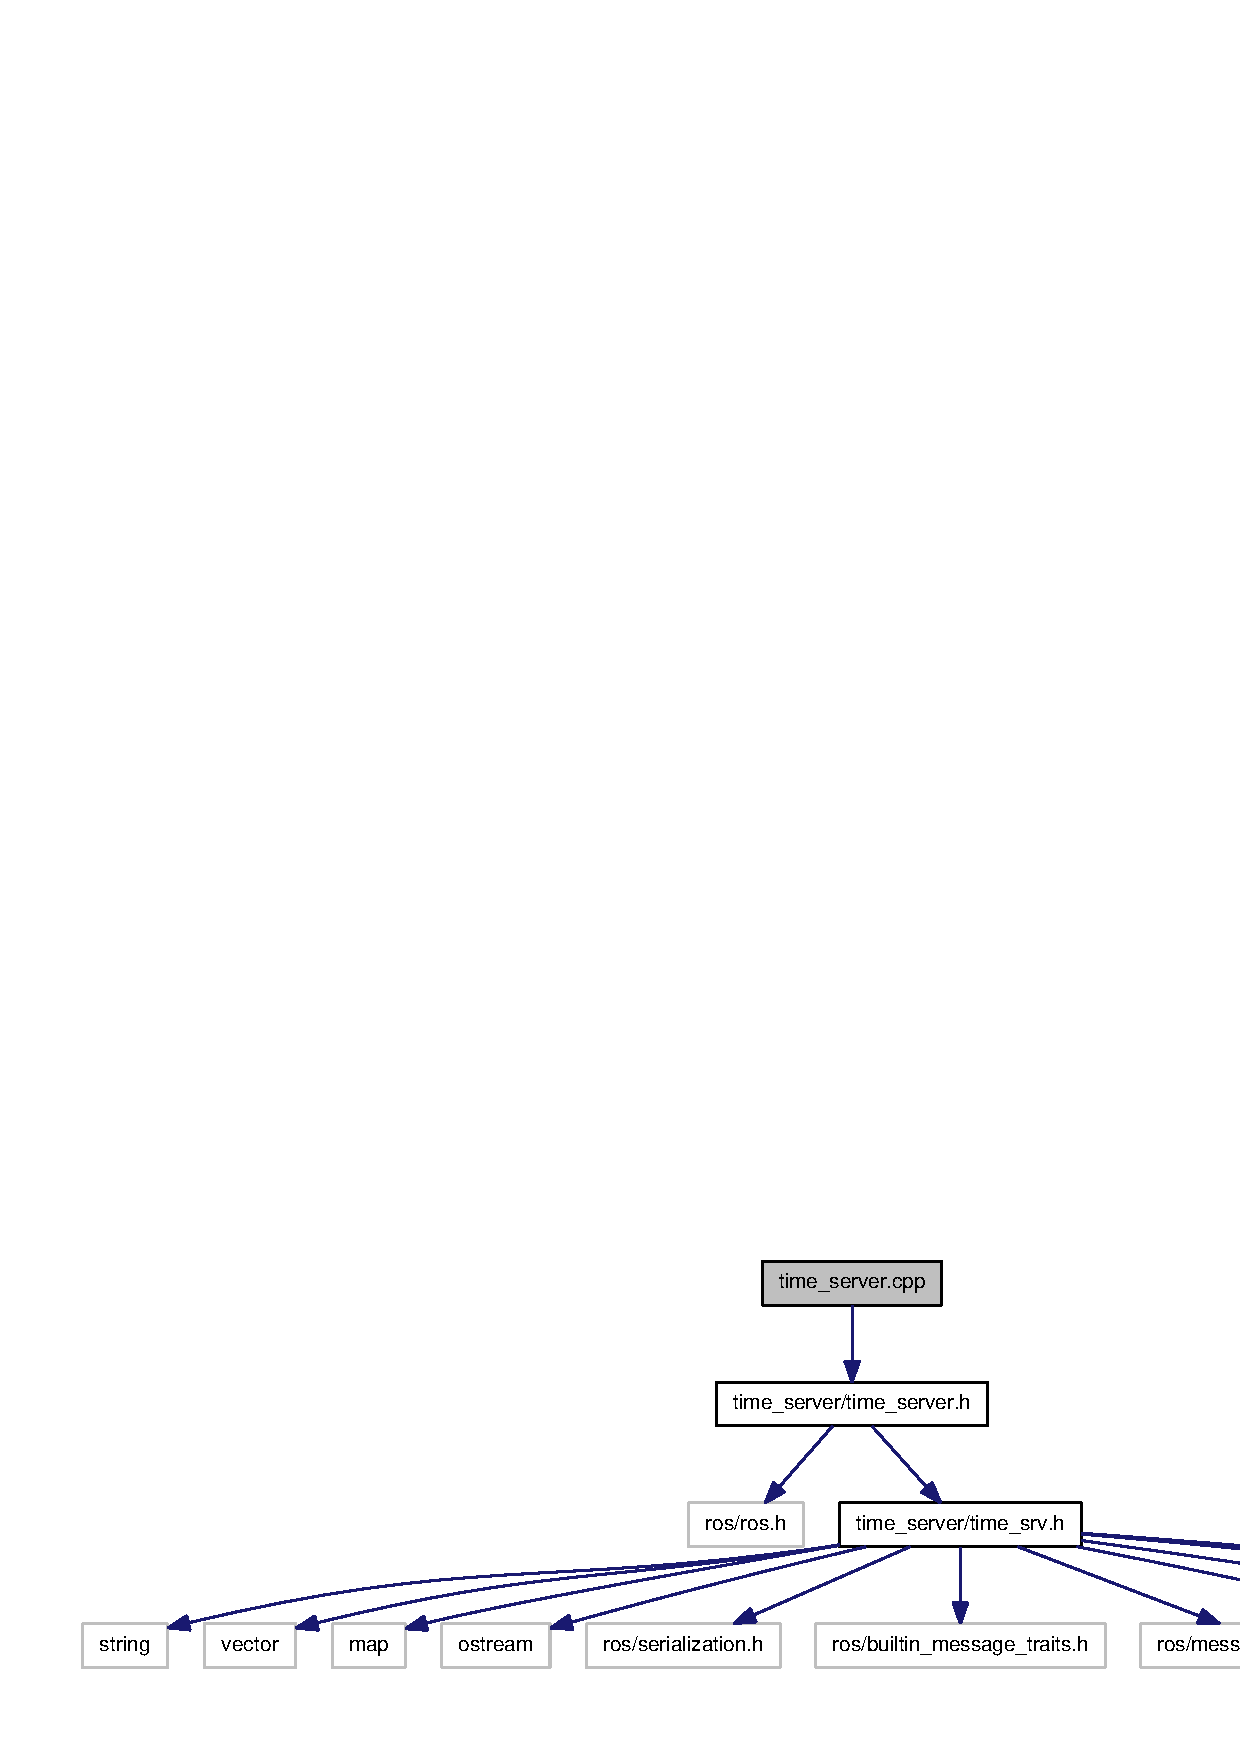
\includegraphics[width=350pt]{time__server_8cpp__incl}
\end{center}
\end{figure}
\subsection*{\-Functions}
\begin{DoxyCompactItemize}
\item 
int {\bf main} (int argc, char $\ast$$\ast$argv)
\begin{DoxyCompactList}\small\item\em \-Creates an instance of the node. \end{DoxyCompactList}\end{DoxyCompactItemize}


\subsection{\-Function \-Documentation}
\index{time\-\_\-server.\-cpp@{time\-\_\-server.\-cpp}!main@{main}}
\index{main@{main}!time_server.cpp@{time\-\_\-server.\-cpp}}
\subsubsection[{main}]{\setlength{\rightskip}{0pt plus 5cm}int {\bf main} (
\begin{DoxyParamCaption}
\item[{int}]{argc, }
\item[{char $\ast$$\ast$}]{argv}
\end{DoxyParamCaption}
)}\label{time__server_8cpp_a3c04138a5bfe5d72780bb7e82a18e627}


\-Creates an instance of the node. 



\-Definition at line 60 of file time\-\_\-server.\-cpp.


\section{time\-\_\-server.\-h \-File \-Reference}
\label{time__server_8h}\index{time\-\_\-server.\-h@{time\-\_\-server.\-h}}
{\ttfamily \#include \char`\"{}ros/ros.\-h\char`\"{}}\*
{\ttfamily \#include \char`\"{}time\-\_\-server/time\-\_\-srv.\-h\char`\"{}}\*
\-Include dependency graph for time\-\_\-server.\-h\-:\nopagebreak
\begin{figure}[H]
\begin{center}
\leavevmode
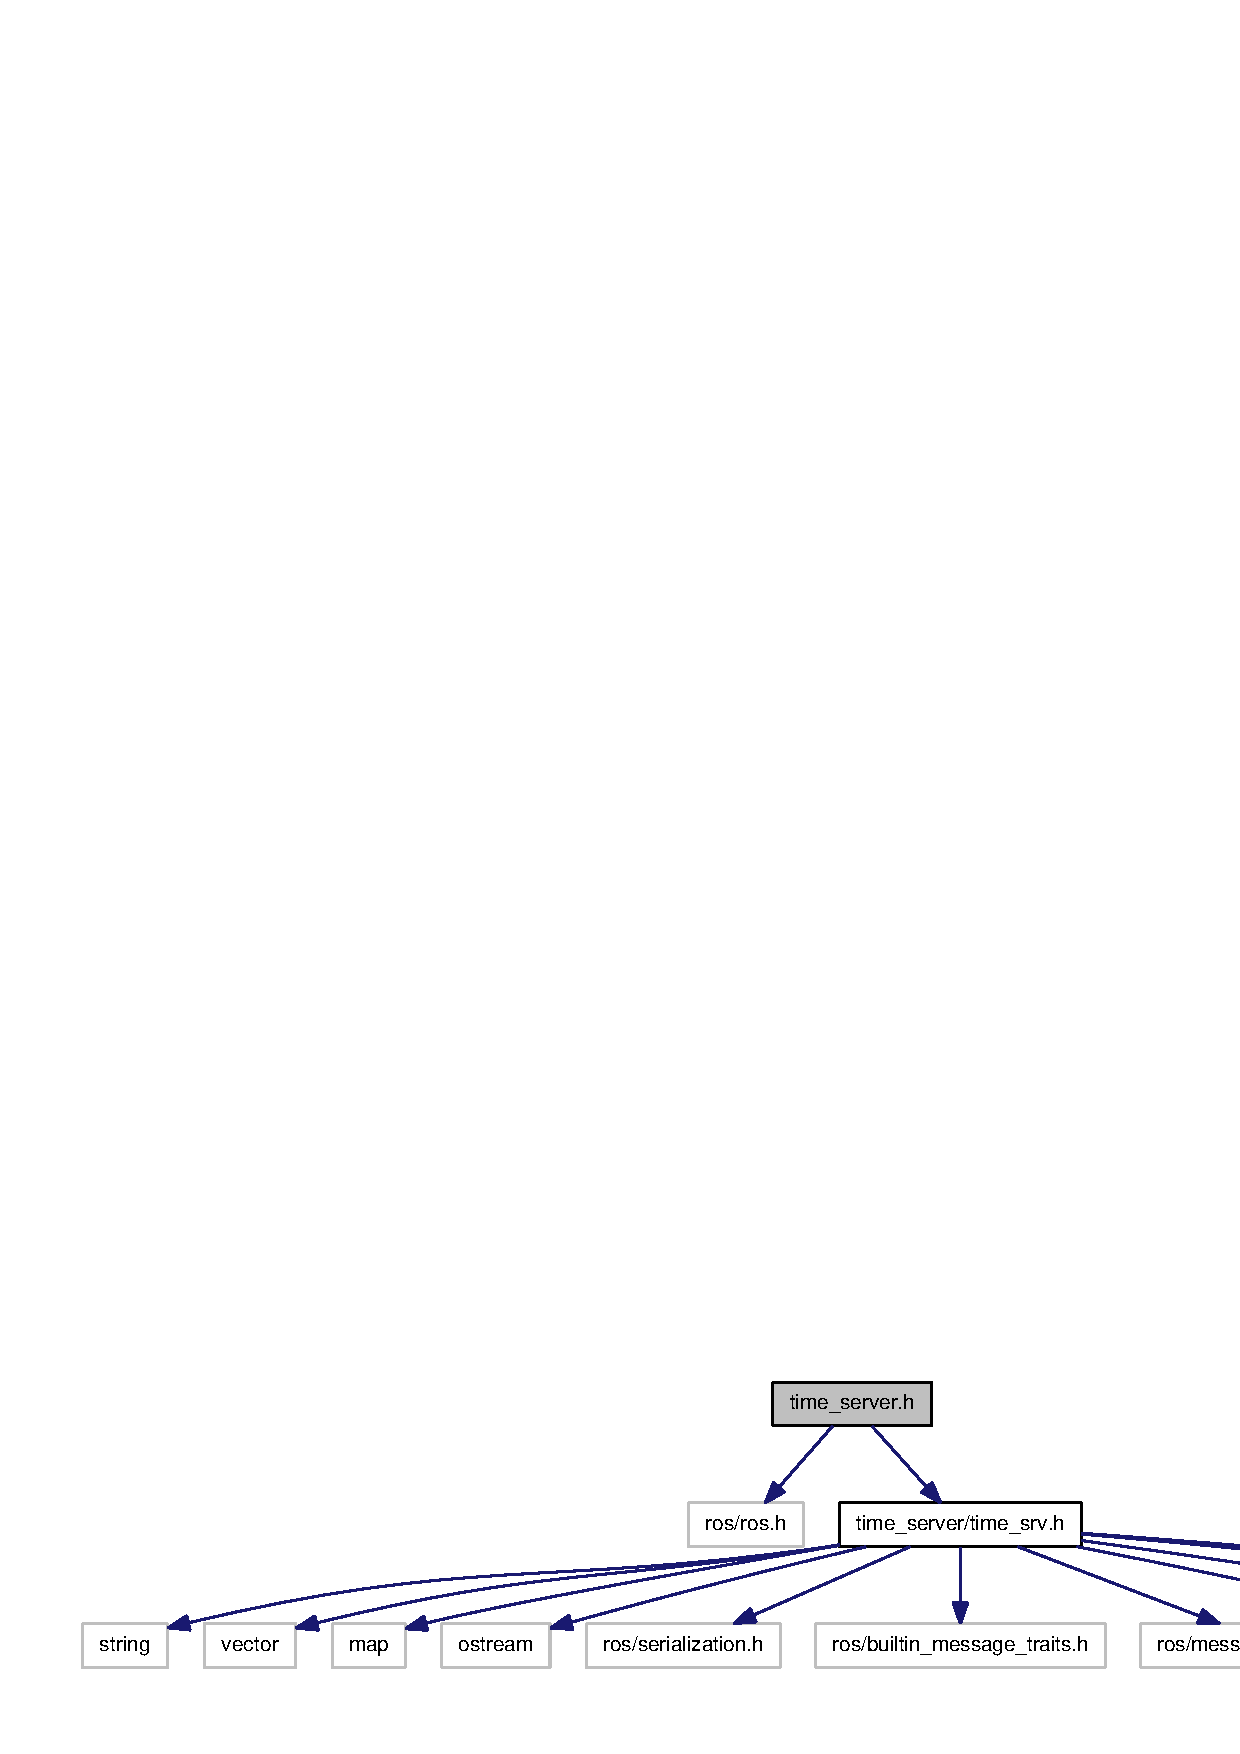
\includegraphics[width=350pt]{time__server_8h__incl}
\end{center}
\end{figure}
\-This graph shows which files directly or indirectly include this file\-:\nopagebreak
\begin{figure}[H]
\begin{center}
\leavevmode
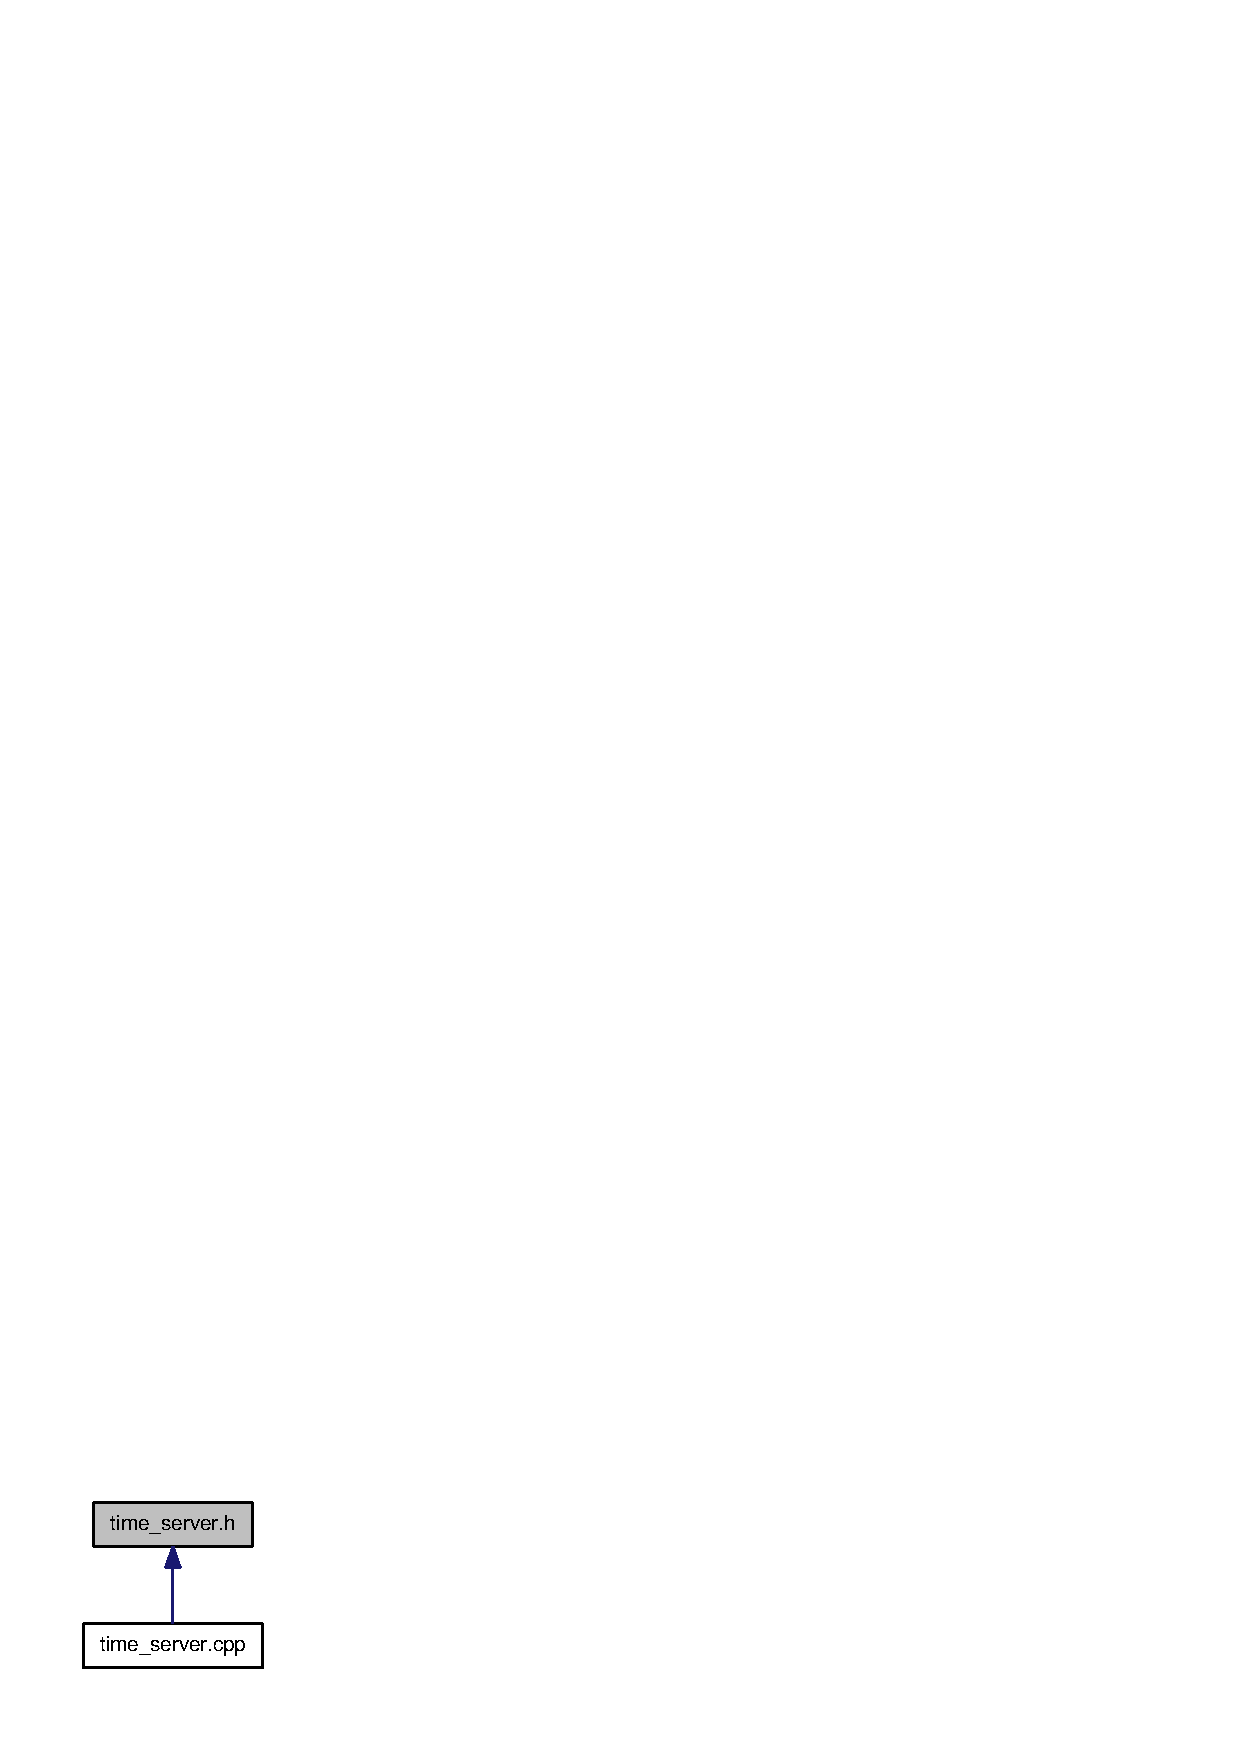
\includegraphics[width=130pt]{time__server_8h__dep__incl}
\end{center}
\end{figure}
\subsection*{\-Classes}
\begin{DoxyCompactItemize}
\item 
class {\bf \-Time\-Server}
\begin{DoxyCompactList}\small\item\em \-Node that provides a time service to keep other nodes in sync. \end{DoxyCompactList}\end{DoxyCompactItemize}

\section{time\-\_\-srv.\-h \-File \-Reference}
\label{time__srv_8h}\index{time\-\_\-srv.\-h@{time\-\_\-srv.\-h}}
{\ttfamily \#include $<$string$>$}\*
{\ttfamily \#include $<$vector$>$}\*
{\ttfamily \#include $<$map$>$}\*
{\ttfamily \#include $<$ostream$>$}\*
{\ttfamily \#include \char`\"{}ros/serialization.\-h\char`\"{}}\*
{\ttfamily \#include \char`\"{}ros/builtin\-\_\-message\-\_\-traits.\-h\char`\"{}}\*
{\ttfamily \#include \char`\"{}ros/message\-\_\-operations.\-h\char`\"{}}\*
{\ttfamily \#include \char`\"{}ros/time.\-h\char`\"{}}\*
{\ttfamily \#include \char`\"{}ros/macros.\-h\char`\"{}}\*
{\ttfamily \#include \char`\"{}ros/assert.\-h\char`\"{}}\*
{\ttfamily \#include \char`\"{}ros/service\-\_\-traits.\-h\char`\"{}}\*
\-Include dependency graph for time\-\_\-srv.\-h\-:\nopagebreak
\begin{figure}[H]
\begin{center}
\leavevmode
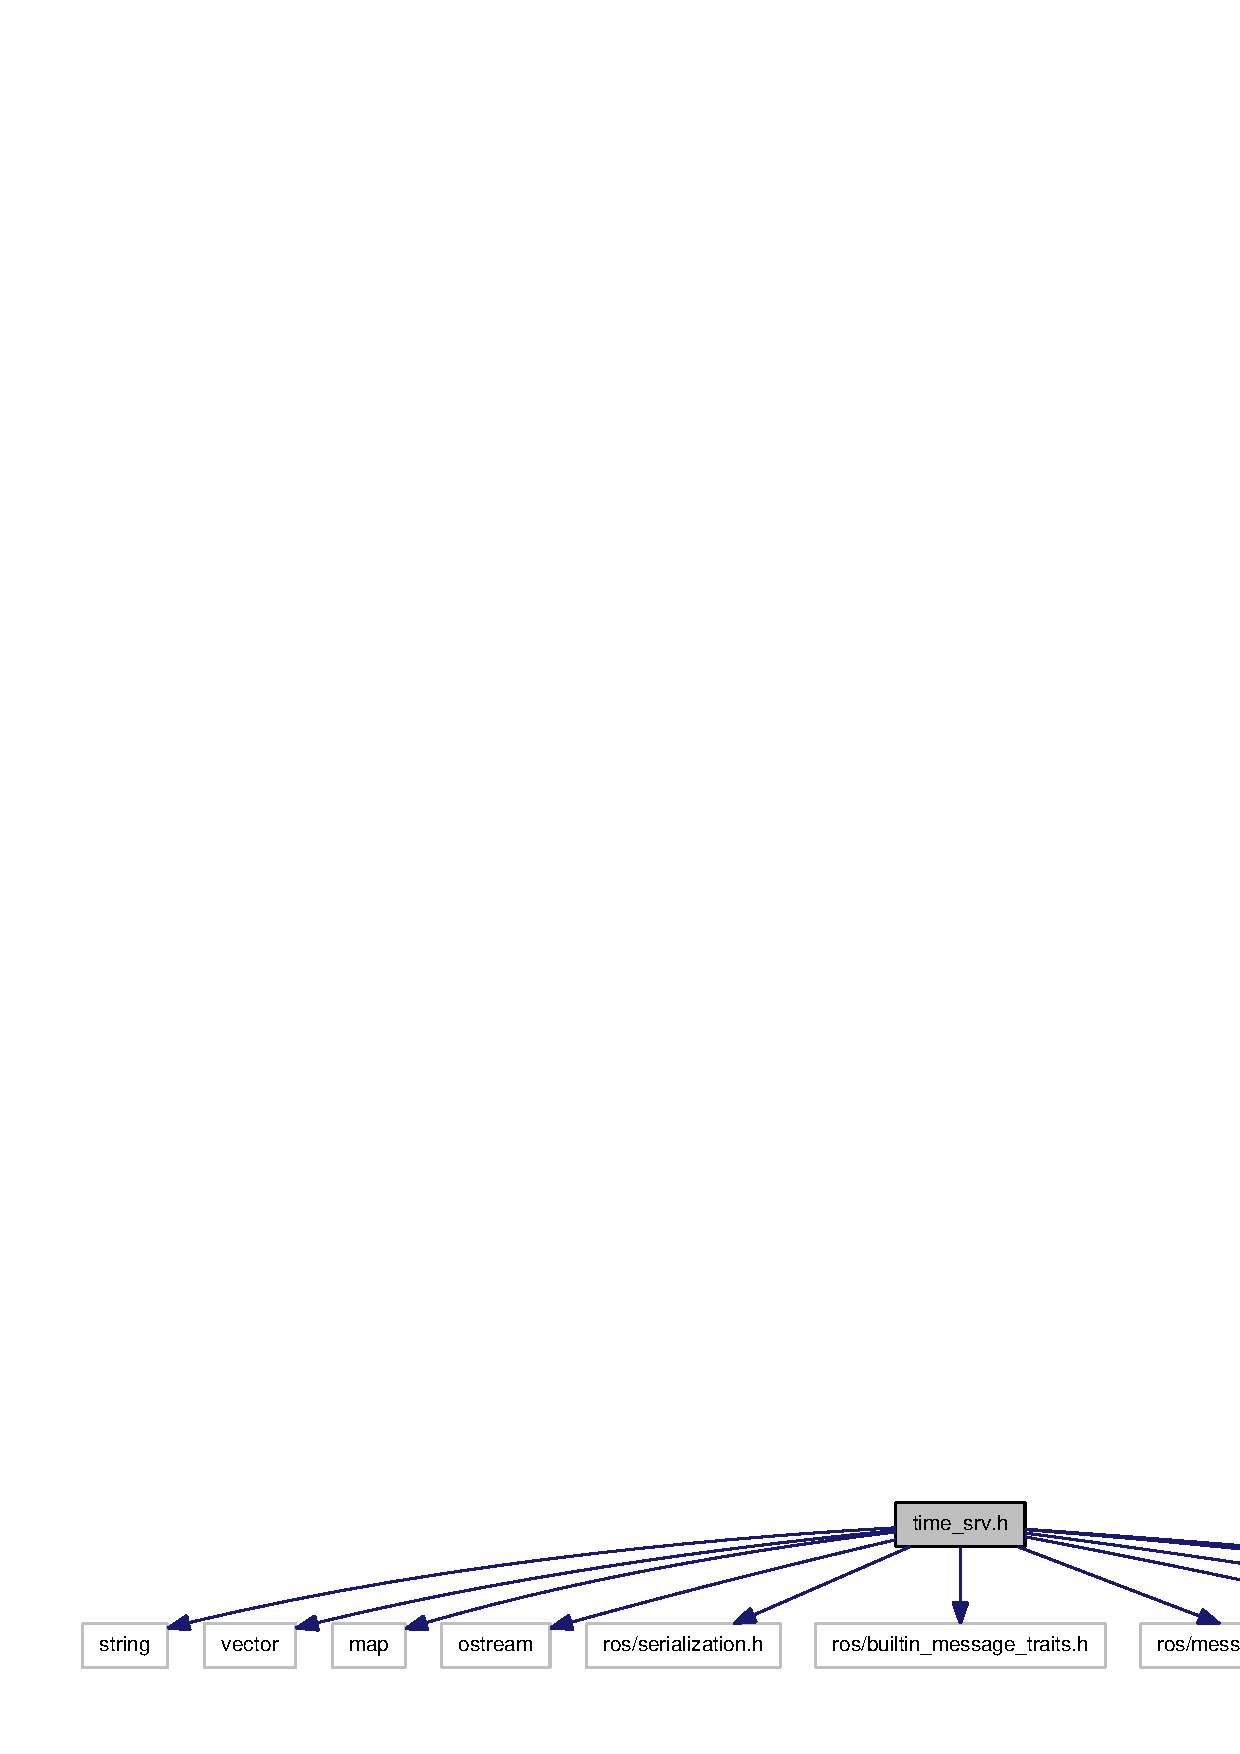
\includegraphics[width=350pt]{time__srv_8h__incl}
\end{center}
\end{figure}
\-This graph shows which files directly or indirectly include this file\-:\nopagebreak
\begin{figure}[H]
\begin{center}
\leavevmode
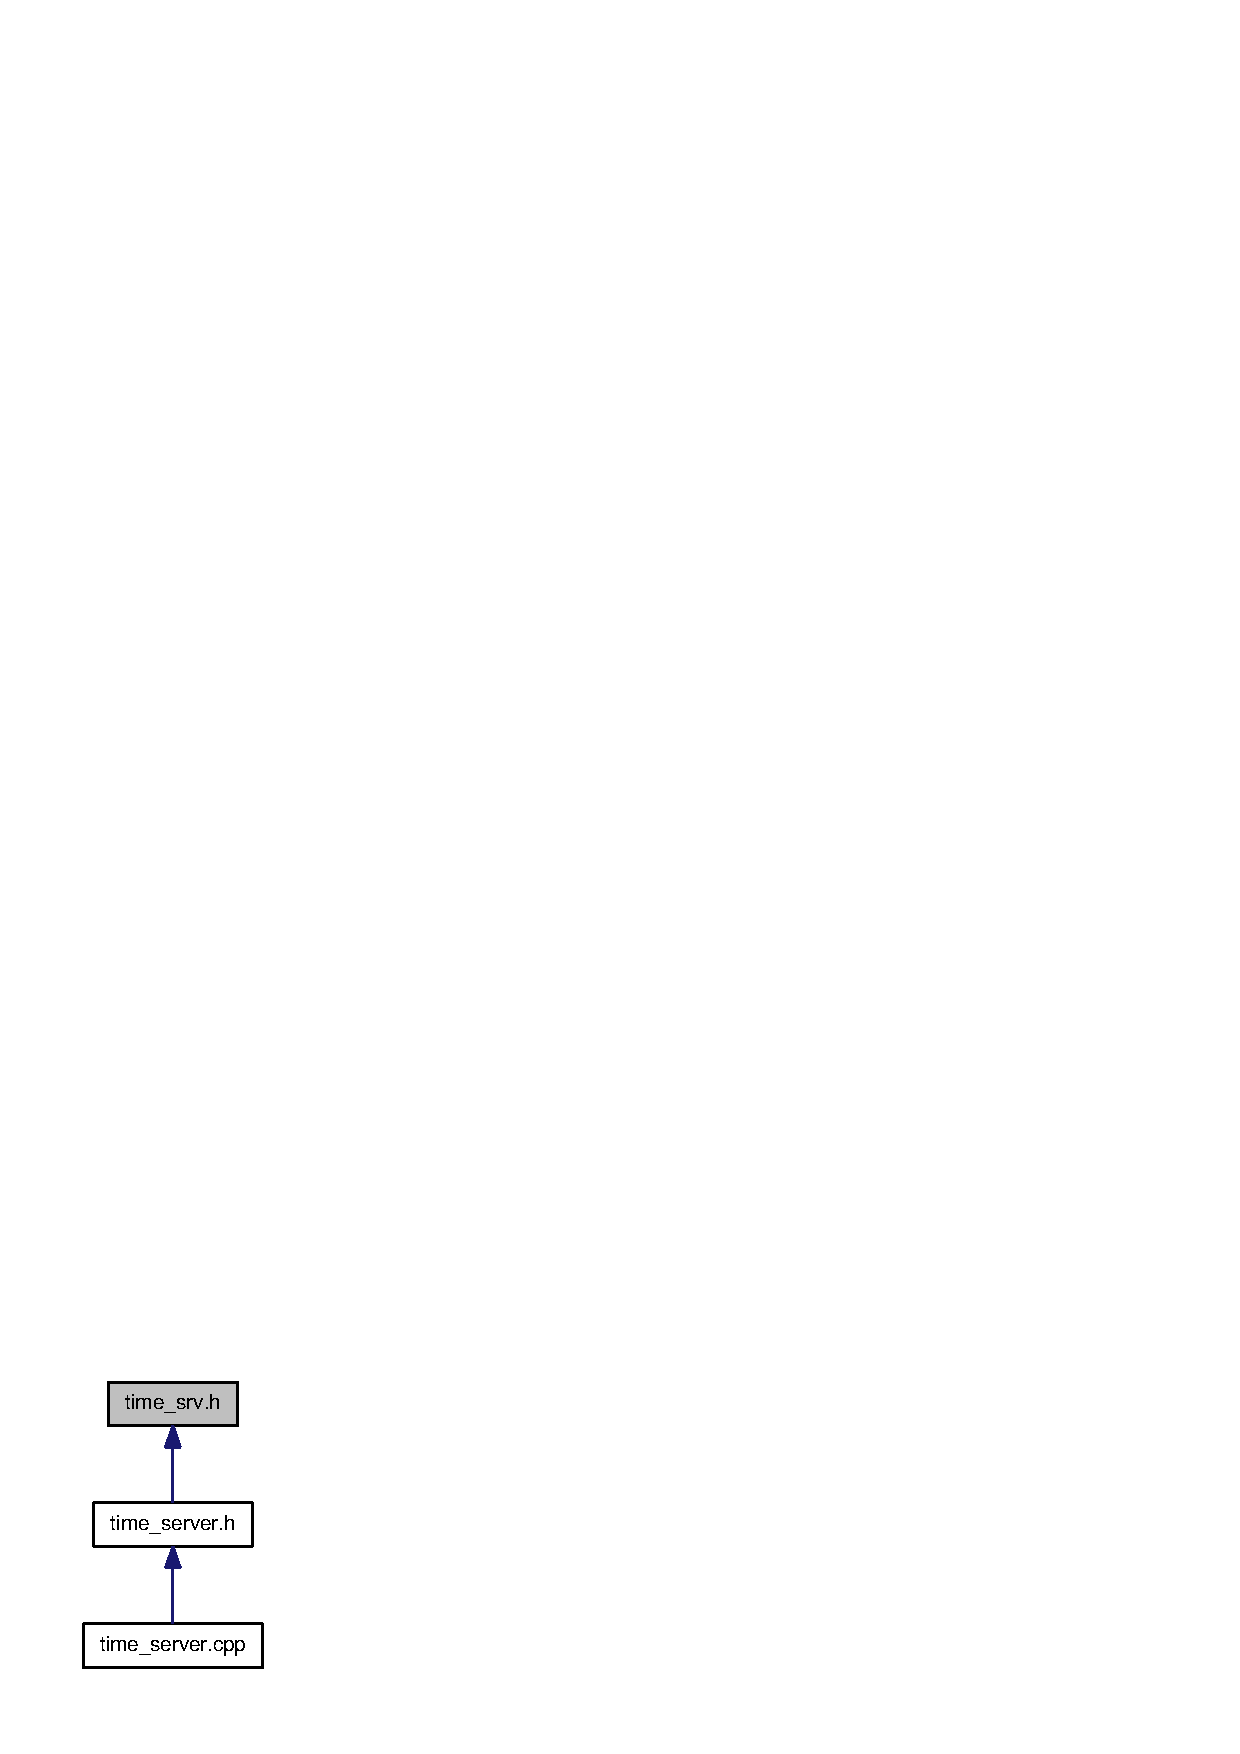
\includegraphics[width=130pt]{time__srv_8h__dep__incl}
\end{center}
\end{figure}
\subsection*{\-Classes}
\begin{DoxyCompactItemize}
\item 
struct {\bf ros\-::message\-\_\-traits\-::\-Data\-Type$<$ \-::time\-\_\-server\-::time\-\_\-srv\-Request\-\_\-$<$ Container\-Allocator $>$ $>$}
\item 
struct {\bf ros\-::message\-\_\-traits\-::\-Data\-Type$<$ \-::time\-\_\-server\-::time\-\_\-srv\-Response\-\_\-$<$ Container\-Allocator $>$ $>$}
\item 
struct {\bf ros\-::service\-\_\-traits\-::\-Data\-Type$<$ time\-\_\-server\-::time\-\_\-srv $>$}
\item 
struct {\bf ros\-::service\-\_\-traits\-::\-Data\-Type$<$ time\-\_\-server\-::time\-\_\-srv\-Request\-\_\-$<$ Container\-Allocator $>$ $>$}
\item 
struct {\bf ros\-::service\-\_\-traits\-::\-Data\-Type$<$ time\-\_\-server\-::time\-\_\-srv\-Response\-\_\-$<$ Container\-Allocator $>$ $>$}
\item 
struct {\bf ros\-::message\-\_\-traits\-::\-Definition$<$ \-::time\-\_\-server\-::time\-\_\-srv\-Request\-\_\-$<$ Container\-Allocator $>$ $>$}
\item 
struct {\bf ros\-::message\-\_\-traits\-::\-Definition$<$ \-::time\-\_\-server\-::time\-\_\-srv\-Response\-\_\-$<$ Container\-Allocator $>$ $>$}
\item 
struct {\bf ros\-::message\-\_\-traits\-::\-Is\-Fixed\-Size$<$ \-::time\-\_\-server\-::time\-\_\-srv\-Request\-\_\-$<$ Container\-Allocator $>$ $>$}
\item 
struct {\bf ros\-::message\-\_\-traits\-::\-Is\-Fixed\-Size$<$ \-::time\-\_\-server\-::time\-\_\-srv\-Response\-\_\-$<$ Container\-Allocator $>$ $>$}
\item 
struct {\bf ros\-::message\-\_\-traits\-::\-Is\-Message$<$ \-::time\-\_\-server\-::time\-\_\-srv\-Request\-\_\-$<$ Container\-Allocator $>$ $>$}
\item 
struct {\bf ros\-::message\-\_\-traits\-::\-Is\-Message$<$ \-::time\-\_\-server\-::time\-\_\-srv\-Request\-\_\-$<$ Container\-Allocator $>$const  $>$}
\item 
struct {\bf ros\-::message\-\_\-traits\-::\-Is\-Message$<$ \-::time\-\_\-server\-::time\-\_\-srv\-Response\-\_\-$<$ Container\-Allocator $>$ $>$}
\item 
struct {\bf ros\-::message\-\_\-traits\-::\-Is\-Message$<$ \-::time\-\_\-server\-::time\-\_\-srv\-Response\-\_\-$<$ Container\-Allocator $>$const  $>$}
\item 
struct {\bf ros\-::message\-\_\-traits\-::\-M\-D5\-Sum$<$ \-::time\-\_\-server\-::time\-\_\-srv\-Request\-\_\-$<$ Container\-Allocator $>$ $>$}
\item 
struct {\bf ros\-::message\-\_\-traits\-::\-M\-D5\-Sum$<$ \-::time\-\_\-server\-::time\-\_\-srv\-Response\-\_\-$<$ Container\-Allocator $>$ $>$}
\item 
struct {\bf ros\-::service\-\_\-traits\-::\-M\-D5\-Sum$<$ time\-\_\-server\-::time\-\_\-srv $>$}
\item 
struct {\bf ros\-::service\-\_\-traits\-::\-M\-D5\-Sum$<$ time\-\_\-server\-::time\-\_\-srv\-Request\-\_\-$<$ Container\-Allocator $>$ $>$}
\item 
struct {\bf ros\-::service\-\_\-traits\-::\-M\-D5\-Sum$<$ time\-\_\-server\-::time\-\_\-srv\-Response\-\_\-$<$ Container\-Allocator $>$ $>$}
\item 
struct {\bf ros\-::serialization\-::\-Serializer$<$ \-::time\-\_\-server\-::time\-\_\-srv\-Request\-\_\-$<$ Container\-Allocator $>$ $>$}
\item 
struct {\bf ros\-::serialization\-::\-Serializer$<$ \-::time\-\_\-server\-::time\-\_\-srv\-Response\-\_\-$<$ Container\-Allocator $>$ $>$}
\item 
struct {\bf time\-\_\-server\-::time\-\_\-srv}
\item 
struct {\bf time\-\_\-server\-::time\-\_\-srv\-Request\-\_\-$<$ Container\-Allocator $>$}
\item 
struct {\bf time\-\_\-server\-::time\-\_\-srv\-Response\-\_\-$<$ Container\-Allocator $>$}
\end{DoxyCompactItemize}
\subsection*{\-Namespaces}
\begin{DoxyCompactItemize}
\item 
namespace {\bf ros}
\item 
namespace {\bf ros\-::message\-\_\-traits}
\item 
namespace {\bf ros\-::serialization}
\item 
namespace {\bf ros\-::service\-\_\-traits}
\item 
namespace {\bf time\-\_\-server}
\end{DoxyCompactItemize}
\subsection*{\-Typedefs}
\begin{DoxyCompactItemize}
\item 
typedef \*
\-::{\bf time\-\_\-server\-::time\-\_\-srv\-Request\-\_\-}\*
$<$ std\-::allocator$<$ void $>$ $>$ {\bf time\-\_\-server\-::time\-\_\-srv\-Request}
\item 
typedef boost\-::shared\-\_\-ptr\*
$<$ \-::{\bf time\-\_\-server\-::time\-\_\-srv\-Request} \*
const  $>$ {\bf time\-\_\-server\-::time\-\_\-srv\-Request\-Const\-Ptr}
\item 
typedef boost\-::shared\-\_\-ptr\*
$<$ \-::{\bf time\-\_\-server\-::time\-\_\-srv\-Request} $>$ {\bf time\-\_\-server\-::time\-\_\-srv\-Request\-Ptr}
\item 
typedef \*
\-::{\bf time\-\_\-server\-::time\-\_\-srv\-Response\-\_\-}\*
$<$ std\-::allocator$<$ void $>$ $>$ {\bf time\-\_\-server\-::time\-\_\-srv\-Response}
\item 
typedef boost\-::shared\-\_\-ptr\*
$<$ \-::{\bf time\-\_\-server\-::time\-\_\-srv\-Response} \*
const  $>$ {\bf time\-\_\-server\-::time\-\_\-srv\-Response\-Const\-Ptr}
\item 
typedef boost\-::shared\-\_\-ptr\*
$<$ \-::{\bf time\-\_\-server\-::time\-\_\-srv\-Response} $>$ {\bf time\-\_\-server\-::time\-\_\-srv\-Response\-Ptr}
\end{DoxyCompactItemize}

\printindex
\end{document}
